% Template for B. Sc and M. Sc. (Tech.) degree programmes at the
% Faculty of Information Technology and Electrical Engineering
% at University of Oulu (CSE/BME/BA)
%
% Authors: Mika Korhonen (original author), Pekka Pietikäinen, Christian Wieser, Teemu Tokola, Juha Kylmänen, Tuomas Holmberg and Tuomas Varanka.
% If you make any improvements to this template, submit them via
% https://github.com/ouspg/cse-thesis
%
% Signing in to Overleaf with a oulu.fi account is strongly recommended, this gives students and staff
% access to a Professional subscription
%
% CHANGELOG
% 2023-01-31: Track changes has been turned on - TTo
% 2023-06-15: Improvements to avoid missing filling in some details: TODO's added to template (TTo)
% 2023-06-15: Changes to foreword, clarifications to indicate template is also for Bachelor thesis  (TTo)
% 2023-06-15: Example of a CC-BY figure added with reference in the footnotes (TTo)
% 2025-08-18: Major refactoring of the template (PPi)

%
% dithesis.cls supports the following options
% Language: english/finnish
% Degree programme: cse (default)/bme/ba
% Thesis type: master (default)/bachelor
% Output type: online (default, 2.5 cm margin)
%              print (4.5 cm left margin for bound theses)
\documentclass[english, online, cse, master]{dithesis}

%% Copyright of a work is with the creator/author of the work regardless of
%% whether the copyright mark is explicitly in the work or not. You may, if you
%% wish---we encourage you to do so---publish your work under a Creative
%% Commons license (see creativecommons.org), in which case the license text
%% must be visible in the work.

% Uncommenting one of the following will automatically create a copyright page
% If both are commented out the license is "All rights reserved"
% and no copyright page will be generated
%
%\IfLang{\MainLang}{finnish}{%
  \copyrighttext
  {\copyrightmetastring\ \allrightsreservedfin}%
  {%
    \copyrightstring\ \allrightsreservedfin
    \blockpar
    Työn yksityiskäyttö on sallittua. Kuvien uudelleenjulkaisu ja
    muokkaaminen ilman lupaa on kielletty.
  }
}
{%
  \copyrighttext%
  {\copyrightmetastring\ \allrightsreservedeng}%
  {%
    \copyrightstring\ \allrightsreservedeng
    \blockpar
    Private use of this thesis is permitted. Reproduction or
    modification of the figures without permission is prohibited.
  }
}

% Only include if you want to use a Creative Commons license,
% since otherwise undesired information may be included in the PDF metadata.
\usepackage[type={CC}, modifier={by}, version={4.0}]{doclicense-di}

\IfLang{\MainLang}{finnish}{%
  \copyrighttext
  {\copyrightmetastring\ Jos ei toisin mainita, tämän dokumentin käyttö
    on sallittu Creative Commons 4.0 Kansainvälinen (CC-BY-4.0)
  lisenssin mukaisesti.}
  {%
    \copyrightstring
    \doclicenseThis
  }
}
{%
  \copyrighttext%
  {\copyrightmetastring\ Except otherwise noted, the reuse of this
    document is authorized under a Creative Commons 4.0 International
  (CC-BY-4.0) license.}%
  {%
    \copyrightstring
    \doclicenseThis
  }
}


% TikZ for the architecture diagram in Chapter 3.
\usepackage{tikz}
\usetikzlibrary{arrows.meta, positioning, shapes.geometric}

% tcolorbox for the per-hypothesis verdict blocks in Chapter 4.
\usepackage[most]{tcolorbox}

% Absorb a few sub-line overfull boxes gracefully without hand-tuning
% individual lines (typographic polish; no effect on content).
\setlength{\emergencystretch}{1.5em}

% array: enables >{\raggedright\arraybackslash}p{} columns so fixed-width
% table cells break without justification-induced overfull boxes.
\usepackage{array}

%%%%%%%%%%%%%%%%%%%%% SET YOUR INFORMATION HERE %%%%%%%%%%%%%%%%%%%%%%%
%%%%%%%%%%%%%%%%%%%%%%%%%%%%%%%%%%%%%%%%%%%%%%%%%%%%%%%%%%%%%%%%%%%%%%%%%
% Both English and Finnish title are needed
\title{The Coordination Cliff: How Context Compression Breaks Multi-Fragment LLM Workflows}
\otsikko{Koordinaation jyrk\"anne: kuinka kontekstin tiivist\"aminen rikkoo monifragmenttisia kielimallity\"onkulkuja}

\firstname{Syed Abdullah}
\lastname{Hassan}

% Names of other authors can be added here
%\firstnametwo{}
%\lastnametwo{}
%\firstnamethree{}
%\lastnamethree{}
% Remove or comment the extra names if you do not need them

% Abstracts are stored in the PDF metadata.
% They must not contain empty lines (multiple paragraphs) or special
% characters. Mathematical symbols should work (mathxmp option of the pdfx
% package).
% If the abstract contains multiple paragraphs or special characters,
% provide the full text in abstract.tex and tiivistelma.tex.
% This version should otherwise remain identical to it
\abstract{Every token a multi-step LLM workflow reads costs energy,
  latency, and money, so context compression is the obvious lever.
  The prompt-compression literature is mature, but it is measured on
  single-fragment question-answering, whereas production workflows
  must combine information across several independently compressed
  fragments, and whether preserving single-fragment quality also
  preserves that harder property had never been tested. It does not:
  on a new 150-instance benchmark spanning cross-document fact
  aggregation, constraint-satisfaction planning, and multi-step
  retrieval, four training-free compressors swept over ten ratios show
  no positive workload-level correlation between source-retention F1
  (token overlap between each compressed fragment and its source) and
  multi-fragment coordination success (Spearman in [-0.82, +0.32], all
  95 percent bootstrap intervals excluding 0.6), so the single-agent
  benchmarks that dominate the field mis-rank compressors for
  multi-fragment deployment. The breakdown is abrupt: a sharp
  coordination cliff, present on 11 of 12 (compressor, family) cells,
  at which success collapses once compression strips the task-critical
  tokens a planner must combine; a compounding-error model explains
  the sharp transition and recovers its position to first order. The
  cliff is a property of the compressor and the task, not the planner:
  within a calibrated regime it shows no detected shift from a local
  Llama-3.1-8B to a frontier Qwen-2.5-72B across a 9x scale-up and a
  change of architecture family, and only extended-reasoning planners
  fall outside this regime. Beyond this negative result, the thesis
  delivers the benchmark, the coordination-cliff characterisation and
  its predictive model, evidence that compression also lowers
  protected-fact disclosure in proportion to how much text it destroys
  rather than through privacy-specific filtering, and a reproducible,
  policy-enforcing memory-bus reference implementation.}

\tiivistelma{Suuria kielimalleja k\"aytt\"av\"at monivaiheiset
  ty\"onkulut maksavat jokaisesta lukemastaan tokenista, ja
  kontekstin tiivist\"aminen on luonteva s\"a\"at\"okeino. Yhden
  agentin kehotteentiivist\"amist\"a koskeva kirjallisuus ei
  kuitenkaan mittaa sit\"a, s\"ailytt\"a\"ak\"o
  kysymys-vastaus-tarkkuutta s\"ailytt\"av\"a tiivist\"aminen
  my\"os sit\"a vaikeampaa ominaisuutta, jonka suunnittelija
  tarvitsee: useaan tiivistettyyn fragmenttiin jaetun tiedon
  yhdist\"amist\"a oikeaksi vastaukseksi. T\"am\"a tutkielma
  tarkastelee kysymyst\"a monifragmenttisilla
  kielimallity\"onkuluilla. Arvioinnissa suunnittelijana toimii
  joko deterministinen regex-j\"asennin tai yksi kielimallikutsu,
  jossa kaikki tiivistetyt fragmentit ovat n\"akyvill\"a;
  monikierroksinen agenttisimulointi on rajattu empiirisen
  tarkastelun ulkopuolelle. Ty\"o esitt\"a\"a nelj\"a p\"a\"atulosta.
  Toistettava koordinaation vertailutesti, jossa on 150 instanssia
  kolmesta ty\"okuormaperheest\"a. Empiirinen kuvaus koordinaation
  jyrk\"anteest\"a yhdess\"a kumuloituvan virheen mallin kanssa,
  joka selitt\"a\"a jyrk\"anteen kynnysrakenteen ja palauttaa
  empiirisen sijainnin ensimm\"aisen kertaluvun tarkkuudella
  kierroskohtaisesta token-recallista. Havainto, jonka mukaan
  kalibroidulla alueella jyrk\"anteen sijainnissa ei havaita
  siirtym\"a\"a paikallisen Llama-3.1-8B-suunnittelijan ja
  huipputason Qwen-2.5-72B-suunnittelijan v\"alill\"a, DeepSeek V4
  Pro:n vahvistaessa tuloksen heikosti. Sek\"a kolmen RAG-putken
  katalogi, jossa tiivist\"a-ensin-j\"arjestys osoittautuu yhdess\"a
  testatussa upotus- ja indeksipinossa johdonmukaisesti mutta vain
  kohtuullisesti paremmaksi (2--3 prosenttiyksik\"on F1-ero) kuin
  hae-ensin-j\"arjestys. Lis\"aksi ty\"o toimittaa muistiv\"ayl\"an
  viitetoteutuksen ja yhteenvetotason p\"a\"attelyilmaisumetriikan.
  P\"a\"atulokset: yhden fragmentin tiedon s\"ailyminen ei ennusta
  positiivisesti koordinaation onnistumista mill\"a\"an testatulla
  tiivist\"aj\"all\"a; jyrkk\"a jyrk\"anne on olemassa; suunnittelijan
  kapasiteetti m\"a\"aritt\"a\"a onnistumiskaton mutta ei
  jyrk\"anteen sijaintia kalibroidulla alueella; informaation tiheys
  skaalaa jyrk\"annett\"a aineistojen v\"alill\"a; ja tiivist\"aminen
  v\"ahent\"a\"a mitattavasti suojattujen faktojen
  p\"a\"attelyilmaisua. Jyrk\"annetietoinen adaptiivinen k\"a\"are
  CAAC operationaalistaa kumuloituvan virheen rajan ajonaikaisena
  per\"a\"antymismekanismina.}


% Keywords are also included in the PDF metadata, and cannot contain any
% special characters. Separate them with \spc
\keywords{context compression\spc large language models\spc coordination cliff\spc multi-fragment workflows\spc memory bus\spc inference disclosure\spc agentic memory\spc retrieval-augmented generation}
\avainsanat{kontekstin tiivist\"aminen\spc suuret kielimallit\spc koordinaatiojyrk\"anne\spc monifragmenttiset ty\"onkulut\spc muistiv\"ayl\"a\spc p\"a\"attelyilmaisu\spc agenttinen muisti\spc hakuparannettu generointi}


%%%%%%%%%%%%%%%%%%%%%%%%%%%%%%%%%%%%%%%%%%%%%%%%%%%%%%%%%%%%%%%%%%%%%%%%%
%%%%%%%%%%%%%%%%%%%%%%%%%%%%%%%%%%%%%%%%%%%%%%%%%%%%%%%%%%%%%%%%%%%%%%%%%
% \headertitlecap automatically creates headers with TitleCaps
% (Capitalizes the First Letter in Each Word except ``Small'' Ones)
% https://en.wikipedia.org/wiki/Title_case
% This only has effect in English. In Finnish headers follow
% the normal Finnish rules of capitalization.
%
% Title (abstract page, on front page it is all caps)
% Chapters are all caps
% Sections are title case
% Subsections are title case
% Subsubsections are in sentence case (as in IEEE Style manual)
% Words not to be capitalized can be changed in dithesis.sty.
%
% Note that this does not affect the PDF table of contents, which is stored
% in the metadata.
% Because of this, you should consistently capitalize headers in your .tex
% Both normal (sentence) case and title case are acceptable.
% This template uses sentence case.
\headertitlecap

% Add your bibliographies here. You can use several with BibLaTeX.
\addbibresource{citations.bib}

\begin{document}
\pagestyle{empty}
\maketitlepage
\makecopyrightpage

\IfLang{\MainLang}{finnish}{
  \begin{thesisabstract}{finnish}

Suuria kielimalleja hyödyntävät monivaiheiset työnkulut
maksavat jokaisesta lukemastaan tokenista, joten
kontekstin tiivistäminen on luonteva keino karsia
kustannuksia. Tiivistämistä mitataan kuitenkin yhden
fragmentin kysymys--vastaus-tarkkuudella, vaikka
tuotannon työkuormat yhdistävät tietoa useasta erikseen
tiivistetystä fragmentista. Sitä, säilyttääkö yhden
fragmentin laadun säilyttävä tiivistäminen myös tämän
vaikeamman ominaisuuden, ei ollut aiemmin tutkittu.

Ei säilytä. Uudessa $150$ instanssin vertailuaineistossa
neljä ilman koulutusta toimivaa tiivistäjää kymmenen
tiivistyssuhteen yli ei tuota lainkaan positiivista
työkuormatason korrelaatiota lähdesäilyvyys-F1:n ja
koordinaation onnistumisen välille (Spearmanin
järjestyskorrelaatio $[-0{,}82, +0{,}32]$). Romahdus on
äkillinen: jyrkkä koordinaation jyrkänne $\tau^{*}$
esiintyy $11$ solussa $12$:sta, kun tiivistäminen karsii
ne kriittiset tokenit, jotka suunnittelijan on
yhdistettävä. Kumuloituvan virheen malli selittää
kynnyksen ja palauttaa sen sijainnin ensimmäisen
kertaluvun tarkkuudella. Jyrkänne on tiivistäjän ja
tehtävän, ei suunnittelijan, ominaisuus: kalibroidulla
alueella sen sijainti ei siirry paikallisesta
Llama-3.1-8B:stä huipputason Qwen-2.5-72B:hen.

Työn tuloksena on käytäntöjä valvova muistiväylä, joka
tiivistää jokaisen fragmentin matkalla ja muuntaa
tokensäästöt suoraan pienemmäksi päättelykustannukseksi.
Sen tiivistystä ohjaa mittauksiin perustuva
jyrkännetietoinen kääre (CAAC), joka perääntyy
aggressiivisimpaan suhteeseen, joka pitää kunkin
fragmentin jyrkänteen turvalliselle puolelle. Avoimen
lähdekoodin viitetoteutus on toistettavissa yhdellä
komennolla esilasketun tiivistysvälimuistin avulla.

\end{thesisabstract}

  \begin{thesisabstract}{english}

Large language models running in multi-step workflows pay for every
token they read: energy, latency, and cost scale with context
length, and much of that context carries little information. Context
compression is the natural lever, and the single-agent
prompt-compression literature is mature. What has not been measured
is whether a compressor that preserves single-agent
question-answering accuracy also preserves the harder property a
planner needs --- combining information distributed across several
compressed fragments into a correct answer. This thesis measures
that on \emph{multi-fragment LLM workflows}, using a deterministic
regex solver or a single LLM call over all compressed fragments as
the planner; multi-round agent simulation is outside the empirical
scope.

The headline contribution is the H1 finding above. Three further
contributions support it. \textbf{C1} is a reproducible
$150$-instance multi-fragment benchmark across three workload
families (cross-document fact aggregation, constraint-satisfaction
planning, multi-step retrieval). \textbf{C2} is the empirical
characterisation itself --- a sharp \emph{coordination cliff}
$\tau^{*}$ across four training-free compressors, together with a
compounding-error model whose contribution is explaining \emph{why}
the transition is sharp (a recall threshold on critical tokens
produces a step in success); position prediction is a
\emph{first-order} estimate only (median relative error $\approx
35\%$, predicted band misses the empirical $\tau^{*}$ on $11/11$
testable cells). A direct A3 probe with an LLM planner --- the only
non-circular test of the threshold mechanism --- confirms the step
shape on the dense family ($k\approx 15$, $r_0 \approx 0.84$) and a
graded transition on the distributed family ($k \approx 5.9$, band
$\approx 0.54$). \textbf{C3} is a three-pipeline RAG catalogue with
a first-pass EUR-per-workflow cost ledger whose corpus-dominated
fidelity limits the P3-vs-P1 comparison (no cost-parity claim is
made). \textbf{C4} is a memory-bus reference implementation
together with a summary-level \emph{inference-disclosure} metric;
the metric is the C4 \emph{research} contribution and the bus is
the engineering artefact that operationalises it. CAAC operationalises
the compounding-error bound as a runtime back-off and serves as a
constructive demonstration of the cliff measurement rather than a
fifth headline contribution.

The central result is \textbf{H1}: at the workload level ($n=150$),
the change in single-agent QA-F1 under compression does not
positively predict the change in coordination success for any of the
four compressors (Spearman $\rho \in [-0.82, +0.32]$; all
$95\%$~bootstrap CIs exclude $0.6$). The single-agent benchmarks
that dominate the compression literature therefore mis-rank
compressors for multi-fragment use. A sharp cliff exists on $11$ of
$12$ (compressor, family) cells. Within a defined calibrated regime
the \emph{LLM-planner} cliff shows no detected shift across a single
well-identified scale-and-architecture comparison (local
Llama-3.1-8B $\tau^{*}\approx 2.48$ vs frontier Qwen-2.5-72B
$\approx 2.79$ on one cell); a third frontier model (DeepSeek~V4~Pro)
corroborates only weakly with a bootstrap CI too wide to identify
the position. The RAG sign-flip hypothesis is not supported ---
compress-first is preferred over retrieve-first on the single
retriever/embedder stack tested --- and compression reduces
inference disclosure, but in proportion to how aggressively it
destroys source tokens rather than through privacy-specific
filtering (an oracle field-redaction control achieves the same
$\sim 23$~pp reduction at near-zero compression, matching the
truncation baseline at $-24.6$~pp). The H1 result on family-a should
be read with one structural caveat: that family's regex solver
succeeds iff enough critical numeric tokens survive compression, and
the critical-token-recall metric \emph{is} that surviving fraction,
so the model's central equation on family-a relates two near-identical
measurements --- it is most directly \emph{computable} on family-a,
not most independently \emph{validating}.

In the interest of honesty: of the six pre-registered hypotheses,
two hold as stated (H1, H2) and the rest were reframed or not
supported as originally written (the H3 sign-flip; the H5
monotonicity claim, reframed as ceiling--cliff separation; the H6
transfer claim, reframed as information-density scaling); the
compounding-error model is a first-order, not a tight, position
predictor. These reframings are reported explicitly. The deliverable
is the manuscript and an open-source reference implementation: the
local pipeline reproduces from one command given a precomputed
compression cache, while the frontier-API arm is reproducible in
distribution rather than byte-for-byte.

\end{thesisabstract}

  \selectlanguage{finnish}
} {
  \begin{thesisabstract}{english}

Large language models running in multi-step workflows pay for every
token they read: energy, latency, and cost scale with context
length, and much of that context carries little information. Context
compression is the natural lever, and the single-agent
prompt-compression literature is mature. What has not been measured
is whether a compressor that preserves single-agent
question-answering accuracy also preserves the harder property a
planner needs --- combining information distributed across several
compressed fragments into a correct answer. This thesis measures
that on \emph{multi-fragment LLM workflows}, using a deterministic
regex solver or a single LLM call over all compressed fragments as
the planner; multi-round agent simulation is outside the empirical
scope.

The headline contribution is the H1 finding above. Three further
contributions support it. \textbf{C1} is a reproducible
$150$-instance multi-fragment benchmark across three workload
families (cross-document fact aggregation, constraint-satisfaction
planning, multi-step retrieval). \textbf{C2} is the empirical
characterisation itself --- a sharp \emph{coordination cliff}
$\tau^{*}$ across four training-free compressors, together with a
compounding-error model whose contribution is explaining \emph{why}
the transition is sharp (a recall threshold on critical tokens
produces a step in success); position prediction is a
\emph{first-order} estimate only (median relative error $\approx
35\%$, predicted band misses the empirical $\tau^{*}$ on $11/11$
testable cells). A direct A3 probe with an LLM planner --- the only
non-circular test of the threshold mechanism --- confirms the step
shape on the dense family ($k\approx 15$, $r_0 \approx 0.84$) and a
graded transition on the distributed family ($k \approx 5.9$, band
$\approx 0.54$). \textbf{C3} is a three-pipeline RAG catalogue with
a first-pass EUR-per-workflow cost ledger whose corpus-dominated
fidelity limits the P3-vs-P1 comparison (no cost-parity claim is
made). \textbf{C4} is a memory-bus reference implementation
together with a summary-level \emph{inference-disclosure} metric;
the metric is the C4 \emph{research} contribution and the bus is
the engineering artefact that operationalises it. CAAC operationalises
the compounding-error bound as a runtime back-off and serves as a
constructive demonstration of the cliff measurement rather than a
fifth headline contribution.

The central result is \textbf{H1}: at the workload level ($n=150$),
the change in single-agent QA-F1 under compression does not
positively predict the change in coordination success for any of the
four compressors (Spearman $\rho \in [-0.82, +0.32]$; all
$95\%$~bootstrap CIs exclude $0.6$). The single-agent benchmarks
that dominate the compression literature therefore mis-rank
compressors for multi-fragment use. A sharp cliff exists on $11$ of
$12$ (compressor, family) cells. Within a defined calibrated regime
the \emph{LLM-planner} cliff shows no detected shift across a single
well-identified scale-and-architecture comparison (local
Llama-3.1-8B $\tau^{*}\approx 2.48$ vs frontier Qwen-2.5-72B
$\approx 2.79$ on one cell); a third frontier model (DeepSeek~V4~Pro)
corroborates only weakly with a bootstrap CI too wide to identify
the position. The RAG sign-flip hypothesis is not supported ---
compress-first is preferred over retrieve-first on the single
retriever/embedder stack tested --- and compression reduces
inference disclosure, but in proportion to how aggressively it
destroys source tokens rather than through privacy-specific
filtering (an oracle field-redaction control achieves the same
$\sim 23$~pp reduction at near-zero compression, matching the
truncation baseline at $-24.6$~pp). The H1 result on family-a should
be read with one structural caveat: that family's regex solver
succeeds iff enough critical numeric tokens survive compression, and
the critical-token-recall metric \emph{is} that surviving fraction,
so the model's central equation on family-a relates two near-identical
measurements --- it is most directly \emph{computable} on family-a,
not most independently \emph{validating}.

In the interest of honesty: of the six pre-registered hypotheses,
two hold as stated (H1, H2) and the rest were reframed or not
supported as originally written (the H3 sign-flip; the H5
monotonicity claim, reframed as ceiling--cliff separation; the H6
transfer claim, reframed as information-density scaling); the
compounding-error model is a first-order, not a tight, position
predictor. These reframings are reported explicitly. The deliverable
is the manuscript and an open-source reference implementation: the
local pipeline reproduces from one command given a precomputed
compression cache, while the frontier-API arm is reproducible in
distribution rather than byte-for-byte.

\end{thesisabstract}

  \begin{thesisabstract}{finnish}

Suuria kielimalleja hyödyntävät monivaiheiset työnkulut
maksavat jokaisesta lukemastaan tokenista, joten
kontekstin tiivistäminen on luonteva keino karsia
kustannuksia. Tiivistämistä mitataan kuitenkin yhden
fragmentin kysymys--vastaus-tarkkuudella, vaikka
tuotannon työkuormat yhdistävät tietoa useasta erikseen
tiivistetystä fragmentista. Sitä, säilyttääkö yhden
fragmentin laadun säilyttävä tiivistäminen myös tämän
vaikeamman ominaisuuden, ei ollut aiemmin tutkittu.

Ei säilytä. Uudessa $150$ instanssin vertailuaineistossa
neljä ilman koulutusta toimivaa tiivistäjää kymmenen
tiivistyssuhteen yli ei tuota lainkaan positiivista
työkuormatason korrelaatiota lähdesäilyvyys-F1:n ja
koordinaation onnistumisen välille (Spearmanin
järjestyskorrelaatio $[-0{,}82, +0{,}32]$). Romahdus on
äkillinen: jyrkkä koordinaation jyrkänne $\tau^{*}$
esiintyy $11$ solussa $12$:sta, kun tiivistäminen karsii
ne kriittiset tokenit, jotka suunnittelijan on
yhdistettävä. Kumuloituvan virheen malli selittää
kynnyksen ja palauttaa sen sijainnin ensimmäisen
kertaluvun tarkkuudella. Jyrkänne on tiivistäjän ja
tehtävän, ei suunnittelijan, ominaisuus: kalibroidulla
alueella sen sijainti ei siirry paikallisesta
Llama-3.1-8B:stä huipputason Qwen-2.5-72B:hen.

Työn tuloksena on käytäntöjä valvova muistiväylä, joka
tiivistää jokaisen fragmentin matkalla ja muuntaa
tokensäästöt suoraan pienemmäksi päättelykustannukseksi.
Sen tiivistystä ohjaa mittauksiin perustuva
jyrkännetietoinen kääre (CAAC), joka perääntyy
aggressiivisimpaan suhteeseen, joka pitää kunkin
fragmentin jyrkänteen turvalliselle puolelle. Avoimen
lähdekoodin viitetoteutus on toistettavissa yhdellä
komennolla esilasketun tiivistysvälimuistin avulla.

\end{thesisabstract}

  \selectlanguage{english}
}

\contents %Insert table of contents
\thispagestyle{empty}
\header{\headerforeword}

This thesis was carried out at the Future Computing Group, CSE Research Unit,
Faculty of Information Technology and Electrical Engineering, University of
Oulu, in collaboration with TalentAdore Ltd. The work was supervised
academically by Lauri Lov\'en, with industrial supervision from Asim Nadeem,
Oskari Valkama, and Saku Valkama at TalentAdore.

My deepest thanks go to Lauri, whose constant and unwavering support and
patience carried this work from a vague idea to a finished thesis. He gave me
the latitude to chase an unfamiliar empirical question (how coordination
under compression behaves at institutional scale) and the steady, patient
guidance to keep the scope tight whenever it threatened to sprawl; I could
not have asked for a better supervisor. I am just as grateful to Asim Nadeem,
Oskari Valkama, and Saku Valkama at TalentAdore for their support throughout
the thesis, and for sharing TalentAdore's production cost structure, which
anchored the cost-per-workflow arm of the evaluation in a real industrial
setting.

The thesis was prepared on a single Apple M4 Pro 48~GB workstation with an
RTX~5090 32~GB GPU host on the Tailscale mesh for the compression
precomputation and the model-scaling and frontier-API sweeps. The compute
envelope, the reproducibility package, and the reference implementation
accompanying the thesis are described in Appendix~\ref{appendix}, Section~D.

This work was supported by the Technology Industries of Finland Centennial
Foundation (Teknologiateollisuuden 100-vuotiss\"a\"ati\"o) under grant
number~6193.

\paragraph*{On the use of AI tools.}
I leaned on generative-AI tools throughout this thesis (mainly Anthropic's
Claude through the Claude Code command-line interface), and they were a
genuine productivity boost: kicking ideas around, writing and debugging the
experiment and analysis code, and tightening the prose. I used them as a fast
assistant rather than an authority: the hypotheses, the experimental results,
and their interpretation are my own, checked against the on-disk data, and I
take responsibility for everything in this thesis. Used this way, the tools
made the work faster and the writing cleaner without standing in for the
thinking.

\renewcommand{\cityname}{Helsinki, }
\signature

\vfill
\begin{center}
  \IfFileExists{Figures/teknologiateollisuus-saatio.png}{%
    
\includegraphics[width=0.40\textwidth]{Figures/teknologiateollisuus-saatio.png}%
  }{}%
\end{center}

\header{\headerabbreviations}
\setlongtables
% According to updated thesis guidelines, lowercase Greek letters used as quantities
% are italicized. Uppercase Greek letters are upright.
\begin{longtable}[l]{p{3cm}p{0.7\textwidth}}

    ACL & access control list \\
    ADR & architecture decision record \\
    API & application programming interface \\
    BCa & bias-corrected and accelerated (bootstrap CI) \\
    CI & confidence interval \\
    C1\,$\dots$\,C4 & contributions one through four of this thesis \\
    CSE & Computer Science and Engineering \\
    DAG & directed acyclic graph \\
    D7 & doctoral track 7 (Federated Knowledge Orchestration) \\
    EM & exact match (QA metric) \\
    FAISS & Facebook AI Similarity Search \\
    FCG & Future Computing Group \\
    fp16 & 16-bit floating-point \\
    GGUF & GPT-Generated Unified Format (llama.cpp model file format) \\
    H1\,$\dots$\,H8 & hypotheses one through eight \\
    HNSW & hierarchical navigable small world (vector index) \\
    HTTP & hypertext transfer protocol \\
    int4 & 4-bit integer quantisation \\
    ICAE & in-context autoencoder \\
    ITEE & Information Technology and Electrical Engineering \\
    KV cache & key--value cache (transformer attention) \\
    LCS & longest common subsequence \\
    LLM & large language model \\
    LoRA & low-rank adaptation \\
    LRU & least recently used \\
    M0\,$\dots$\,M5 & sibling thesis projects (Publication DB, Contract DB, Moodle/Patio, etc.) \\
    MLX & Apple's native ML framework for Apple Silicon \\
    MPS & Metal Performance Shaders (Apple PyTorch backend) \\
    NCE & noise-contrastive estimation \\
    NIST AI RMF & NIST AI Risk Management Framework \\
    OAuth & open authorisation protocol \\
    OTel & OpenTelemetry \\
    P1\,$\dots$\,P3 & retrieval--compression pipeline variants one through three \\
    PEFT & parameter-efficient fine-tuning \\
    PII & personally identifiable information \\
    QA & question answering \\
    RAG & retrieval-augmented generation \\
    SQL & structured query language \\
    SQLite & a lightweight, embedded SQL database \\
    SSE & server-sent events \\
    TTL & time-to-live \\
    UUID & universally unique identifier \\
    WAL & write-ahead log \\
    \\
    $L_{\textrm{recon}}$ & token-level reconstruction loss \\
    $L_{\textrm{NCE}}$ & InfoNCE contrastive loss \\
    $L_{\textrm{tag}}$ & per-slot tag-prediction loss (C4 only) \\
    $\lambda$ & loss-term weighting coefficient \\
    $M$ & number of memory slots in the soft-prompt compressor \\
    $\rho$ & Spearman's rank correlation coefficient \\
    $\tau^{*}$ & coordination cliff compression ratio \\
    $r$ & nominal compression ratio (input/output token count) \\
    $\delta$ & Cliff's delta (ordinal effect size) \\
    $d$ & Cohen's $d$ (continuous effect size) \\

\end{longtable}
\setcounter{table}{0}


% Enables page numbers and sets the dots for numbered chapters in
% table of contents
\mainmatter

\chapter{Introduction}
  \label{introduction}
  \section{Motivation: Every Token Has a Cost}
\label{sec:motivation}

Large language models pay for every token they read. That cost shows up
in the energy and water to read the prompt and generate
the reply (the prefill and decoding passes); the latency the user waits
through; and the cost the user pays, whether per million tokens
through an API or amortised over on-premises hardware. All three scale
with the number of tokens, and recent but consistent peer-reviewed work
bears this out. Luccioni \emph{et~al.}'s 2024 \emph{Power Hungry
Processing} study reports per-inference energy across a range of open
models, about $0.1$~Watt-hours for a 6--7B-class
model~\cite{luccioni2024powerhungry}; Samsi
\emph{et~al.}~\cite{samsi2023words} show that inference energy scales
with the number of tokens processed; and Pope
\emph{et~al.}~\cite{pope2023efficiently} quantify how serving cost grows
with sequence length once the prefill dominates. These inference-time
studies extend the training-time carbon-and-cost accounting that
Patterson \emph{et~al.}~\cite{patterson2021carbon} established. And when
the workload is a multi-agent system that issues thousands of
internal inference calls per user request, the token costs
compound.

Yet a growing fraction of the tokens a deployed LLM reads do not change
the answer. They are conversational filler (``Hello'', ``Thanks''),
repeated system prompts that scaffold every call, restated history that
re-anchors a long conversation, boilerplate disclaimers, and framing that could be skipped. Because cost is tied to the tokens
processed~\cite{luccioni2024powerhungry, samsi2023words,
pope2023efficiently}, each such token still turns into energy, latency,
and operating expense whether or not it has an impact on the outcome.

As a consistent industry anecdote, OpenAI's compute bill for processing
user politeness alone was informally estimated at ``tens of millions of
dollars'' a year in 2025~\cite{altman2025pleasethankyou}.

Smart context compression is the natural solution. Per-token compute and cost
scale roughly linearly in sequence length once the prefill is past
the GPU memory-bound regime, so halving the input context roughly
halves the cost. The single-agent prompt-compression literature has
matured fast over the past three
years~\cite{jiang2023llmlingua, jiang2024longllmlingua, pan2024llmlingua2,
mu2023gist, chevalier2023autocompressor, ge2024icae}. This thesis
measures what that literature has left unanswered: whether compression
that preserves single-fragment quality (the single-agent
question-answering metric it optimises) also preserves information spread across several fragments into one correct answer.

\section{The Multi-Fragment Workflow}
\label{sec:multi_fragment}

This thesis studies the \emph{multi-fragment LLM workflow}: a task
whose answer cannot be read out of any single fragment but instead
requires combining information across two or more fragments, each of
which may be compressed on its own before the planner sees it. Three
examples recur: cross-document fact aggregation (sum eight numbers
reported by eight institutional systems), constraint-satisfaction
planning (assign $N$ sub-tasks to $K$ capacity-bounded workers from
specifications spread across fragments), and multi-step retrieval
(chain references through a sequence of documents to a leaf answer);
the C1 benchmark of \charef{implementation} builds $50$ instances of
each.  The FCG group at the
University of Oulu's flagship use case,
\emph{Vignette~3.7 -- Period-end project reporting}~\cite{fcgusecase2026},
gathers reporting data across eight university systems via roughly
eight specialised agents; the internal FCG analysis estimates an
$80\%$ cloud-payload reduction at about EUR~$2.15$ per report.
TalentAdore, the industry partner of this thesis, runs production
workloads whose operating expense is dominated by token cost.
Anthropic's report on their multi-agent research system finds token
usage explains about $80\%$ of the performance variance they
observe~\cite{anthropic2025multiagent}, and the companion
context-management report describes an $84\%$ token reduction on a
100-turn web-search evaluation~\cite{anthropic2025contextediting}.
These are industry observations on industry workflows; we reshaped the problem into a controlled cross-compressor,
cross-task, cross-architecture measurement that turns that urgency
into a technical question.

The technical question deliberately excludes the multi-round agent
negotiation that the ``multi-agent'' framing of the FCG and Anthropic
systems implies. The empirical evaluation uses one of two planners: a
deterministic regex information-extraction solver, or a single LLM
call with all (compressed) fragments visible. An AutoGen v0.4
multi-round backend ships in the source tree
~\cite{wu2023autogen} but is not used
in any reported result. The reason is attribution: round-to-round LLM
variance dominates the compression signal at the C1 ratios swept, so
cleanly attributing a coordination drop to compression rather than to
agent variance requires isolating the compressor on the critical
path, which a single-LLM-call or deterministic planner does. The
memory bus is \emph{designed for} multi-agent integration; the
experimental scope is multi-fragment task solvability, restated and
calibrated in \charef{implementation}~Section~\ref{sec:scope}.

\paragraph{Operational definition of ``coordination success.''}
Because the title and the coinage \emph{coordination cliff} invite a
multi-agent reading that the experiments do not test, the term is fixed
here. \textbf{Coordination success is the binary indicator that the
planner recovers the correct answer to a multi-fragment task whose
solution cannot be read out of any single fragment alone}: a
measurement of \emph{multi-fragment solvability under compression}, not
of multi-round agent negotiation, message-passing efficiency, or role
allocation under disagreement. Every later use of ``coordination''
refers to this quantity.

\section{Problem Statement}
\label{sec:problem}

\emph{How does context compression affect multi-fragment
coordination quality across compressors, task structures, and
planner scales, and when and how can a memory-bus service
exploit that understanding to compress safely, predictably, and
privately?}

The question subdivides into four sub-questions, one per
contribution (C1--C4), each answered end-to-end by an artefact
and operationalised by one or more of the falsifiable hypotheses
(H1--H6) that structure \charef{experiments}.

\subsection{Research questions and their mapping to hypotheses}
\label{sec:rq_mapping}

The four research questions and their hypothesis mappings are:

\begin{description}\setlength\itemsep{2pt}
\item[RQ1 (metric).] Does a coordination-quality metric on a
multi-fragment workflow behave differently from single-agent
question-answering accuracy? (operationalised by \textbf{H1}).
\item[RQ2 (characterisation).] Does compression induce a
coordination cliff, and what determines its position?
(operationalised by \textbf{H2} (existence and sharpness),
\textbf{H5}/\textbf{Corollary~1} (invariance to planner scale),
and \textbf{H6}/\textbf{Corollary~2} (scaling with task
information density)).
\item[RQ3 (deployment).] How should compression be combined with
retrieval, and what is the cost trade-off across pipeline
architectures? (operationalised by \textbf{H3}).
\item[RQ4 (governance).] Can compression be measured as a privacy
lever and exposed as a deployment-time enforcement mechanism by a
memory-bus service? (operationalised by \textbf{H4} and the
memory-bus integration of \charef{experiments}).
\end{description}

\section{Contributions}
\label{sec:contributions}

\paragraph{Headline.}
The thesis's single most-citable result is the H1 finding (the
methodological backbone of C2): on the multi-fragment benchmark
shipped as C1, the change in single-fragment source-retention F1
under compression does not positively predict the change in
multi-fragment coordination success for \emph{any} of the four
compressors tested. The single-agent benchmarks that dominate the
prompt-compression literature (LLMLingua-2, LongLLMLingua, LongBench,
RULER) therefore systematically mis-rank compressors for
multi-fragment deployment. The thesis turns that finding into its
principal engineering deliverable: a \emph{compression-aware memory bus} (C4)
whose compression layer is tuned by the cliff measurements rather
than by guesswork, built to cut inference cost in production.

\paragraph{C1: A reproducible multi-fragment coordination
benchmark.}
\emph{The C1 benchmark} ships $150$ instances across three
workload families (cross-document fact aggregation,
constraint-satisfaction planning, multi-step retrieval), with
synthetic provenance and access-control tag distributions, four
coordination-quality metrics, and single-command regeneration from a
fixed seed. It is the substrate on which the cliff characterisation,
the model-scaling result, and the disclosure measurement all run;
releasing it lets other groups extend the characterisation to new
compressors and planner regimes.

\paragraph{C2: Empirical characterisation of the coordination
cliff, a compounding-error model that explains it, and two
structural corollaries.}
\emph{The cliff exists and is sharp; its position shows no
detectable shift across the heterogeneous planners we could test
within a defined calibrated regime; and its shape varies
systematically with task information density.} The empirical work
covers four training-free compressors (LLMLingua-2~\cite{pan2024llmlingua2},
a Phi-3-Mini extractive span selector, an instruction-aware filter,
and a truncation baseline) at ten ratios across three families and
three local architecture families (Qwen-2.5-1.5B, Phi-3-Mini-3.8B,
Llama-3.1-8B), with a frontier consistency arm (Qwen-2.5-72B, DeepSeek~V4~Pro). The
\emph{compounding-error model} derives the cliff's threshold
structure from per-round \textbf{critical-token-recall} against a
per-family threshold $\theta_q$, recovering its position only to
first order: a mechanism, not a tight predictor.
\textbf{Corollary~1 (Ceiling--Cliff Separation)} and
\textbf{Corollary~2 (Information-Density Scaling)}, sharpened from
H5 and H6, capture the no-shift and shape-scaling results, the
latter via an AUC-based per-task $\theta_\text{info}$ (distinct from
$\theta_q$) validated on HotpotQA and MultiHop-RAG.

\paragraph{C3 (secondary): a catalogue of three
retrieval-augmented-generation pipeline placements.}
Three placements (compress-first, retrieve-first, joint
relevance-conditional routing) are compared under matched storage
and accuracy-bounded regimes. The pre-specified sign-flip is
\emph{not} observed; the narrowed finding is that compress-first
beats retrieve-first on the single stack tested, not reproducing the
LongLLMLingua~\cite{jiang2024longllmlingua} post-retrieval
preference. As a single-stack non-reproduction orthogonal to the
cliff and the bus, its full treatment is deferred to
Appendix~\ref{appendix:rag}.

\paragraph{C4: A compression-aware memory bus, tuned by the cliff
measurements.}
The principal engineering contribution is a memory bus that sits
between the data sources and the planner, compresses every fragment
in transit, and turns the token savings into lower inference cost: a
FastAPI service with a tamper-evident SQLite audit log, a policy
middleware enforcing a five-tier classification lattice over a
$64$-bit access-control mask, and a FAISS-CPU vector store, behind a
single \texttt{Compressor} protocol. What makes it more than
plumbing is that its compression layer is \emph{driven by the
findings}: a cliff-aware wrapper (\textbf{CAAC}) takes the
per-family threshold $\theta_q$ and backs off, per fragment, to the
most aggressive ratio that keeps critical-token-recall on the safe
side of the cliff; and a summary-level inference-disclosure metric
(H4, Section~\ref{sec:h4_disclosure}) caps how much a downstream
reader can recover a protected fact from a compressed
\textsc{confidential} fragment, enforced at write time. The research
content is the disclosure metric and the CAAC construction; the
service operationalises them. Single-host throughput is benchmarked
(Section~\ref{sec:bus_bench}); distributed scaling is follow-on work.
The implementation is scheduled for deployment in the production
workflows of the industry partner, TalentAdore, whose operating
expense is dominated by token cost AI operations.

\subsection{Reading guide and contribution hierarchy}
\label{sec:reading_guide}

Table~\ref{tab:contribution_map} is the map of the whole
thesis: it ties each research question to the artefact that answers
it.

\begin{table}[htbp]
\centering
\caption{Contribution map.}
\label{tab:contribution_map}
\small
\begin{tabularx}{\linewidth}{>{\raggedright\arraybackslash}p{1.2cm}
                              >{\raggedright\arraybackslash}p{3.2cm}
                              >{\raggedright\arraybackslash}p{1.6cm}
                              >{\raggedright\arraybackslash}X}
\hline
RQ / C & Plain-English question & Hyp. & Verdict (one line) \\
\hline
RQ1\newline C1--C2 & Does keeping a single fragment answerable also keep several fragments \emph{combinable}? & H1 & \textbf{No}: single-fragment F1 does not predict coordination success (\textsc{supported}). \\
RQ2\newline C2 & Is there a sharp failure point as compression rises, and what fixes its position? & H2; Cor.~1; Cor.~2 & A sharp cliff exists (\textsc{supported}, $11/12$ cells); its position is set by compressor$+$task, not planner scale (no shift detected); its shape scales with information density (\textsc{supported}, $n{=}3$). \\
RQ3\newline C3 & Where should compression sit relative to retrieval? & H3 & Compress-first dominates on the tested stack; the sign-flip is \emph{not} observed (\emph{secondary}; Appendix~\ref{appendix:rag}). \\
RQ4\newline C4 & Can the cliff findings drive a deployable memory bus that compresses safely and cheaply? & H4, CAAC & The bus compresses to the cliff-safe ratio (CAAC) and caps protected-fact disclosure (\textsc{supported}, $3/4$ compressors; destruction-driven). \\
\hline
\end{tabularx}
\end{table}

The four contributions are not equally weighted: \textbf{H1} is the
central, load-bearing result and the coordination cliff with its
compounding-error model (C2) is the mechanism behind it; C1 is the
enabling instrument; and the RAG catalogue (C3), the
inference-disclosure metric and memory bus (C4), and CAAC are
deliberately secondary, each operationalising the central finding in
one deployment setting.

\section{Thesis Outline}
\label{sec:outline}

\charef{relatedwork} surveys the prior work the four contributions
build on: the transformer cost of context, the scaling era, the
economics of inference, the training-free compression literature,
multi-agent systems and agentic memory, retrieval-augmented
generation and long-context benchmarks, and privacy in compressed
retrieval, closing with the gap this thesis fills.

\charef{implementation} presents the artefacts the evaluation runs
on: the three-layer memory-bus architecture, the compressor
framework, the C1 benchmark and its scoring pipeline, the
critical-token-recall metric, and the compression cache.

\charef{experiments} presents the empirical work: H1 (information
preservation does not transferably predict coordination), H2 (a
sharp cliff across $12$ compressor-family cells), the
compounding-error model that explains it, Corollary~1 (no cliff-%
position shift across planner scale and architecture within a
calibrated regime), H3 (RAG placement), H4 (inference disclosure),
and Corollary~2 (the cliff shape scales with information density).

\charef{summary} synthesises the findings, presents CAAC as the
constructive realisation of the model, and gives the limitations,
significance, and future work.


All artefacts (manuscript source, code, configuration files,
results CSVs, and the \texttt{docker-compose.yml} that brings the
memory-bus service up locally) are in the reference repository at
\url{https://github.com/Abdullah12has/Distributed-memory-bus-for-multi-agent-coordination}.
Appendix~\ref{appendix} describes the reproducibility package and the reproduction.


\chapter{Background and Related Work}
  \label{relatedwork}
  This chapter surveys the prior work the four contributions build on,
in seven strands: the transformer architecture and the per-token
cost compression targets (Section~\ref{sec:rw_transformer}); the
scaling-law trajectory (Section~\ref{sec:rw_scaling}); the published
energy and economic measurements of inference at scale
(Section~\ref{sec:rw_cost}); the training-free compression literature
(Section~\ref{sec:rw_compression}); multi-agent systems and agentic
memory (Section~\ref{sec:rw_multiagent}); retrieval-augmented
generation and long-context benchmarks (Section~\ref{sec:rw_rag});
and privacy-aware retrieval (Section~\ref{sec:rw_privacy}). The
consolidated gap statement is Section~\ref{sec:rw_gap}.

\section{The Transformer Architecture and the Cost of Context}
\label{sec:rw_transformer}

The large language models this thesis builds on are all
transformers~\cite{vaswani2017attention}. The transformer's defining
mechanism, \emph{self-attention}, computes $N^2$ pairwise
compatibility scores
for a sequence of length $N$, so prefill compute scales as
$L\cdot(N^2 d + N d^2)$ over $L$ blocks of hidden size $d$, and the
key-value cache that decoding reads back grows linearly in $N$. The
planners this thesis evaluates are decoder-only models (Qwen, Llama,
DeepSeek, Phi-3), whose prefill cost $\approx 2PN$ (parameter count
$P$, context length $N$) halves when the context halves: the lever
context compression operates on.

Scaling laws~\cite{kaplan2020scalinglaws, hoffmann2022chinchilla}
gave the field a recipe to spend \emph{training} compute productively
but no corresponding recipe for \emph{inference} compute, which is
paid per query for the model's deployment lifetime and dominates
training cost at production scale. Context compression is to
inference cost what scaling laws are to training cost: a structural
lever that converts a linear cost into a constant one.

\section{The Scaling Era of LLMs}
\label{sec:rw_scaling}

The trajectory from GPT-2 (1.5B, 2019) to GPT-3 (175B) to the
2025--2026 frontier (Llama-3, Qwen-2.5, DeepSeek V3/V4, Claude
Sonnet 4.x, GPT-oss) marks four orders of magnitude of growth in
deployed model size, each step raising per-query cost and the demand
for context-engineering that controls how much input the model
reads. The two-to-three-order gap between frontier-cloud and
on-premises per-token cost is what makes compression an operational
concern. Context windows grew in parallel (2K to multi-million
tokens), but a model's effective use of them lags the nominal
size (the ``lost in the middle'' effect~\cite{liu2024lostinmiddle,
hsieh2024ruler}), so tokens the model will not use well are pure
cost. The model-scale trend is exactly what Corollary~1 of
\charef{experiments} tests: whether the cliff position depends on
where on the scale curve the planner sits.

\section{The Cost of Running LLMs at Scale}
\label{sec:rw_cost}

The motivation chapter frames the work around per-token cost; this
section anchors that framing in published measurements.

\paragraph{Energy.}
Luccioni \emph{et~al.}'s \emph{Power Hungry
Processing}~\cite{luccioni2024powerhungry} measures inference
wall-power across open-weight models (on the order of $0.1$~Wh per
inference for a 6--7B model, scaling near-linearly with size) and
separates a per-request fixed cost from a per-token cost that
dominates for long prompts. Samsi \emph{et~al.}~\cite{samsi2023words}
and Pope \emph{et~al.}~\cite{pope2023efficiently} corroborate that
energy and serving cost grow with the number of tokens processed
once the prefill dominates: the long-prompt regime compression cuts.

\paragraph{Token economics.}
At $\approx$~USD~3 / 15 per million input / output tokens on a
representative frontier tier (Anthropic Claude Sonnet; cheaper tiers
such as GPT-4o-mini run $\approx20\times$ lower), one million
$10{,}000$-token calls per day is
USD~$30{,}000$/day of input cost; halving the prompt saves half of
that. On-premises marginal cost is two orders lower per token but the
same lever applies, and the politeness tokens (``Hello'', ``Thanks'',
restated history) that opened \charef{introduction} convert directly
to kilowatt-hours regardless of whether they change the
answer~\cite{altman2025pleasethankyou}. The TalentAdore production
accounts confirm this pricing.

\paragraph{Multi-agent multiplier.}
Anthropic's multi-agent report~\cite{anthropic2025multiagent}
observes that token usage explains $\approx 80\%$ of the performance
variance they see, much of it shared context flowing between agents;
the follow-on context-editing report~\cite{anthropic2025contextediting}
reports an $84\%$ token reduction on a 100-turn web-search
evaluation. These establish that the cost-of-context question is
operationally pressing for production multi-agent deployments; what
is missing, and what \charef{experiments} supplies, is the
structural answer to \emph{how aggressively compression can be
applied before coordination breaks}.

\section{Context Compression: the Breakthrough Works}
\label{sec:rw_compression}

The training-free context-compression literature has matured in
the past three years into four recognisable families, surveyed
comprehensively by Li \emph{et~al.}~\cite{li2025promptsurvey}; the
most aggressive recent variants push compression to the extreme of
a single-token document representation
(xRAG~\cite{cheng2024xrag}). This
subsection surveys the four families, with a comparison table at the end
that maps the families against the design dimensions that matter
for multi-fragment evaluation. Each family closes with a
``what is missing in prior work'' line that the rest of the
thesis addresses.

\subsection{Token-level pruning (the LLMLingua family)}

The first context-compression technique to be widely adopted was
LLMLingua~\cite{jiang2023llmlingua}: a small autoregressive language
model scores tokens by their per-step perplexity contribution and
drops those whose removal least disturbs the conditional distribution. LongLLMLingua
\cite{jiang2024longllmlingua} extends the coarse-to-fine ranking
with a question-aware step to handle long retrieval-augmented
contexts. LLMLingua-2~\cite{pan2024llmlingua2} trains an
XLM-RoBERTa token classifier on data distilled from a more
capable model, producing a task-agnostic compressor that is
faster at inference than the original LLMLingua because it does
not require running a generative model at compression time. The
LLMLingua-2 classifier is the principal hard-prompt compressor of
this thesis; its evaluation centres on NarrativeQA F1
within $2$~pp and HotpotQA F1 within $3$~pp of reported
numbers~\cite{kocisky2018narrativeqa, yang2018hotpotqa} as the
calibration target.

\emph{What is missing.} All three LLMLingua papers report
single-agent QA-F1 retention; none measures whether the surviving
content lets a planner combine information across multiple compressed
fragments. H1 of \charef{experiments} measures exactly that.

\subsection{Selective and instruction-aware compression}

Li \emph{et~al.}'s \emph{Selective
Context}~\cite{li2023selective} prunes tokens
with low self-information under the model's own conditional
distribution; the technique requires no training but does
require running a scoring forward-pass at compression time. Xu
\emph{et~al.}'s \emph{RECOMP}~\cite{xu2024recomp} compresses long retrieval contexts
with a small task-aware extractor trained to summarise the
retrieved passages for the downstream question. The
instruction-aware filter of this thesis sits in the same family
but is deliberately simpler: a TF-IDF pruning step, then a
cross-encoder re-ranker (\texttt{BAAI/bge-reranker-base}), then a
stop-word and short-token trim, with no LM in the loop. This gives a
deterministic, training-free, low-cost baseline that the more
sophisticated compressors must beat.

\emph{What is missing.} This literature's task-awareness is
question-conditioned, but in a multi-fragment workflow the
fragment-level task is to preserve information a yet-unknown planner
will combine with other fragments, the gap the instruction-aware
filter and the multi-fragment evaluation address.

\subsection{Learned compression (parameter-cost compressors)}

Mu \emph{et~al.}~\cite{mu2023gist} introduced \emph{gist tokens},
special positions trained with a masked attention pattern so that
the model learns to compress instruction prefixes into a small
number of virtual tokens. Chevalier
\emph{et~al.}~\cite{chevalier2023autocompressor} extended this
with \emph{AutoCompressor}, which fine-tunes a language model to
process long documents segment by segment and produce summary
vectors. Ge \emph{et~al.}~\cite{ge2024icae} formalised the
architecture as the \emph{In-context Autoencoder (ICAE)}, which
trains a LoRA-adapted encoder to produce a fixed number of
memory tokens from an input context. Wang
\emph{et~al.}~\cite{wang2024icf} present the In-Context Former,
a faster cross-attention variant. Rae
\emph{et~al.}~\cite{rae2020compressive} introduced the
Compressive Transformer architecture, which is the closest
single-context analogue of the cliff bound this thesis derives.

\emph{What is missing.} Learned compression requires training,
introducing a training-budget asymmetry that muddies
cross-compressor comparison. This thesis stays training-free so the
cliff comparison turns on the algorithm rather than the training
budget; re-evaluating learned compressors under the same methodology
is named as follow-on work.

\subsection{Extractive small-LLM span selection}

Recent work uses small instruction-tuned LLMs as extractive
compressors that produce verbatim spans of the source rather than
abstractive summaries. The candidate small LLMs are the Phi-3
family~\cite{phi3} and other $\sim 3$B-parameter instruction-tuned
models. Extractive compression is privacy-friendly because the
compressed output is by construction a subset of the source
tokens; this is one of the reasons it appears in this thesis as
a compressor option.

\emph{What is missing.} Published guidance on enforcing the
extractive constraint reliably is thin; small LLMs insert
function-word filler even when told not to. This thesis's Phi-3-Mini
extractive compressor ships a verifier with a $15\%$ novel-token
tolerance and an LLMLingua-2 fallback (Section~\ref{sec:compressors}).

\subsection{Comparison table}

\begin{table}[htbp]
\centering
\caption{The compressor families this thesis surveys, along the
design dimensions that matter for multi-fragment evaluation. The
third column is the property H1 of \charef{experiments}
turns on: no prior compressor was evaluated on a controlled
multi-fragment coordination sweep before this thesis.}
\label{tab:rw_comparison}
\small
\begin{tabular}{p{4.5cm}p{2cm}p{2cm}p{2cm}p{2.5cm}}
\hline
Family & Training\hspace*{0pt}-free? & Task\hspace*{0pt}-aware? & Eval'd on multi\hspace*{0pt}-fragment? & Deployed in this thesis? \\
\hline
LLMLingua family~\cite{jiang2023llmlingua, jiang2024longllmlingua, pan2024llmlingua2} & yes (inference-only) & question-conditioned & no & LLMLingua-2 \\
Selective Context, RECOMP & yes & yes & no & -- \\
Gist Tokens / AutoCompressor / ICAE~\cite{mu2023gist, chevalier2023autocompressor, ge2024icae} & no (training required) & varies & no & -- \\
Extractive small-LLM (Phi-3 family)~\cite{phi3} & yes (inference-only) & yes & no & Phi-3-Mini ext. \\
Instruction-aware filter & yes & yes & no & yes (this thesis) \\
Truncation (prefix-keep) & yes & no & no & yes (baseline) \\
\hline
\textbf{This thesis (multi-fragment cliff sweep)} & \textbf{yes} & \textbf{yes} & \textbf{yes} & \textbf{four compressors} \\
\hline
\end{tabular}
\end{table}

\section{Multi-Agent LLM Systems and Agentic Memory}
\label{sec:rw_multiagent}

The multi-agent LLM-systems literature has grown rapidly since
2023. The most-cited frameworks are
AutoGen~\cite{wu2023autogen} (an open-source framework for
multi-agent conversation; originally appeared at the ICLR 2024
LLM-Agents Workshop, where it won Best Paper, and was subsequently
published at the Conference on Language Modeling (COLM) 2024),
MetaGPT~\cite{hong2024metagpt} (ICLR 2024 main),
CAMEL~\cite{li2023camel} (NeurIPS 2023),
Reflexion~\cite{shinn2023reflexion} (NeurIPS 2023),
MemGPT~\cite{packer2023memgpt} (arXiv preprint, 2023), and
Collaborative Memory~\cite{rezazadeh2025collaborative} (Rezazadeh et al., 2025 preprint). Each
framework implicitly answers how shared context flows between agents
and what an individual agent needs to see. None of them formally
bounds the information lost when that shared context is compressed.

The agentic-memory line of work
\cite{packer2023memgpt, xu2025amem, chhikara2025mem0,
rasmussen2025zep, saleh2025memindex, saleh2025messagebrokers}
addresses the related question of how to store and retrieve
agent state across long horizons. The closest published academic
analogue to this thesis's memory bus is
MemIndex~\cite{saleh2025memindex}, which the three-layer memory-%
bus architecture of \charef{implementation} explicitly
extends. The MemGPT-style ``LLM as operating system''
framing~\cite{packer2023memgpt} is related but is concerned with
single-agent long-horizon memory rather than multi-agent shared
state. Mem0~\cite{chhikara2025mem0} is a production-oriented
agentic-memory service.

\emph{What is missing.} These frameworks treat compression as an
implicit deployment optimisation; none measures the
\emph{multi-fragment} coordination-quality cost of compression
structurally. This thesis fills that gap (the cliff sweep and the
disclosure measurement); the orthogonal multi-round-agent gap is
left to the AutoGen backend in \texttt{src/m6/orchestrator/} as
future work.

\section{Retrieval-Augmented Generation and Long-Context Benchmarks}
\label{sec:rw_rag}

Retrieval-augmented generation as a paradigm dates to Lewis
\emph{et~al.}~\cite{lewis2020rag}. The landmark works since
include RAPTOR~\cite{sarthi2024raptor} (recursive abstractive
processing for tree-organised retrieval, ICLR 2024),
GraphRAG~\cite{edge2024graphrag} (NeurIPS 2024),
HippoRAG~\cite{gutierrez2024hipporag, gutierrez2025hipporag2}
(NeurIPS 2024 and follow-on), and
Self-RAG~\cite{asai2024selfrag} (ICLR 2024). The pipeline
catalogue this thesis evaluates (P1, P2, P3) places compression
on the retrieval critical path explicitly; the closest published
analogue to the post-retrieval-compression pipeline (P2) is the
LongLLMLingua configuration~\cite{jiang2024longllmlingua}, and
the closest published analogue to the joint
relevance-conditional pipeline (P3) is the adaptive
context-compression framework (ACC-RAG) of Guo
\emph{et~al.}~\cite{guo2025dynamic}, which varies the compression
rate by input complexity.

The long-context-benchmark literature
(\cite{bai2024longbench, hsieh2024ruler, liu2024lostinmiddle,
mialon2023gaia, liu2024agentbench, yen2025helmet}) measures how
effectively a model uses a long context. The
``lost in the middle'' result~\cite{liu2024lostinmiddle} is the
canonical observation that information placed in the middle of a
long context is recovered less reliably than information at the
boundaries. RULER~\cite{hsieh2024ruler} extends the
needle-in-a-haystack methodology to a broader set of long-context
tasks. LongBench~\cite{bai2024longbench} is the standard
multi-task benchmark. None of these benchmarks measures the
multi-fragment-coordination task structure of this thesis;
they measure single-agent long-context comprehension. They are
complementary to the cliff measurement rather than competitive
with it: long-context benchmarks measure the capacity of the
model, while the cliff measurement measures the compression-%
quality effect on a task structure the long-context benchmarks
do not include.

The canonical multi-hop question-answering benchmarks include
HotpotQA~\cite{yang2018hotpotqa} (EMNLP 2018),
2WikiMultiHopQA~\cite{ho2020wiki2hop} (COLING 2020), and
MultiHop-RAG~\cite{tang2024multihoprag} (COLM 2024).
HotpotQA and MultiHop-RAG serve as the two real-data external
arms on which Corollary~2 of \charef{experiments} validates
the information-density-scaling claim; the third data point
in the $n{=}3$ comparison is the synthetic C1 family-a.
The transfer is qualitative: the absolute cliff positions
differ between synthetic and real benchmarks because the
information density $\theta_\text{info}$ differs, but the
cliff structure (existence, sharpness as a function of
$\theta_\text{info}$) transfers.

\emph{What is missing.} RAG benchmarks measure retrieval quality
and long-context benchmarks measure model capacity; neither captures
the multi-fragment compression-quality effect the cliff measurement
isolates. The H3 catalogue fills the
compression-on-the-retrieval-critical-path gap.

\section{Privacy in Agentic Memory and Compressed Retrieval}
\label{sec:rw_privacy}

The privacy-aware-retrieval literature has two strands.
The first protects the retrieval index itself, on the assumption
that direct access to the index would leak protected facts.
Examples include PrivacyRAG~\cite{zhou2025privacyrag} and
SecureRAG~\cite{bassit2025securerag}. The second strand protects
the model weights from training-data extraction, which is a
property of the training pipeline rather than of the deployed
retrieval-and-compression service.

The inference-disclosure metric this thesis contributes (C4) is
distinct from both: it measures leakage \emph{through the
compressor itself}, on the assumption that the retrieval index
is access-controlled but the compressed summaries are exposed to
the planner and to any downstream reader the planner shares them
with. The threat model is intuitive: an adversary who can query
the planner can ask questions about the protected fact, and the
disclosure rate is the fraction of those questions on which the
planner's answer recovers the protected fact given that it has
the compressed summary as evidence. The H4 measurement
operationalises this in a controlled setup; the memory-bus
policy layer of \charef{implementation} operationalises
the resulting disclosure budget as a deployment-time enforcement
mechanism.

The CFedRAG framework~\cite{addison2024cfedrag} is a related
piece of work on coordination of federated retrieval-augmented
generation; it addresses the retrieval-index-level privacy
question rather than the compressor-level disclosure question
that this thesis takes up.

The closest published prior work that connects compression
directly to privacy is
SecurityLingua~\cite{li2025securitylingua} (CoLM 2025), from the
LLMLingua group, which uses prompt compression as a
\emph{defense} against jailbreak attacks: the compressor is
trained to strip adversarial structure from inputs before they
reach the model. SecurityLingua's framing is the dual of
C4's: SecurityLingua applies compression as an input-side
filter against the \emph{adversary's} prompt, whereas C4 measures
compression as an unintended leakage channel for protected facts
in the \emph{defender's} stored content, with a per-question
disclosure rate against a fixed downstream reader. The two
contributions are complementary rather than overlapping (a
deployed memory bus could in principle combine
SecurityLingua-style input filtering with C4-style summary-level
disclosure auditing) but they measure different sides of the
compression-versus-privacy interaction.

\emph{What is missing.} No published work, to the author's
knowledge, measures \emph{summary-level} inference disclosure: the
rate at which a reader recovers a protected fact from a compressed
summary of content it has never seen.
SecurityLingua~\cite{li2025securitylingua} measures the dual
(input-side defense); the privacy-aware-retrieval line protects the
index, not the summary. This thesis fills that gap, and the policy
layer converts the disclosure rate into a deployment budget.

\section{The Gap This Thesis Closes}
\label{sec:rw_gap}

Four sentences, each one mapping to one of the four contributions
of \charef{introduction}.

There is no shared multi-fragment coordination benchmark
probing the cliff in a controlled, reproducible setup. C1 is the
benchmark.

There is no published operational bound that predicts cliff
position from compressor-side and task-side measurements within
a defined regime. The compounding-error model and its
cross-architecture frontier validation are the bound.

There is no honest catalogue of RAG-plus-compression pipeline
placement under matched cost regimes, with the cost model
explicit in EUR per workflow. The C3 catalogue is the
catalogue, and its honest finding is that the assumed
sign-flip does not appear.

There is no published academic measurement of inference
disclosure through the compressor at the summary level. The H4
measurement, integrated with the memory bus's policy layer, is
the measurement.

The thesis sits at the intersection of three threads: the
long-context benchmark suite and the LLMLingua line of work (which
measure orthogonal single-agent properties) and Anthropic's
multi-agent report~\cite{anthropic2025multiagent} (an industry
observation, not a controlled measurement), and contributes the
controlled cross-compressor multi-fragment evaluation none of them
provides: it measures compression's effect on \emph{multi-fragment}
task success, where LLMLingua-2~\cite{pan2024llmlingua2} measures
single-agent QA-F1 retention, LongLLMLingua~\cite{jiang2024longllmlingua}
post-retrieval long-context QA, MemIndex~\cite{saleh2025memindex}
agent-memory storage, and the Anthropic report token-usage-versus-%
variance on one workflow.


\chapter{System Design and Implementation}
  \label{implementation}
  This chapter presents the artefacts the empirical evaluation rests on:
the reference memory bus, the compressor framework, the multi-fragment
\emph{C1} coordination benchmark, the coordination-success and
critical-token-recall metrics that the cliff analysis turns on, the
precomputed compression cache that decouples compression from
evaluation, and the single-command reproducibility envelope. It gives
a reader enough detail to reproduce the system from the reference
repository without reading the code, and makes the design choices
explicit so the results of \charef{experiments} can be read against
the constraints those choices imposed.

A scope reminder bounding every claim that follows: the planner is a
deterministic regex information-extraction solver for the cliff sweep
(H1, H2) and a single LLM call with all compressed fragments visible
for the model-scaling sweep (Corollary~1, frontier, real-data
transfer). The memory bus is \emph{designed for} multi-agent
integration via the AutoGen back-end in the source tree, but
multi-agent operation is outside the empirical scope
(Section~\ref{sec:scope}).

\section{The Memory-Bus Reference Implementation}
\label{sec:architecture}

\subsection{Three-layer architecture}

The reference implementation organises the memory bus into three
layers that match the access pattern of a fragment-passing workflow:

\begin{enumerate}
\setlength\itemsep{2pt}
\item An \textbf{access layer}, exposing \texttt{read},
\texttt{write}, \texttt{subscribe}, and \texttt{audit} endpoints via
FastAPI and enforcing per-request access-control checks through a
policy middleware.
\item A \textbf{compression layer}, providing a pluggable
\texttt{Compressor} protocol behind which six concrete variants live:
an \emph{identity} no-compression control, the
\emph{LLMLingua-2}~\cite{pan2024llmlingua2} token classifier, an
\emph{instruction-aware filter} based on TF--IDF pruning plus a
cross-encoder re-ranker, a \emph{Phi-3-Mini extractive} span selector
implemented over a local Ollama endpoint, a \emph{truncation}
prefix-keep baseline, and \emph{CAAC}, a cliff-aware adaptive
wrapper that backs off compression when per-fragment recall would
violate the compounding-error model's safety threshold
(Section~\ref{sec:compressors_caac}, full discussion in
\charef{summary}).
\item A \textbf{storage layer}, providing three protocols
(\texttt{AuditLog}, \texttt{Scratchpad}, and \texttt{VectorStore})
implemented for the evaluation by SQLite in WAL mode with an
append-only audit table, an in-memory time-to-live dictionary, and
FAISS-CPU with an HNSW index.
\end{enumerate}

Figure~\ref{fig:architecture} summarises the three layers. Each
component dependency in the source tree is one-directional: the
compression layer does not import from the access layer, and the
storage layer does not import from either. This layering means the
storage backends can be replaced without touching the compression or
access layers.

\begin{figure}[htbp]
\centering
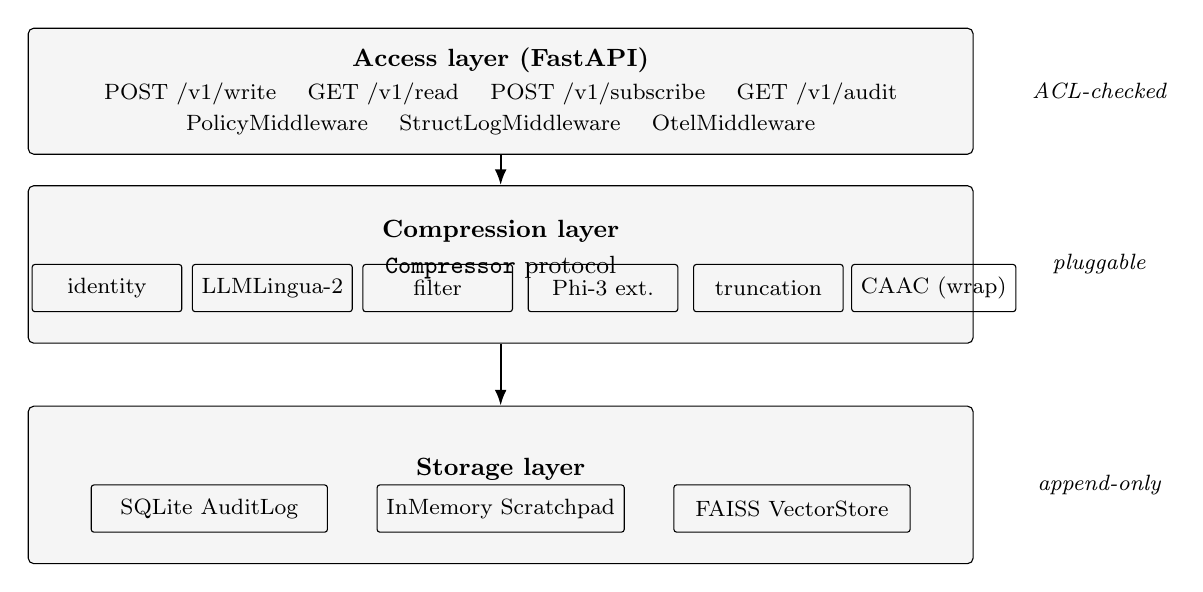
\begin{tikzpicture}[
    layer/.style={draw, rounded corners=2pt, minimum width=12cm,
                  minimum height=1.6cm, align=center, font=\small},
    cmp/.style={draw, rounded corners=1pt, minimum width=1.9cm,
                minimum height=0.6cm, font=\footnotesize},
    arrow/.style={-{Latex[length=2mm]}, thick},
    label/.style={font=\footnotesize\itshape}
]
% Access layer
\node[layer, fill=black!4] (access) at (0,4)
  {\textbf{Access layer (FastAPI)} \\[1pt]
   \footnotesize POST /v1/write \quad GET /v1/read \quad POST /v1/subscribe
   \quad GET /v1/audit \\
   \footnotesize PolicyMiddleware \quad StructLogMiddleware \quad OtelMiddleware};

% Compression layer
\node[layer, fill=black!4, minimum height=2.0cm] (compress) at (0,1.8)
  {\textbf{Compression layer} \\[2pt]
   \texttt{Compressor} protocol \\[2pt]};
\node[cmp] (id)     at (-5.0, 1.5) {identity};
\node[cmp] (lingua) at (-2.9, 1.5) {LLMLingua-2};
\node[cmp] (filter) at (-0.8, 1.5) {filter};
\node[cmp] (phi)    at ( 1.3, 1.5) {Phi-3 ext.};
\node[cmp] (trunc)  at ( 3.4, 1.5) {truncation};
\node[cmp] (caac)   at ( 5.5, 1.5) {CAAC (wrap)};

% Storage layer
\node[layer, fill=black!4, minimum height=2.0cm] (storage) at (0,-1.0)
  {\textbf{Storage layer} \\[2pt]};
\node[cmp, minimum width=3cm] (audit) at (-3.7, -1.3) {SQLite AuditLog};
\node[cmp, minimum width=3cm] (scr)   at ( 0.0, -1.3) {InMemory Scratchpad};
\node[cmp, minimum width=3cm] (vs)    at ( 3.7, -1.3) {FAISS VectorStore};

% Arrows between layers
\draw[arrow] (access) -- (compress);
\draw[arrow] (compress) -- (storage);

% Side annotations
\node[label] at (7.6,  4.0) {ACL-checked};
\node[label] at (7.6,  1.8) {pluggable};
\node[label] at (7.6, -1.0) {append-only};
\end{tikzpicture}
\caption{Three-layer architecture of the memory-bus reference
implementation. Each layer depends only on the layer below it, and
each storage component is hidden behind a \texttt{Protocol} so that
the storage backends can be replaced without touching the access or
compression layers. CAAC is drawn inside the compression layer for
convenience but is a wrapper: it composes any of the other
compressors with a recall-side back-off rule
(Section~\ref{sec:compressors_caac}).}
\label{fig:architecture}
\end{figure}

The three-layer structure is a direct extension of
MemIndex~\cite{saleh2025memindex}, the FCG group's baseline architecture
for distributed agent memory. The two material differences are that
compression is promoted to a first-class layer rather than treated as
a downstream optimisation, and that per-slot tags are part of the
data model rather than out-of-band metadata.

\subsection{Data flow for a write}

A \texttt{POST /v1/write} carries the fragment text, its tag vector,
and an optional task hint. The policy middleware parses the principal
from the \texttt{X-M6-Principal} header and checks that its
access-control mask is a superset of the fragment tag's and its
classification at least the fragment's. On success the service
compresses the fragment to a \texttt{CompressedSlot}, stores it in
the scratchpad, adds any embedding to the FAISS index, and appends a
\texttt{WRITE}/\texttt{OK} audit row whose
$\texttt{chain\_hash}=\textsc{SHA-256}(\texttt{prev\_hash}\mathbin\Vert\texttt{payload\_hash})$;
the response returns the slot id, hex chain hash, and audit row id. A
failed check appends a \texttt{DENY} row (slot \texttt{deny-<uuid8>})
with a $60$-second per-(subject, fragment-id) deduplication so a
client hammering denied writes cannot inflate the log.

\subsection{Data flow for a read}

A \texttt{GET /v1/read/\{slot\_id\}} flows symmetrically: the
middleware attaches the principal, the service looks up the slot,
checks the principal--tag relationship, and either returns the slot
with its audit row id or raises a policy-denied / slot-not-found
error. Read misses are audited as \texttt{READ}/\texttt{ERROR} rows
with the same $60$-second per-(subject, slot-id) deduplication.
Appendix~\ref{appendix} gives an end-to-end \texttt{curl} trace.

\subsection{Tags, classifications, and the audit log}

Every fragment and every compressed slot carries a tag vector
recording its provenance and access-control state. The tag vector has
four fields: a \texttt{uint64} access-control mask, a five-tier
classification level (\textsc{public} $<$ \textsc{internal} $<$
\textsc{confidential} $<$ \textsc{restricted} $<$ \textsc{secret})
drawn from enterprise data-classification practice (e.g., ISO/IEC 27001
organisational schemes); the broader risk-management framing follows
the NIST AI Risk Management
Framework~\cite{nistairmf}, but the five-tier lattice itself is
enterprise convention and not prescribed by NIST AI RMF (which
defines Govern/Map/Measure/Manage functions rather than a
labelled classification lattice). The remaining two fields are a
tuple of source identifiers recording provenance and a tuple of
parent-slot identifiers recording which previously-compressed slots
this slot inherits from. When slots are
merged, the union's access-control mask is the bitwise OR of the
parents' masks and the union's classification is the maximum; the
policy predicate is symmetric for reads and writes.

The audit log is an append-only SQLite table; each row records the
\texttt{event\_type} (WRITE/READ/SUBSCRIBE/DENY/COMPRESS/EVICT),
\texttt{slot\_id}, requester ACL mask and classification, result, and
a tamper-evident hash chain
($\texttt{chain\_hash}=\textsc{SHA-256}(\texttt{prev\_hash}\mathbin\Vert\texttt{payload\_hash})$).
An \texttt{INSTEAD OF UPDATE} and an \texttt{INSTEAD OF DELETE}
trigger refuse any mutation of an existing row, and a unit test drops
the trigger, edits a \texttt{payload\_hash} at the byte level, and
confirms that the \texttt{verify()} chain-walker reports failure.

A second SQLite table records every paid model call (provider,
model, token counts, EUR cost, wallclock), sharing the audit database
for transactional consistency. Pricing follows a representative
frontier rate (Anthropic Claude Sonnet tier, USD~$3$/$15$ per million
input/output tokens, $\approx$
EUR~$2.76$/$13.80$ at $0.92$~USD/EUR) against an on-premises marginal
$\approx$ EUR~$0.05$ per million tokens~\cite{fcgfinancial2026}; the
ledger feeds the EUR-per-workflow cost model of the RAG catalogue
(Section~\ref{sec:rag_pipelines}).

\section{Retrieval-Augmented Generation Pipeline Catalogue}
\label{sec:rag_pipelines}

The H3 analysis (Appendix~\ref{appendix:rag}) compares three
pipeline placements over the shared FAISS-CPU + HNSW +
\texttt{bge-large-en-v1.5} stack: \textbf{P1} compress-first
(compress the corpus, then index it), \textbf{P2} retrieve-first
(index the full corpus, then compress the top-$k$, the classical
LongLLMLingua~\cite{jiang2024longllmlingua} configuration), and
\textbf{P3} a joint relevance router (pass high-scoring fragments
verbatim, compress mid-scoring, discard low-scoring; after
ACC-RAG~\cite{guo2025dynamic}). Because the pre-specified sign-flip
did not appear and the cost model does not meter compression compute,
H3 is reported as a secondary result in Appendix~\ref{appendix:rag}.

\section{Compressor Framework}
\label{sec:compressors}

Every compressor variant conforms to a single Python \texttt{Protocol}
with four methods: \texttt{compress(fragment, target\_ratio)}
returning a \texttt{CompressedSlot}; \texttt{decompress(slot)}
returning a best-effort text reconstruction; \texttt{embed(slot)}
returning an optional embedding for vector-store indexing; and
\texttt{model\_card()} returning a structured card containing the
compressor identifier, family, base model, default target ratio, and
provenance hashes. The thesis ships six concrete implementations.
The identity compressor is the no-compression control that every
experiment needs to guard against runtime-bug confounds.

The remaining five compressors fall into four families: a
token-level hard-prompt filter (LLMLingua-2); an instruction-aware
heuristic filter; an extractive small-LLM span selector
(Phi-3-Mini extractive); a trivial prefix-truncation baseline; and a
cliff-aware adaptive wrapper (CAAC). \emph{All five are
training-free}, which is a deliberate design choice: the thesis
isolates the compression mechanism from any training-data effect
and lets the cross-compressor comparison turn on the algorithm
rather than on training-budget asymmetry.

\subsection{LLMLingua-2 (token-level classifier)}

The LLMLingua-2 wrapper is a thin adapter around the
\texttt{llmlingua} package~\cite{pan2024llmlingua2}. Construction
takes a target compression ratio; the package is asked to retain
$1/r$ of the tokens, scored by a small XLM-RoBERTa classifier
distilled from a more capable teacher. The force-tokens list
(sentence boundary marks) is validated against the wrapped
tokenizer's vocabulary at initialisation and unknown tokens are
dropped with an explicit log line. PyTorch runs the wrapped
XLM-RoBERTa model on both CPU and Apple's Metal Performance Shaders
backend, so the compressor runs natively on Apple Silicon without
modification.

The empirical token-recall curve $q(r)$ produced by LLMLingua-2
under critical-token-recall measurement (Section~\ref{sec:ctr})
is smooth and monotonic across the sweep ratios used in
\charef{experiments}, which is the property the
compounding-error model presumes.

\subsection{Instruction-aware filter}

The instruction-aware filter is a pure-Python heuristic baseline.
It operates in two stages. The first is a sentence-level filter
that ranks sentences by their relevance to the task hint using a
cross-encoder reranker (\texttt{BAAI/bge-reranker-base}) when
available and a lexical-overlap fallback when not. The second is a
token-level trim that drops English stop-words and short tokens
($\le 2$ characters) until the target compression ratio is reached.
The stop-word list is encoded explicitly so that the trim is
deterministic given the task hint, the fragment, and the target
ratio: a subtle bug showed that dropping stop-words in Python
set-iteration order introduced run-to-run variance.

The filter's reranker preserves task-keyword tokens that simpler
token-level methods drop, which is why its $q(r)$ curve on the
multi-step retrieval family (Section~\ref{sec:c1}, family-c) decays
gracefully rather than collapsing: chain-reference tokens like
``entry'' and ``FINAL'' survive aggressive compression.

\subsection{Phi-3-Mini extractive span selector}
\label{sec:phi3}

The Phi-3-Mini extractive compressor is the only thesis compressor
that uses an LLM at inference time. It runs the Phi-3-Mini-3.8B
instruction-tuned model~\cite{phi3} via a local Ollama
endpoint~\cite{ollama} with a structured prompt that asks for
verbatim contiguous spans from the source. The post-hoc verifier
\texttt{Phi3ExtractiveCompressor.\_verify\_extractive} checks the
output: every token in the output must appear in the source. Two
loosenings of the strict verifier were necessary in practice. First,
a $15\%$ novel-token tolerance: small language models frequently
insert function words (``the'', ``is'', ``and'') even when
explicitly asked not to. Second, a post-hoc
\texttt{\_strip\_novel\_tokens} pass that removes any token not in
the source after the verifier passes; this guarantees zero novel
tokens in the final output even if the model produced some during
generation. Outputs that fail even after stripping fall back to
LLMLingua-2 at the same target ratio.

Phi-3-Mini extractive has a \emph{compression ceiling}: span-level
selection, the stripping pass, and the LLMLingua-2 fallback together
bound the achievable ratio at about $2.5\times$, regardless of the
requested target. This is documented as a limitation in
\charef{summary} and is the reason all evaluation reports
\emph{achieved} compression ratio (the ratio actually delivered)
alongside the requested target ratio.

\subsection{Truncation (prefix-keep baseline)}

The truncation compressor keeps the first $1/r$ fraction of tokens
by whitespace split. It is deterministic by construction and
achieves the requested ratio exactly. Its purpose is the
lower-bound argument: every more sophisticated compressor must
beat truncation on the coordination metric to justify its cost.

Truncation has a peculiar property: its single-agent
question-answering F1 is competitive with the more sophisticated
compressors at low to moderate compression ratios because the
prefix tokens are naturally representative. Its coordination
success collapses earlier than the others, because the tokens
removed at the tail include the task-critical content that the
planner needs to combine. This dissociation is part of the H1
finding: a token-overlap quality metric over-reports the utility
of even the most naive compressor.

\subsection{Cliff-Aware Adaptive Compression (CAAC)}
\label{sec:compressors_caac}

CAAC is a wrapper, not a fifth compressor family. Given an inner
compressor (LLMLingua-2 in the headline experiments; any of the
others in the ablation) and a per-family recall threshold
$\theta_q$, CAAC runs the inner compressor at the requested target
ratio, measures the resulting critical-token-recall, and if recall
falls below $\theta_q^{1/N}$ binary-searches downward for the
largest ratio that keeps recall above the threshold. A
\texttt{min\_ratio} floor of $1.5\times$ prevents CAAC from
abdicating to no-compression on hard fragments. The full
algorithmic and empirical discussion lives in
\charef{summary} together with the constructive framing
that CAAC is the operational realisation of the compounding-error
bound. Here it suffices to note that CAAC consumes the same
\texttt{Compressor} protocol as the other variants, which is what
makes its drop-in evaluation in \charef{experiments}
straightforward.

\section{The C1 Coordination Benchmark}
\label{sec:c1}

\subsection{Why a synthetic benchmark}

The coordination cliff $\tau^{*}$ is a position on a curve, and
detecting it requires sweeping ratios densely from $1\times$ to
$16\times$ with everything else held constant. Real benchmarks
(HotpotQA, MultiHop-RAG) confound the cliff with task difficulty,
retrieval distribution, and per-instance variance, so the thesis
characterises the cliff on a synthetic generator first (where
information density is placed by construction) and validates the
transfer on real benchmarks (Corollary~2). The C1 generator produces
$150$ instances across three families from a single seed, with the
config hash recorded in the manifest so any output CSV traces back to
its generator inputs.

\subsection{Three workload families}
\label{sec:c1_families}

\begin{description}\setlength\itemsep{2pt}

\item[Family-a: cross-document fact aggregation.] Eight source
documents, one per Vignette~3.7 institutional
system~\cite{fcgusecase2026}, each carrying a recorded-hours and an
approved-budget number from a seed-fixed distribution; the planner
aggregates both across the eight, scored by a regex extraction
pipeline against the deterministic arithmetic sum. Family-a is the
densest ($\theta_\text{info}\approx0.97$): every multi-digit number
is task-critical and the cliff is sharp, so it is where the
compounding-error model is most directly testable.

\item[Family-b: constraint-satisfaction planning.] $N$ sub-tasks
with per-task loads and $K$ capacity-bounded workers; the planner
must assign every sub-task within capacity. The generator guarantees
at least one feasible assignment (capacity-respecting greedy), and
the scorer is a \emph{feasibility checker}: any valid assignment
scores~$1$. Constraint tracking is hard for $\le8$B planners even
without compression, so the family-b baseline $p_0$ is low for small
planners and the cliff is undetectable there: a \emph{floor effect}
\charef{experiments} treats explicitly.

\item[Family-c: multi-step retrieval.] A linear chain of fragments,
each carrying a pointer to the next (\emph{entry~X}) or, at the leaf,
the answer (\emph{FINAL-XXXX}); chain lengths $2$--$4$, padded with
$4$--$8$ distractor sentences, scored against the leaf answer.
Family-c is the most distributed of the three: many tokens are distractors,
information density $\theta_\text{info}\approx 0.62$ (distinct from the recall
threshold $\theta_q$; see Section~\ref{sec:theta_info_def}), and the
cliff is gradual; it is the family on which the instruction-aware
filter's reranker, which preserves chain-reference keywords, can
avoid a detectable cliff entirely.
\end{description}

Each family contributes $50$ instances. The three families together
span a deliberate range of information densities so that the cliff
mechanism (a recall threshold $\theta_q$) and the cliff-position
shift mechanism (information density $\theta_\text{info}$) can be
separated; this separation is what \charef{experiments}
formalises as Corollary~2.

\subsection{Tag distributions for the privacy axis}

The C1 generator supports three synthetic tag distributions
(\emph{uniform}, \emph{skewed}, \emph{hierarchical}) used by H4 to
probe the governance-stringency dimension. The hierarchical
distribution sets higher classification levels to imply strict
supersets of the lower-level bits, matching enterprise tag
hierarchies and letting H4 disentangle classification level from
access-control mask.

\subsection{Coordination success and supporting metrics}

The coordination scorer is a pure function of the workload and the
planner's output; it does not call any LLM. It returns one primary
metric (a per-instance binary \emph{coordination success}) and
four supporting metrics: the F1 over extracted answer tokens versus
ground truth, the achieved compression ratio
($|\text{source}|/|\text{compressed}|$), generic token-recall (the
fraction of source tokens preserved in the compressed text), and
\emph{critical-token-recall} (CTR; Section~\ref{sec:ctr}).
Aggregation across workloads $\times$ seeds is by arithmetic mean;
$95\%$ confidence intervals are computed by workload-level
bootstrap, never by per-row bootstrap which double-counts the seed
dimension.

The reason the scoring pipeline never calls an LLM is the same
reason H1 and H2 use a deterministic regex parser as the planner:
isolating the compression-quality signal from LLM run-to-run
variance. The trade-off is that the cliff measured here is an upper
bound on what an LLM-based scorer would measure; the trade is in
favour of clean attribution rather than ecological validity, and
\charef{summary} discusses the limitation.

\subsection{The critical-token-recall metric}
\label{sec:ctr}

A standard token-recall measurement
$q_\text{token}(r) = |T_\text{compressed} \cap T_\text{source}| /
|T_\text{source}|$ counts every preserved token equally. This proved
a poor proxy for task-relevant information preservation: the
Phi-3-Mini extractive compressor at low ratios preserves common
function words like ``the'' and ``and'' but drops some critical
numeric tokens. Its token-recall is high; its coordination success is low.

The critical-token-recall (CTR) metric is the family-specific
restriction:
\[
  q_\text{CTR}(r) = \frac{|T_\text{compressed}^{\,\text{crit}} \cap
                          T_\text{source}^{\,\text{crit}}|}
                         {|T_\text{source}^{\,\text{crit}}|},
\]
where $T^\text{crit}$ is the set of \emph{task-critical} tokens for
the family:
\begin{itemize}\setlength\itemsep{1pt}
\item Family-a: multi-digit numeric tokens (at least two digits, to
exclude single-digit noise);
\item Family-b: all numeric tokens (load and capacity values);
\item Family-c: chain-reference tokens (\emph{entry-X} patterns) and
the literal \emph{FINAL} marker.
\end{itemize}

CTR is what the compounding-error model uses as the per-round
retention rate $q(r)$; CAAC uses CTR as its back-off signal; and
the predicted-versus-empirical $\tau^{*}$ figure in
\charef{experiments} uses CTR to derive $\theta_q$. Generic
token-recall is reported for backwards compatibility with prior
analyses but is not used in the verdict pipeline.

\section{Compression Cache}
\label{sec:cache}

Compression is the slowest evaluation step (Phi-3-Mini extractive
is a $\sim11$~second Ollama call per fragment), and the cliff sweep
touches $\approx30{,}000$ (compressor, ratio, workload, task-hint)
cells, so a precomputed cache (\texttt{CompressionCache} /
\texttt{CachedCompressor} in \texttt{src/m6/compressors/cache.py},
keyed on
$(\text{compressor}, r, \text{fragment\_id}, \text{hash}(\text{task\_hint}))$)
is populated once on the GPU and consumed as JSON thereafter. This
decouples compression from evaluation, letting H1, H2, the frontier
sweep, and the CAAC ablation run on a laptop, and guarantees every
run sees identical compressed text for a cell, so run-to-run
differences are protocol, not compressor stochasticity (cache hit
rate $100\%$ by construction).

\section{Inference Backends}
\label{sec:inference}

The unified \texttt{InferenceBackend} protocol exposes a single
\texttt{complete(prompt, max\_tokens, temperature, stop)} method
together with an optional \texttt{embed(text)} method. Three concrete
backends are used in the evaluation. The first is a local Ollama
endpoint~\cite{ollama} that hosts Qwen-2.5-Instruct at the three
local sizes (\textsc{1.5B}, \textsc{3.8B}, \textsc{8B}) used in
the model-scaling sweep, Phi-3-Mini-3.8B for the extractive
compressor, and Llama-3.1-8B-Instruct~\cite{llama31modelcard} as the
local protected-fact reader. The second is the OpenAI-compatible Featherless API used
for the frontier validation (Qwen-2.5-72B-Instruct, DeepSeek V4
Pro). The third is the OpenAI API for the GPT-class frontier
arm (excluded from the calibrated regime per
\charef{summary}, retained on disk as a noncanonical
diagnostic). All API calls are routed through the cost ledger so
that the EUR-per-workflow figures in
\charef{experiments} are auditable.

\section{Design Choices and Alternatives Considered}
\label{sec:design_choices}

The artefacts above are not a default stack; each tool and parameter
was a choice with a credible alternative, catalogued here so the
results of \charef{experiments} can be read against the decisions
that made them. The per-hypothesis falsifiability bars are discussed
at the point of pre-specification
(\charef{experiments}~Section~\ref{sec:prereg_refinement}).

\subsection{Tooling: storage, retrieval, and serving stack}
\label{sec:design_tooling}

The serving stack is chosen for single-host reproducibility:
\textbf{FAISS-CPU}~\cite{faiss} with an HNSW index (over Qdrant/Chroma/pgvector)
so the reference service ships as one Docker image with no external
database and no GPU dependency for retrieval;
\texttt{BAAI/bge-large-en-v1.5} embeddings with a
\texttt{bge-reranker-base} re-ranker (open-weight, digests in
\texttt{docs/MODEL\_CARDS.md}); \textbf{FastAPI}/Starlette for the
access layer; \textbf{SQLite-WAL} for the audit log (one-file
footprint, concurrent reader--writer, a replicated multi-host chain
named as future work); \textbf{Ollama} for local LLM serving
(uniform model lifecycle across the Apple-Metal and CUDA hosts behind
one \texttt{complete()} call, Section~\ref{sec:inference}); and the
OpenAI-compatible \textbf{Featherless} endpoint for the frontier arm,
chosen for its flat per-token price so the EUR cost model compiles
without per-provider markup tracking.

\subsection{Compressors considered but not swept}
\label{sec:design_compressors_declined}

Three compressor families from the survey were considered and
excluded, recorded so the omissions are deliberate.
\textbf{Selective Context}~\cite{li2023selective} requires a scoring
forward pass at compression time (asymmetric compute with the swept
four) and its design point (task-aware lexical pruning with no
end-to-end LM) is already covered by the instruction-aware filter.
\textbf{RECOMP}~\cite{xu2024recomp} and \textbf{learned compression}
(gist tokens~\cite{mu2023gist},
AutoCompressor~\cite{chevalier2023autocompressor},
ICAE~\cite{ge2024icae}) require fine-tuning, which would confound the
deliberately training-free cliff comparison with training-budget
asymmetry (re-evaluating them is named as follow-on work).
\textbf{xRAG}~\cite{cheng2024xrag} represents a document as a single
token ($>100\times$), beyond the $1$--$16\times$ regime where the
cliff sits. For the extractive compressor's base model, Phi-3-Mini
was chosen over Llama-3.2-3B and Mistral-7B on pilot
extractive-verifier pass rates ($\sim 75\%$ vs
$\sim 62\%$/$\sim 71\%$ pre-fallback) at the smallest deployment
footprint.

\subsection{Threshold and sweep-grid parameters}
\label{sec:design_thresholds}

The cliff measurement turns on a few numerical parameters. The
\textbf{ratio grid} $\{1,2,3,4,5,6,8,10,12,16\}\times$ is denser at
the low end where the dense-family cliff sits; a fine-grid
re-resolution (\charef{experiments}~Section~\ref{sec:h2}) later
showed the $r\in\{1,2\}$ gap is itself too coarse for the
deterministic-solver family-a cliff near $r=1.1$, with
$\mathbf{r_{\max}=16}$ because beyond it every compressor's CTR is
near zero on family-a. \textbf{$50$ instances per family, $5$ seeds
per cell} ($250$ pairs per cell) is the smallest sample at which the
workload-level bootstrap CI clears the H1/H2 bands at the budgeted
compute; there is no formal a-priori power analysis, named as a
limitation in \charef{summary}. \textbf{$\theta_q$ at
$0.5\times p_0$} reads off ``coordination has collapsed'' without a
separate calibration sweep and sits below the H2 $30\%$-drop bar; the
CAAC ablation finds the coordination plateau invariant to
$\theta_q\in\{0.6,0.7,0.8\}$. The \textbf{bootstrap} uses BCa
intervals~\cite{efron1993bootstrap} at $n_\text{boot}=10{,}000$ on
the verdict pipelines and $500$ on the $\theta_q$ and
frontier-$\tau^{*}$ pipelines, whose per-iteration curve fit is the
budget driver.


\section{Scope of Evaluation: the Multi-Fragment Proxy}
\label{sec:scope}

The empirical protocol uses two planners, isolating the
compression-quality signal from LLM variance: a deterministic regex
information-extraction solver for H1/H2, and a single LLM call with
all compressed fragments visible for Corollary~1, the frontier
validation, and the real-data transfer (demonstrating that the cliff
structure the solver measures appears identically under a non-trivial
language model). The AutoGen v0.4 multi-round
backend~\cite{wu2023autogen} in \texttt{src/m6/orchestrator/}
integrates with the bus but is not used: multi-round negotiation
variance dominates the compression signal at the swept ratios, so the
backend demonstrates that the bus is multi-agent-ready rather than
serving as the measured planner. Coordination success
(Section~\ref{sec:c1}) is therefore the structural property that the
planner must combine information across fragments, not multi-round
communication quality, which \charef{summary} names as future work.

\section{Compute Envelope and Reproducibility}
\label{sec:envelope}

The empirical work runs on an Apple~M4~Pro 48~GB workstation (local
Ollama planners, deterministic-solver pipeline, and every figure when
the compression cache is in place) and an RTX~5090 32~GB host
(compression precompute, the $8$B model-scaling sweep, the frontier
API sweep, and the HotpotQA / MultiHop-RAG transfer). Total wallclock
for the canonical pipeline is $\sim 30$~GPU-hours plus $\sim 12$~hours
of laptop time. The reproducibility package is the complete
repository: a \texttt{docker-compose.yml} for the memory-bus
service, a release tag, model and data cards, and one-command
\texttt{make} targets for every headline figure; one CSV per
hypothesis run plus a \texttt{manifest.yaml} recording the resolved
configuration, the config hash, the git revision, and the platform.
Appendix~\ref{appendix} lists the commands and the full compute stack.


\chapter{Experiment Design and Protocol}
  \label{experiments}
  This chapter presents the empirical work that this thesis turns on:
the cliff sweep on which H1, H2, and the compounding-error model are
based; the model-scaling sweep whose result is reported as
Corollary~1; the frontier validation that promotes the
model-independence claim from small-model evidence to a
cross-architecture result inside a defined calibrated regime; the
retrieval-augmented-generation pipeline catalogue (H3); the
summary-level inference-disclosure measurement (H4); and the
information-density scaling result on real benchmarks reported as
Corollary~2. The chapter is organised around the falsifiable claims
rather than the chronology of the runs; canonical results directories
under \texttt{results/} are referenced for each section so that
every number is traceable to an immutable artefact on disk.

\section{Pre-specification and Refinement}
\label{sec:prereg_refinement}

The six investigations of this chapter were pre-specified with
falsifiable criteria in \texttt{configs/experiments/h\{1-6\}.yaml}
and \texttt{plan-v3.md}. The six hypotheses and the statistical
protocol were committed to the project repository on 2026-05-21,
prior to the data-generation runs that produced the headline
numbers reported in this chapter (the final sweeps ran from
2026-05-26 onward). This is a pre-specified protocol committed to
version control, not a third-party-frozen pre-registration
(e.g.\ OSF or AsPredicted). The criteria for H3, H5, and H6 were
refined after the sweeps; the refinements are documented as ADR-006--008
in the project repository. The three-tier structure used in the rest
of the chapter is as follows.

\textbf{Three hold as pre-specified.} H1 (workload-level
source-retention F1 does not transferably predict coordination
success), H2 (a sharp cliff
at \mbox{$\ge\!30$\%} drop with $p<0.05$ on \mbox{$\ge\!7/9$} cells),
and H4 (compression reduces inference disclosure with baseline above
priors).

\textbf{Two sharpened.} H5's monotonicity prediction resolved into
the invariance result \textbf{Corollary~1 (Ceiling--Cliff
Separation)}, Section~\ref{sec:corollary1}: $\tau^{*}$ is determined
by the compressor and the task within a calibrated regime, while
planner scale moves the ceiling $p_0$. H6's transfer prediction
resolved into \textbf{Corollary~2 (Information-Density Scaling)},
Section~\ref{sec:corollary2}: the cliff position varies with task
information density $\theta_\text{info}$.

\textbf{One narrowed.} H3's regime sign-flip predicate
($\ge\!5$~pp F1 effect with opposite sign across storage- and
accuracy-bounded regimes) is not satisfied; compress-first dominates
on the tested stack in both regimes (Section~\ref{sec:h3}).

\subsection{Falsifiability criteria as practitioner-relevant minima}
\label{sec:prereg_criteria_defense}

Each numerical bar above ($\rho<0.6$ for H1, $\ge 30\%$ drop for H2,
$\pm 5$~pp F1 sign-flip for H3, paired-bootstrap $p<0.05$ for H4,
$\pm 20\%$ TOST band for Corollary~1, $\Delta\theta_\text{info}
\ge 0.1$ for Corollary~2) was chosen as the smallest effect a
practitioner relying on this thesis would care about, not as an
arbitrary statistical threshold. The catalogue below makes the
rationale for each bar explicit; tool and grid choices (the
ratio grid, the bootstrap budget, the $\theta_q$-at-$0.5 \cdot p_0$
rule) live in \charef{implementation}~Section~\ref{sec:design_choices},
and metric choices in Section~\ref{sec:metric_choices} of this
chapter.

\begin{description}\setlength\itemsep{2pt}
\item[H1 ($\rho < 0.6$, workload-level).] Cohen's convention for
``less than moderate'' rank correlation. A compressor ranking with
$\rho \ge 0.6$ would remain operationally useful to a practitioner
who needs to deploy compression; clearing $\rho < 0.6$ from above
is the bar at which the predictive utility of the single-agent
F1 metric collapses. The verdict's reliance on the workload-level CI
(rather than the pooled CI) follows the unit decision in
Section~\ref{sec:metric_unit}.
\item[H2 ($\ge 30\%$ relative drop, Holm-corrected $p < 0.05$).]
$30\%$ is the smallest coordination-success drop a practitioner
cares about. A $10\%$ drop sits within typical run-to-run variance
on the families this thesis evaluates; a $50\%$ drop is obvious
without measurement; $30\%$ is the value below which the operating
point would still be deployable and above which it would not. The
Holm correction is applied within the $12$-cell family of
(compressor, family) pairs, not across hypotheses, because the H2
claim is internal to that family.
\item[H3 ($\ge 5$~pp F1 effect with opposite sign across regimes).]
$5$~pp F1 is the smallest gap the practitioner cost-model
(EUR-per-workflow, Section~\ref{sec:h3}) makes operationally
meaningful; opposite sign is what would justify regime-conditional
deployment of P1 versus P2 at all. The pre-specified predicate is
what the data did not support, which is the H3 narrative.
\item[H4 (paired-bootstrap $p < 0.05$, positive direction).]
Paired bootstrap because the same workloads appear in the
priors / baseline / compressed conditions; $p < 0.05$ is
conventional; the positive direction is the privacy direction
(compression must reduce, not increase, disclosure). The
construct-validity caveat in Section~\ref{sec:h4_construct} is
about the privacy \emph{interpretation} of a positive effect, not
about whether the effect itself is detectable.
\item[Corollary~1 ($\pm 20\%$ TOST equivalence band).]
The $\pm 20\%$ band is the strict cliff-position-detectability
tolerance reported alongside the $\pm 50\%$ permissive default in
\texttt{validate\_model\_independence}. The permissive band
absorbs the noise inherent in the local-model arm (small samples,
high run-to-run variance); the strict bar is the one a
deployment-grade ``no shift detected'' claim ought to clear, and
is the one the frontier-validation evidence is tested against. The two are
reported alongside each other in
Section~\ref{sec:corollary1}, and the strict bar is what
the on-disk record \texttt{model\_independence\_20pct.json}
quantifies.
\item[Corollary~2 ($\Delta\theta_\text{info} \ge 0.1$ between
dense and distributed benchmarks).]
$0.1$ is the smallest information-density gap that produces a
qualitatively distinct cliff shape on the three benchmarks
evaluated --- below this gap the cliffs are visually
indistinguishable on the AUC-based $\theta_\text{info}$ axis. The
bar is conservative against estimator noise: the empirical gaps in
Table~\ref{tab:corollary2} ($0.48$ between C1 family-a and
MultiHop-RAG, $0.59$ between C1 family-a and HotpotQA) clear it by
several multiples, so the corollary verdict does not turn on the
precise location of the bar within the noise floor.
\end{description}

The motivation for surfacing these defences here is that an
external reviewer will reasonably ask why a particular threshold
was chosen; each one is defensible as a practitioner-relevant
minimum, not an arbitrary statistical choice.

The consolidated table is Table~\ref{tab:verdict_summary}
(Section~\ref{sec:verdict_summary}).

\section{Experimental Protocol}
\label{sec:protocol}

\subsection{The cliff sweep}

The cliff sweep underlies H1, H2, and the calibration step of the
compounding-error model. Four compressors --- LLMLingua-2,
Phi-3-Mini extractive, the instruction-aware filter, and a
truncation baseline --- are evaluated at ten compression ratios
$\{1, 2, 3, 4, 5, 6, 8, 10, 12, 16\}\times$ on the $150$ C1
workloads across the three families. Five seeds per cell give a
total of approximately $30{,}000$ evaluation cells per run. The
canonical results directory is
\texttt{results/h1\_h2\_v2/}; the earlier
three-compressor variant \texttt{results/h1\_h2\_final/} is retained
on disk for backwards-compatibility checks but is not the source of
the headline numbers below. The truncation baseline is the
lower-bound argument: any compressor that does not beat truncation
on the coordination metric is paying training or inference cost for
no coordination-quality return.

Every cell records the coordination-success binary, the
source-retention F1 (token-overlap F1 between the compressed
fragments and the original source text --- the \texttt{qa\_f1}
column H1 analyses, \emph{not} answer-level QA-F1 against a gold
answer), the achieved compression ratio, the
generic token-recall, and the critical-token-recall described in
Section~\ref{sec:ctr} of \charef{implementation}. The
compression cache (Section~\ref{sec:cache}) guarantees that every cell
sees the exact same compressed text for a given (compressor, ratio,
workload) tuple, so within-cell variance is exclusively
planner-side variance, not compressor stochasticity.

\subsection{Statistical protocol}
\label{sec:stats}

The statistical protocol is fixed in advance for every hypothesis.
Effect-size summaries are computed at the workload level, never
the cell level: per-workload means are computed first, and the
$95\%$ bootstrap confidence intervals are constructed by resampling
workloads with replacement~\cite{efron1993bootstrap}, never by
resampling individual seed--cell pairs. The bootstrap method is the
bias-corrected and accelerated (BCa) interval (per the construction in~\cite{efron1993bootstrap})
with $n_\text{boot} = 10{,}000$ resamples on the main H1/H2/H3/H4
verdict pipelines (the per-method defaults of
\texttt{spearman\_with\_ci}, \texttt{paired\_bootstrap\_diff}, and
\texttt{paired\_bootstrap} in \texttt{src/m6/}). The $\theta_q$
resampling pipeline of Section~\ref{sec:cem_match} and the
frontier-$\tau^{*}$ bootstrap of Section~\ref{sec:frontier} run at
$n_\text{boot} = 500$ instead, because both involve repeated curve
fits whose per-iteration cost is substantially higher than a
single-statistic resample. The two-cell comparison
test is the paired Wilcoxon signed-rank
test~\cite{wilcoxon1945}, chosen over the Mann--Whitney $U$
test~\cite{mannwhitney1947} because the same workloads appear in
both conditions, which violates the independence assumption of the
two-sample test. Multiple-comparisons correction is Holm's
sequentially-rejective procedure~\cite{holm1979bonferroni} applied
\emph{within each hypothesis's family}: the $12$ (compressor,
family) cells of the cliff sweep are Holm-corrected jointly for H2;
the three condition pairs of H4 are Holm-corrected jointly for the
disclosure signal and again jointly for the disclosure reduction;
the three pipelines of H3 are Holm-corrected jointly per regime.
Family sizes are deliberately kept narrow because the hypotheses
are independent claims and joint correction across them would be
over-conservative.

The H1 verdict statistic is the \emph{workload-level} Spearman
correlation ($n = 150$ workloads, one mean $\Delta$-pair per
workload, for every compressor; Phi-3-Mini extractive's
$\sim 2.5\times$ achievable-compression ceiling collapses the
upper ratio range and therefore reduces its \emph{pooled} $n$
from $150 \times 9 = 1350$ to $150 \times 5 = 750$, but does not
reduce the workload-level $n$, Section~\ref{sec:phi3}). A pooled
correlation over $n = 150 \times 9$ (workload, ratio) measurements
would over-state significance by roughly an order of magnitude,
because the nine per-workload ratios are repeated measures rather
than independent draws; that pooled $n$ and its asymptotic
$p$-value are therefore retained in Table~\ref{tab:h1_rho} only
as a non-inferential comparison column. The two-tailed asymptotic
$p$ for $H_0: \rho = 0$ is reported at the workload level; the
verdict rests on the BCa bootstrap CI (over workloads) excluding
$0.6$.

Cliff position $\tau^{*}$ is extracted by fitting both a piecewise-%
linear model and a logistic
\[
  f(r) = p_0 + \frac{p_\infty - p_0}{1 + e^{-k(r - \tau^{*})}}
\]
to each cell's coordination-success-versus-ratio curve and selecting
the model with the lower root-mean-squared error. The piecewise fit
is constrained to an interior $10\%$ margin from the sweep
boundaries. This prevents the optimiser from parking $\tau^{*}$ at
$r_{\max}=16$, a degenerate fit the unconstrained optimiser would
otherwise select. $95\%$~bootstrap CIs on $\tau^{*}$ are computed by
resampling the underlying workload means before the curve fit.

\section{Choice of Evaluation Metrics}
\label{sec:metric_choices}

Every metric reported in this chapter is a choice: a different
metric --- in some cases a more conventional one --- would have
produced a different verdict. This section catalogues all metrics
used in the chapter, names the alternative considered and the
reason it was declined, and consolidates the workload-level versus
cell-level statistical-unit decision that the H1 verdict in
particular turns on. The justification for each individual
hypothesis's falsifiability bar (the $\rho < 0.6$ bar for H1, the
$\ge 30\%$ drop for H2, etc.) is in
Section~\ref{sec:prereg_refinement}; this section is about the
choice of metrics themselves, not the cutoffs. Tool-side and
sweep-grid choices --- the ratio grid, the bootstrap budget, the
P3 routing thresholds --- live in
\charef{implementation}~Section~\ref{sec:design_choices}.

\subsection{Catalogue of metrics}
\label{sec:metric_catalogue}

Table~\ref{tab:metric_choices} enumerates the metrics by the point
at which they enter the verdict pipeline. The chapter's verdict
block in each section
($\!$Sections~\ref{sec:h1}--\ref{sec:corollary2}) rests on the
metrics in this table.

{\small
\begin{longtable}{p{3.0cm}p{5.4cm}p{5.4cm}}
\caption{Choice of evaluation metrics. ``Why chosen'' captures the
property each metric measures; ``Alternative declined'' names the
closest competitor and the reason it was not used.}
\label{tab:metric_choices} \\
\hline
Metric & Why chosen & Alternative declined \\
\hline
\endfirsthead
\hline
Metric & Why chosen & Alternative declined \\
\hline
\endhead
\hline
\multicolumn{3}{r}{\textit{(continued on next page)}} \\
\endfoot
\hline
\endlastfoot
\multicolumn{3}{l}{\textit{Task-level outcomes.}} \\
Coordination success (binary per-instance)
  & Directly answers ``did the planner recover the correct answer?'';
    matches the practitioner's deployment question and operationalised
    once in \charef{introduction}~Section~\ref{sec:multi_fragment}.
  & Graded success: the A3 probe (Section~\ref{sec:a3_probe}) shows
    binary is justified on dense tasks; the graded refinement is
    named as future work on distributed tasks. \\
Token-overlap F1 (qa\_f1)
  & Comparability to the LongLLMLingua / LLMLingua-2 numbers; the
    metric the prior literature reports against, which is what makes
    the H1 mis-ranking claim meaningful.
  & ROUGE-L: rewards long spans, less discriminating at high
    compression. BERTScore: requires an embedding model in the metric
    pipeline, conflates compressor and metric quality. \\
\hline
\multicolumn{3}{l}{\textit{Compressor-side measurements.}} \\
Critical-token recall (CTR)
  & Family-specific information-preservation signal; what the
    compounding-error model's $q(r)$ measures, and what CAAC's
    back-off uses.
  & Generic token-recall: empirically misleading on Phi-3 (preserves
    ``the'', drops numerics; Section~\ref{sec:ctr} of
    \charef{implementation}). Retained as a reporting column only. \\
Achieved compression ratio
  & Phi-3-Mini extractive saturates at $\sim 2.5\times$; reporting
    only the requested target hides the ceiling and would mis-rank
    Phi-3 against the token-level compressors.
  & Target ratio only: misleads on Phi-3's high-ratio cells; would
    suggest Phi-3 cliffs the same way the token-level compressors do
    when in fact it never reaches their compression range. \\
\hline
\multicolumn{3}{l}{\textit{Statistics and uncertainty.}} \\
Spearman $\rho$ (H1)
  & Rank correlation; appropriate for monotone-but-not-necessarily-%
    linear relations between $\Delta$qa\_f1 and $\Delta$coord; robust
    to clamping at the coord $\in\{0, 1\}$ boundaries.
  & Pearson $r$: requires linearity, breaks at the boundaries.
    Kendall $\tau$: equivalent at $n=150$ but less commonly reported
    by downstream readers. \\
BCa bootstrap ($n_\text{boot}=10{,}000$ for H1/H2/H3/H4; $500$ for
$\theta_q$ and frontier-$\tau^{*}$ pipelines)
  & Bias-corrected and accelerated~\cite{efron1993bootstrap} handles
    the skewed residuals near $\tau^{*}$ that the interior-clamped
    piecewise fit produces; the lower budget on the curve-fit
    pipelines reflects per-iteration cost rather than a different
    methodological choice.
  & Basic percentile: under-covers in skewed residuals. Jackknife:
    less stable on the workload-level resample at $n=150$. \\
Paired Wilcoxon signed-rank
  & The same workloads appear in both conditions; paired structure
    violates the independence assumption of Mann--Whitney.
  & Mann--Whitney $U$: independence fails on paired workloads.
    Paired $t$-test: not robust to non-normal coord-success
    distributions (heavily zero/one-inflated near the cliff). \\
Holm sequentially-rejective
  & Less conservative than Bonferroni at the family sizes used
    ($3$--$12$ cells), preserving power on the cliff-existence
    claim.
  & Bonferroni: over-conservative at these family sizes.
    Benjamini--Hochberg: controls FDR rather than FWER, which is the
    wrong error rate for a cliff-existence verdict. \\
TOST equivalence test (Corollary~1)
  & Direct test of ``no shift $\ge X$'' rather than the
    affirming-the-null reading of CI-containment.
  & CI-containment alone: weak evidence when the CI is wide (as on
    DeepSeek V4 Pro, Section~\ref{sec:frontier_deepseek}). \\
\hline
\multicolumn{3}{l}{\textit{Derived quantities.}} \\
$\theta_q$ (cliff-recall threshold)
  & Per-family recall at which coord-success drops to $0.5 \cdot p_0$;
    estimated by \texttt{derive\_theta()}; the model's threshold
    parameter.
  & Per-task $\theta_q$: lifted to future work because per-family is
    the tractable first-order term. \\
$\theta_\text{info}$ (AUC-based info density)
  & Captures the curve's \emph{shape} (sharp vs gradual). Explicitly
    distinct from $\theta_q$
    (Section~\ref{sec:theta_info_def}).
  & Conditional entropy of answer given input: an external probe
    that would break Corollary~2's circularity; named as future
    work. \\
Disclosure rate (H4)
  & Fraction of yes/no protected-fact questions correctly recovered;
    directly auditable against a governance budget.
  & ROC-AUC: requires probabilistic outputs the Ollama reader does
    not expose reliably. Calibration error: not what the threat
    model in Section~\ref{sec:h4_threat} asks. \\
\end{longtable}
}

\subsection{Workload-level versus cell-level statistics}
\label{sec:metric_unit}

A single methodological decision sits behind every effect-size
figure in this chapter: the inference-valid statistical unit is
the \emph{workload}, not the (workload, seed) cell or the
(workload, ratio) pair. The reason is mechanical: the five seeds
on each (compressor, ratio, workload) cell are repeated measures
of the same underlying coordination event, and the nine ratios per
workload are repeated measures of the same underlying compressor
behaviour. Treating either as independent draws --- which a pooled
correlation or a pooled bootstrap would do --- inflates the
effective $n$ by roughly an order of magnitude and over-states
statistical significance.

The H1 verdict in particular illustrates this: as
Section~\ref{sec:h1} reports, two of the four compressors
(LLMLingua-2 and truncation) drop from a pooled
$\rho \approx +0.38$ at $n = 1350$ to a workload-level
$\rho \approx 0.03$ at $n = 150$. The verdict (all CIs exclude
$0.6$) holds in both views, but only the workload-level magnitudes
correspond to a relationship a practitioner could exploit. The
pooled column is reported as a non-inferential comparison only,
and the H1 verdict table carries this distinction in its caption.

\subsection{Coverage}
\label{sec:metric_coverage}

The metrics in Table~\ref{tab:metric_choices} are exhaustive for
the verdict pipeline: every numerical claim in this chapter
resolves to one of these metrics, evaluated by the statistical
protocol of Section~\ref{sec:stats}. Metrics that are deliberately
\emph{not} in the table --- BERTScore, conditional-entropy probes
of $\theta_\text{info}$, per-question reader calibration, ROC-AUC
variants of the H4 disclosure measurement --- are named at their
respective points in the chapter or in
\charef{summary}~Section~\ref{sec:future} as follow-on work. The
position the thesis takes is that a small, carefully-defended
metric set whose statistical assumptions are tested is more
defensible than a larger metric set whose individual choices are
not justified.

\section{H1: Single-Fragment Information Preservation Does Not Transferably Predict Coordination Success}
\label{sec:h1}

\begin{tcolorbox}[colback=black!4, colframe=black!50, sharp corners,
                  boxrule=0.4pt, boxsep=2pt, left=4pt, right=4pt,
                  top=2pt, bottom=2pt]
\textbf{H1.} Single-fragment information preservation under
compression is not a transferable predictor of multi-fragment
coordination success: workload-level
Spearman~$\rho(\Delta_\text{qa}, \Delta_\text{coord}) < 0.6$ for
every compressor, with $95\%$ bootstrap CIs excluding $0.6$ from
above. \textbf{Verdict: SUPPORTED.} The finding is most honestly
stated as \emph{source-retention F1 change does not positively
predict coordination change for any compressor at the workload level},
plus a methodological warning that pooled single-number correlations
are distorted. At the workload level (the inference-valid unit),
the instruction-aware filter is strongly negative
($\rho = -0.82$), Phi-3-Mini extractive moderately positive
($\rho = +0.32$), and LLMLingua-2 and truncation collapse to
near-zero ($\rho = +0.03$ and $+0.05$, CIs spanning zero) --- even
though the filter, LLMLingua-2, and truncation look more correlated
($|\rho| \approx 0.38$--$0.59$) when ratios are pooled. We
deliberately avoid the word ``decorrelate'' for the filter
($|\rho| = 0.82$ is a strong correlation), but for LLMLingua-2 and
truncation near-zero is exactly what the workload-level data show.
A per-family decomposition (Table~\ref{tab:h1_perfamily}) explains
both effects: within most (compressor, family) cells coordination
collapses uniformly across workloads, leaving no rank variance
(``degenerate''); the filter's strong overall negative value is a
\emph{between-family} artifact (within family-a it is only $-0.13$,
n.s.); and the single significant within-family relationship is
\emph{negative} (LLMLingua-2/family-c, $-0.46$). The pooled
positive correlations for LLMLingua-2 and truncation are thus
inflated by pseudo-replication and between-family pooling and must
not be read as evidence that source-retention F1 tracks coordination.
\end{tcolorbox}

\subsection{Result}

The H1 single-fragment metric is \emph{source-retention F1}:
token-overlap F1 between the compressed fragment representation and
the original source text (\texttt{single\_agent\_qa} in
\texttt{run\_h1\_h2.py}, reported in the \texttt{qa\_f1} column). It
is \emph{not} answer-level QA-F1 against a gold answer; it is the
single-fragment information-preservation proxy that stands in for
the single-agent quality metric the prompt-compression literature
optimises~\cite{jiang2024longllmlingua,pan2024llmlingua2}.
Table~\ref{tab:h1_rho} reports the Spearman correlation between the
change in source-retention F1 and the
change in coordination success under compression, at both the
workload level (the inference-valid unit) and pooled-over-ratios
(for comparison only). The signature finding is twofold. First,
the workload-level correlations span from $-0.82$ (filter) to
$+0.32$ (Phi-3-Mini extractive) and none reaches $0.6$, with
LLMLingua-2 and truncation sitting essentially at zero ($+0.03$,
$+0.05$). Second, the workload-level and pooled columns disagree
sharply: pooling the nine ratios per workload inflates LLMLingua-2
and truncation to $\approx +0.38$ --- a pseudo-replication
artifact, since the nine ratios on one workload are not
independent. The filter's strongly negative workload-level value
is the easiest to misread and is why this section opens with the
verdict: the filter's re-ranker preserves task-keyword tokens that
the token-overlap metric does not reward, so as the F1 metric goes
down the coordination metric can go \emph{up}. But the per-family
decomposition (Table~\ref{tab:h1_perfamily}) shows even this is a
between-family effect --- within any single family the filter's
relationship is weak or undefined. The robust H1 statement is the
negative one: token-overlap F1 change does not positively,
consistently predict coordination change for any compressor at the
workload level.

\begin{table}[h]
\centering
\caption{H1 verdict table. Spearman correlation between
$\Delta$~token-overlap F1 and $\Delta$~coordination success under
compression. The workload-level $\rho$ (one mean $\Delta$-pair per
workload, $n=150$) is the verdict statistic. The pooled column
($n=1350 = 150~\text{workloads} \times 9~\text{ratios}$) is shown
for comparison only and is \textbf{not} used for inference: the
nine per-workload ratio measurements are repeated measures, not
independent draws, so the pooled $n$ and its asymptotic $p$
over-state significance by roughly an order of magnitude. The
verdict (all CIs exclude $0.6$) holds in both columns. CI is
BCa-bootstrap over workloads, $n_\text{boot}=10{,}000$ resamples
(\texttt{spearman\_with\_ci} default). Phi-3-Mini
extractive saturates at $\sim 2.5\times$ achieved compression so
its pooled $n$ is $750$ ($150 \times 5$); see
Section~\ref{sec:phi3} and Appendix~B.}
\label{tab:h1_rho}
\small
\begin{tabular}{p{3.4cm}rlr}
\hline
Compressor & $\rho$ (workload, $n$) & $95\%$ CI (workload) & $\rho$ (pooled, $n$) \\
\hline
Instruction-aware filter & $-0.818$ ($150$) & $[-0.852, -0.760]$ & $-0.593$ ($1350$) \\
LLMLingua-2              & $+0.026$ ($150$) & $[-0.135, +0.180]$ & $+0.381$ ($1350$) \\
Phi-3-Mini extractive    & $+0.315$ ($150$) & $[+0.177, +0.442]$ & $+0.193$ ($750$) \\
Truncation (baseline)    & $+0.051$ ($150$) & $[-0.092, +0.198]$ & $+0.384$ ($1350$) \\
\hline
\multicolumn{4}{l}{\textbf{All four}: all workload-level CIs exclude $0.6$ from above ~~~\textbf{SUPPORTED}} \\
\hline
\end{tabular}
\end{table}

The contrast between the two $\rho$ columns is itself a finding:
pooling the nine ratios per workload as if independent inflates
LLMLingua-2 and truncation from a workload-level $\approx 0$ to a
pooled $\approx +0.38$, and shifts the filter from $-0.82$ to
$-0.59$. The workload-level column is the inference-valid one; the
verdict (all CIs below $0.6$) holds in both, but only the
workload-level magnitudes should be interpreted.

\begin{table}[h]
\centering
\caption{H1 per-family decomposition (workload-level Spearman,
$n=50$ per family; computed from
\texttt{results/h1\_h2\_v2/sweep\_results.csv}). This is the
load-bearing diagnostic against a Simpson's-paradox reading of the
pooled sign. ``Degenerate'' marks cells where the per-workload
coordination change has effectively zero variance (every workload
cliffs identically), so no rank correlation is defined. The only
statistically significant within-family correlation is
\emph{negative} (LLMLingua-2 on family-c).}
\label{tab:h1_perfamily}
\small
\begin{tabular}{lccc}
\hline
Compressor & Family-a & Family-b & Family-c \\
\hline
Instruction-aware filter & $-0.13$ (n.s., $p=0.35$) & degenerate & degenerate \\
LLMLingua-2              & degenerate              & degenerate & $-0.46$ ($p=7\!\times\!10^{-4}$) \\
Truncation               & degenerate              & degenerate & $-0.05$ (n.s., $p=0.72$) \\
Phi-3-Mini extractive    & $+0.16$ (n.s., $p=0.27$) & $+0.24$ (n.s., $p=0.09$) & degenerate \\
\hline
\end{tabular}
\end{table}

The decomposition is the decisive evidence that the pooled
compressor-level correlations are not a uniform mechanism. Within
a single family at the workload level, coordination success
usually collapses \emph{uniformly} across workloads (every workload
cliffs at the same ratio), leaving no rank variance --- seven of
the twelve cells are degenerate for this reason. Of the five cells
that retain variance, four are non-significant and the
\textbf{only} statistically significant within-family relationship
is \emph{negative} (LLMLingua-2 on family-c, $-0.46$).
\textbf{Stated plainly: across the twelve (compressor, family)
cells there are zero statistically-significant \emph{positive}
within-family correlations.} The pooled-column ``positives'' for
LLMLingua-2 and truncation ($\rho\approx+0.38$) therefore do not
correspond to any within-family signal a practitioner could exploit;
they are pseudo-replication artefacts of treating the nine ratios
per workload as independent draws.
Crucially, the strong overall filter correlation ($-0.82$,
Table~\ref{tab:h1_rho}) does \textbf{not} reproduce within any
single family (family-a is only $-0.13$ and n.s.; b and c are
degenerate): it is a between-family pooling effect, not a
within-task law. The practical reading is the conservative one ---
source-retention F1 change does not positively and consistently predict
coordination change anywhere we can measure it within a task
family, which is exactly why a single-agent F1 ranking cannot be
trusted to transfer to a multi-fragment deployment.

\subsection{Interpretation}

The H1 finding is a methodological claim, not just an empirical
one. The LongLLMLingua and LLMLingua-2 papers report
question-answering F1 retention at $4\times$
compression~\cite{jiang2024longllmlingua, pan2024llmlingua2}; what
this thesis shows is that F1 retention at $4\times$ does not
predict whether a planner can solve a multi-fragment coordination
task at the same operating point. The two metrics are not the
same metric on the same axis with different noise; they
\emph{disagree on the ranking of compressors}. For the
multi-fragment workflows the FCG use cases~\cite{fcgusecase2026}
are built around, the F1 ranking would lead a practitioner to
choose the wrong compressor.

The negative-correlation behaviour of the filter compressor is the
mechanism behind H1. The TF-IDF and cross-encoder re-ranker stages
of the filter are explicitly task-aware: they preserve tokens that
are relevant to the task hint and drop tokens that are not.
Source-retention F1, by contrast, scores token-overlap against the
\emph{entire original source text}, rewarding bulk survival of
source tokens regardless of task relevance. So the filter drops
source tokens that the task does not need (lowering source-retention
F1) while preserving the chain-of-reasoning tokens the
planner needs to derive the answer (holding coordination up). The
result is that the same compression operation that source-retention
F1 scores as a quality drop is, by the coordination metric, a
quality preservation. The single-agent benchmark is measuring the
wrong thing.

\subsection{Comparison to prior work}

The closest published analogue is the family of long-context
question-answering benchmarks (LongBench~\cite{bai2024longbench},
RULER~\cite{hsieh2024ruler}) which measure single-agent F1 on
compressed inputs. The H1 finding does not contradict those
benchmarks --- they are correct on what they measure --- but
shows that they are insufficient for multi-agent or multi-fragment
deployment decisions. Anthropic's industry observation that token
usage explains approximately $80\%$ of performance variance in
their multi-agent research workflow~\cite{anthropic2025multiagent}
is consistent with H1: a metric that does not see the structural
multi-fragment property of the planner's task will give a
systematically over-optimistic compressor ranking.

\section{H2: A Sharp Coordination Cliff Exists}
\label{sec:h2}

\begin{tcolorbox}[colback=black!4, colframe=black!50, sharp corners,
                  boxrule=0.4pt, boxsep=2pt, left=4pt, right=4pt,
                  top=2pt, bottom=2pt]
\textbf{H2.} On each (compressor, family) cell of the cliff sweep,
the coordination-success curve has a sharp cliff $\tau^{*}$ with a
relative drop of at least $30\%$ and a paired-Wilcoxon $p$-value of
at most $0.05$ after Holm correction across cells. \textbf{Verdict:
SUPPORTED} on $11$ of the $12$ cells; the only exception is the
instruction-aware filter on family-c, where the re-ranker
preserves chain-reference tokens and no cliff is detectable
below $r=16$.
\end{tcolorbox}

\subsection{Result}

Figure~\ref{fig:cliff_hero} is the chapter's most-quoted figure:
the coordination-success curve for LLMLingua-2 on family-a, on the
coarse sweep grid, falling from coordination~$\approx 1.0$ at $r=1$
to coordination $\approx 0.0$ by $r=6$. On this grid the logistic
fit places the cliff at the quantised midpoint
$\tau^{*}\approx 2.5\times$; the fine-grid re-resolution below shows
the true deterministic-solver cliff sits lower, near
$\tau^{*}\approx 1.1$ (and the LLM-planner cliff on the same cell
near $2.7$, Section~\ref{sec:corollary1}). What the figure
establishes is the \emph{shape}: the drop is concentrated in a
narrow span of compression ratios, which is the signature the
compounding-error model is built around.

\paragraph{$\tau^{*}$-register table.}
Four numerical values for the family-a $\times$ LLMLingua-2 cliff
appear in the manuscript; they correspond to different
measurement contexts and are not in conflict.
Table~\ref{tab:tau_register} consolidates them so the chapter's
later sections can reference one number per context without
re-explaining the register.

\begin{table}[h]
\centering
\caption{$\tau^{*}$ register for the family-a $\times$ LLMLingua-2
cell. The deterministic coarse-grid value $2.5$ is a
grid-quantised artefact; the fine-grid re-resolution
$\approx 1.1$ is the true deterministic-solver cliff; the
LLM-planner value $\approx 2.48$--$2.79$ is the deployment-relevant
quantity (Section~\ref{sec:corollary1}); and $\tau^{*}=2.6997$ is a
superseded auxiliary fit retained only in the audit-trail JSON.}
\label{tab:tau_register}
\small
\begin{tabular}{lcl}
\hline
Context & $\tau^{*}$ & Source / use \\
\hline
Deterministic, coarse-grid sweep        & $2.5$              & Table~\ref{tab:h2_tau} (sweep midpoint, quantised) \\
Deterministic, fine-grid re-resolution  & $\approx 1.1$      & \texttt{results/h1\_h2\_finegrid/} \\
LLM planner, local 8B + frontier 72B    & $\approx 2.48$--$2.79$ & Section~\ref{sec:corollary1}, deployment-relevant \\
Auxiliary fit on \texttt{h1\_h2\_final} & $2.6997$           & superseded; retained in audit trail only \\
\hline
\end{tabular}
\end{table}

The deployment-relevant value is the LLM-planner range; the
deterministic-solver values are conservative lower bounds, not
deployment numbers.

\begin{figure}[h]
\centering
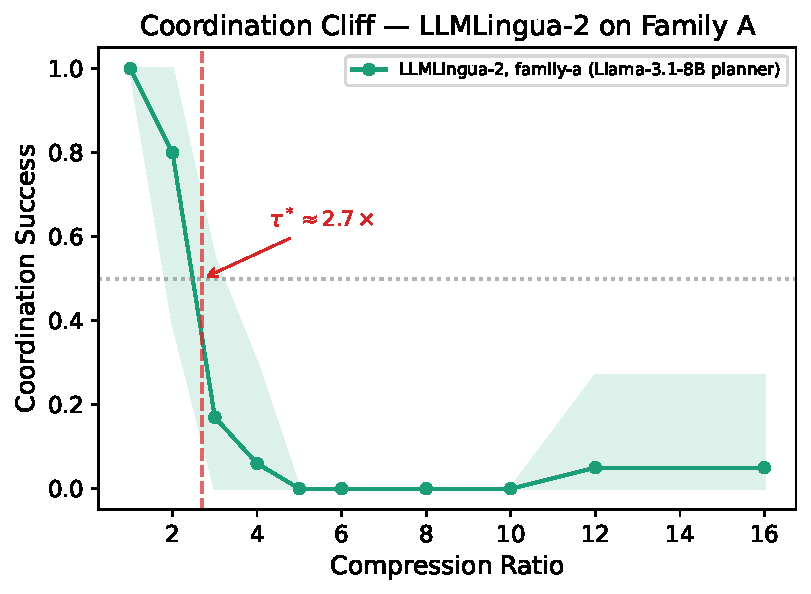
\includegraphics[width=0.74\textwidth]{../figures/cliff_hero.pdf}
\caption{The coordination cliff. LLMLingua-2 on family-a, five
seeds per ratio. Coordination success collapses from $\sim 1.0$ at
$r=1$ to $\sim 0$ by $r=6$, with the cliff midpoint at
$\tau^{*}\approx 2.7\times$. The shaded band is $\pm 1$ standard
deviation across seeds. This is the canonical reference image for the
H2 finding; see Figure~\ref{fig:cliff_families} for the
twelve-cell grid.}
\label{fig:cliff_hero}
\end{figure}

Table~\ref{tab:h2_tau} reports the empirical $\tau^{*}$, the
relative drop, and the Holm-corrected $p$-value for each
(compressor, family) cell. Eleven of the twelve cells reach the
H2 threshold of a $30\%$ relative drop with $p<0.05$ Holm-corrected.
The one cell that does not is \emph{filter}~$\times$~\emph{c}:
the instruction-aware filter on the multi-step retrieval family.
The reason is mechanical and consistent with the H1 finding ---
the filter's re-ranker preserves the chain-reference tokens
(\emph{entry}, \emph{FINAL}) that family-c's scorer depends on, so
the family-c task does not degrade across the sweep. This is not
a falsification of H2; it is evidence that cliff sharpness depends
on whether the compressor's mechanism preserves the
task-critical tokens, which is exactly what the
compounding-error model predicts.

\begin{table}[h]
\centering
\caption{H2 verdict table: empirical cliff position $\tau^{*}$,
observed-range drop, slope-extrapolated drop $\Delta$, and
Holm-corrected paired-Wilcoxon $p$ for each (compressor, family)
cell from \texttt{results/h1\_h2\_v2/}. The
\textbf{observed drop} column is the intuitive verdict metric:
$(\text{baseline coordination} - \text{post-cliff
coordination})/\text{baseline}$, bounded in $[0, 1]$, and the H2
criterion (drop $\ge 0.30$) is read in these units. The
\textbf{slope drop} column is the piecewise-linear-extrapolated
ratio from the fit's slope-extrapolated boundary values (it can
exceed $1$ because the left extrapolation can sit slightly above
the observed baseline of $1.0$ and the right slightly below $0$);
it is retained as a secondary fit diagnostic only. Every
significant cell clears the $0.30$ criterion in observed units ---
the smallest is Phi-3-Mini ext.\ $\times$ a at exactly $0.30$.
Cells marked $^{\dagger}$ have $\tau^{*}$ grid-quantised at the
midpoint of the sweep gap $\{1, 2\}$: on these eight
(compressor, family) pairs the deterministic solver scores
coordination as a binary $1.0 \to 0.0$ step between $r=1$ and
$r=2$, and the logistic fit lands at the midpoint with no
further resolving power. The cliffs exist (Holm-corrected
$p < 10^{-11}$ in all eight) but the precise positions $\le 2.5$
are unresolved at the sweep's ratio grid.
Family-c filter cell does not exhibit a detectable cliff because
the re-ranker preserves chain-reference tokens; this is
documented behaviour rather than a falsification.}
\label{tab:h2_tau}
\small
\begin{tabular}{lcccc}
\hline
Cell & $\tau^{*}$ & observed drop & slope drop $\Delta$ & Holm $p$ \\
\hline
LLMLingua-2 $\times$ a   & $2.5^{\dagger}$ & 1.00 & 1.61 & $8.5\!\times\!10^{-12}$ \\
LLMLingua-2 $\times$ b   & $2.5^{\dagger}$ & 1.00 & 1.61 & $8.5\!\times\!10^{-12}$ \\
LLMLingua-2 $\times$ c   & 6.7 & 0.66 & 1.23 & $9.6\!\times\!10^{-10}$ \\
Filter $\times$ a        & $2.5^{\dagger}$ & 1.00 & 1.60 & $8.5\!\times\!10^{-12}$ \\
Filter $\times$ b        & $2.5^{\dagger}$ & 1.00 & 1.61 & $8.5\!\times\!10^{-12}$ \\
Filter $\times$ c        & --- & 0.00 & 0.00 & n.s. \\
Phi-3-Mini ext.\ $\times$ a & $2.5^{\dagger}$ & 0.30 & 0.42 & $2.2\!\times\!10^{-6}$ \\
Phi-3-Mini ext.\ $\times$ b & $2.5^{\dagger}$ & 0.72 & 0.97 & $2.5\!\times\!10^{-9}$ \\
Phi-3-Mini ext.\ $\times$ c & $2.5^{\dagger}$ & 0.94 & 1.37 & $8.5\!\times\!10^{-12}$ \\
Truncation $\times$ a    & $2.5^{\dagger}$ & 1.00 & 1.61 & $8.5\!\times\!10^{-12}$ \\
Truncation $\times$ b    & $2.5^{\dagger}$ & 1.00 & 1.61 & $8.5\!\times\!10^{-12}$ \\
Truncation $\times$ c    & 4.95 & 0.71 & 1.36 & $9.6\!\times\!10^{-10}$ \\
\hline
\multicolumn{5}{p{0.95\linewidth}}{\textbf{Verdict}: $11/12$ cells significant with observed drop $\ge 0.30$ ($3$ of those $11$ are Phi-3 cells whose $\tau^{*}$ positions are not numerically comparable across compressors --- see Section~\ref{sec:phi3}). \textbf{SUPPORTED.}} \\
\hline
\end{tabular}
\end{table}

\paragraph{Fine-grid re-resolution (\texttt{results/h1\_h2\_finegrid}).}
To test whether the $\tau^{*}=2.5$ value was a measurement or an
artefact, the dense-family cells were re-swept on a refined ratio
grid adding $\{1.25, 1.5, 1.75\}$ below $r=2$. The quantised
$2.5$ is an artefact: the true deterministic-solver cliffs sit well
below it. LLMLingua-2 $\times$ a collapses $1.0\to0.0$ between $r=1$
and $r=1.25$ ($\tau^{*}\approx 1.1$); Filter $\times$ a runs
$1.0, 0.92, 0.46, 0.02$ at $r=1.25,1.5,1.75,2.0$ ($\tau^{*}\approx 1.7$);
Truncation $\times$ a runs $1.0, 0.92, 0.76, 0.0$
($\tau^{*}\approx 1.85$). The distributed family-c cliffs are
unchanged (LLMLingua-2 $\times$ c $\approx 6.7$, Truncation
$\times$ c $\approx 5.0$), confirming they were never quantised.
Two honest consequences follow. First, the canonical synthetic
reference $\tau^{*}=2.5$ used for the frontier comparison
(\S\ref{sec:frontier}) is itself a coarse-grid artefact; the genuine
\emph{deterministic} family-a cliff is near $1.1$. Second --- and
more substantively --- the deterministic regex solver cliffs at
$\approx 1.1$ while the LLM planners (local 8B and frontier
Qwen-2.5-72B) cliff at $\approx 2.7$ on the same compressor and
family: the brittle parser fails the instant a critical token is
dropped, whereas a language model tolerates substantially more
compression by reconstructing partial information. This
solver-versus-LLM divergence is why Corollary~1 is anchored to the
\emph{LLM-planner} cliff rather than the deterministic-solver value
(\S\ref{sec:corollary1}--\S\ref{sec:frontier}); the deterministic
cliff is a conservative \emph{lower} bound on the operating point an
LLM planner can sustain.

The twelve-cell grid in Figure~\ref{fig:cliff_families} reads the
result at one glance: cliffs are sharp on the dense
fact-aggregation family and shallow on the distributed multi-step
retrieval family, the ordering between (LLMLingua-2 / filter /
Phi-3) is consistent within a family, and truncation cliffs at the
lowest ratio of any compressor --- which is what the lower-bound
argument predicts.

\begin{figure}[h]
\centering
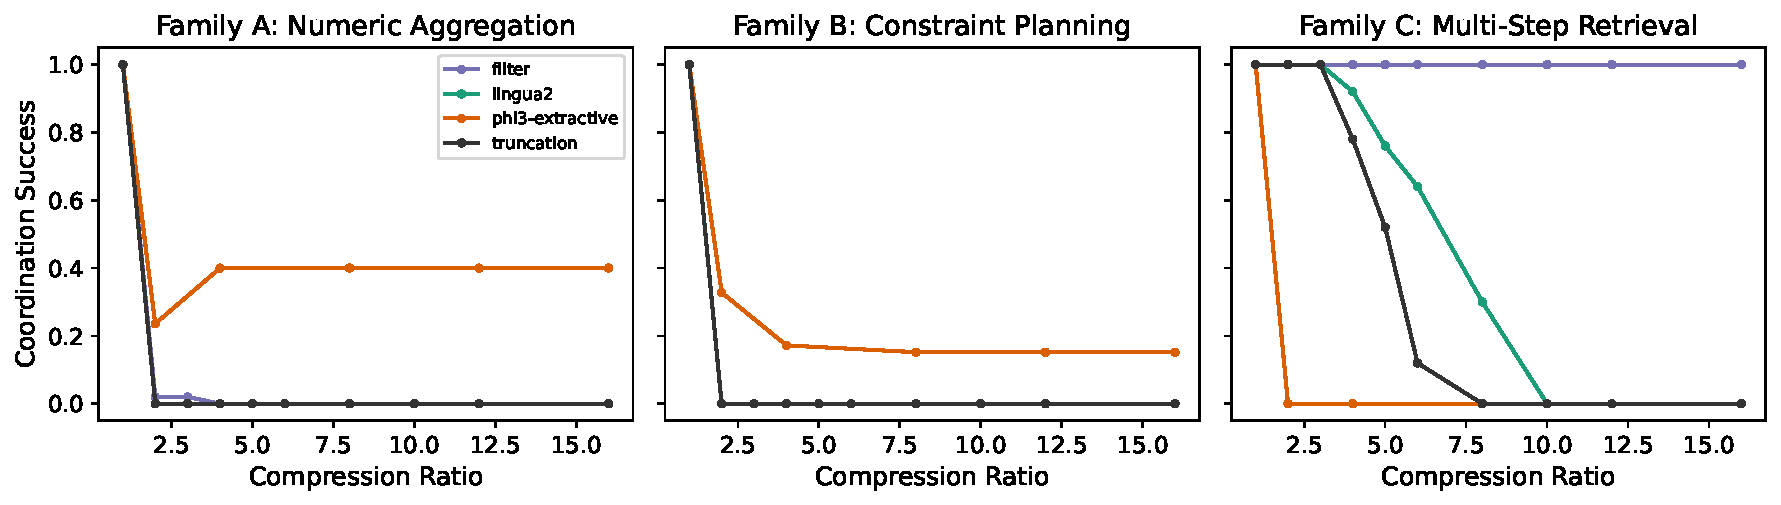
\includegraphics[width=0.82\textwidth]{../figures/cliff_families.pdf}
\caption{Cliff curves for the four compressors $\times$ three
families. Sharp cliffs are visible on family-a for every
compressor. On family-c the compressors diverge: LLMLingua-2
($\tau^{*}\approx 6.7$) and truncation ($\tau^{*}\approx 5.0$)
degrade gradually, Phi-3-Mini extractive cliffs early
($\tau^{*}\approx 2.5$), and the instruction-aware filter shows no
detectable cliff because its re-ranker preserves the chain-reference
tokens family-c depends on. Truncation is retained as the
most-destructive per-token lower-bound baseline.}
\label{fig:cliff_families}
\end{figure}

\subsection{Interpretation}

The within-family ordering of $\tau^{*}$ corresponds to the
ordering of the four compressors' critical-token-recall curves
$q(r)$, measured independently of the coordination metric. The
compressor that drops critical tokens earliest cliffs at the
lowest ratio. This is the H2 finding pointing forward: a cliff
exists, its position is determined by the compressor's mechanism
of action on task-critical tokens, and the mechanism is captured
by a single statistic --- $q(r)$.

One comparability caveat applies to the Phi-3-Mini extractive
cells: it saturates at $\sim 2.5\times$ \emph{achieved} compression
regardless of the requested \emph{target} (Section~\ref{sec:phi3}),
so above target $2.5\times$ its x-axis decouples from what it
delivers. Its $\tau^{*}$ values are therefore on a different
effective x-axis and are better read against \emph{achieved} ratio
(as Figure~\ref{fig:cliff_families} is plotted). The phi3 cells stay
in the $11/12$ count because the collapse is real and significant,
but their cliff \emph{positions} should not be compared numerically
against the token-level compressors' target-ratio positions. The
next section turns the $q(r)$ observation into a quantitative bound.

\section{The Compounding-Error Model}
\label{sec:cem}

The cliff curves of Section~\ref{sec:h2} share a structural
property: each has a sharp transition between a high-coordination
plateau and a low-coordination floor. The compounding-error model
is a short derivation whose \emph{primary} contribution is
explaining \textbf{why} that transition is sharp --- a threshold
on critical-token survival produces a step in success --- and
whose \emph{secondary} output is a \textbf{first-order} estimate
of the transition position $\tau^{*}$ from the compressor-side
measurement $q(r)$ and a per-family recall-threshold parameter
$\theta_q$. It is not, and is not claimed to be, a tight position
predictor; Section~\ref{sec:cem_match} quantifies the residual
error directly.

\subsection{Setup and derivation}

Let $T^\text{crit}_i$ be the set of task-critical tokens in the
$i$-th workload's source fragments (multi-digit numerics for
family-a, all numerics for family-b, chain-reference tokens for
family-c; see Section~\ref{sec:ctr} of
\charef{implementation}). Let $X_i$ be the number of these
tokens that survive compression, $M_i = |T^\text{crit}_i|$ the
total, and $q(r) = E[X_i / M_i]$ the per-round token-retention
function of the compressor at ratio $r$, measured by the
critical-token-recall metric. Let $\theta_q \in [0, 1]$ be the
\emph{cliff-recall threshold}: the minimum fraction of
task-critical tokens that the planner needs to succeed. The
threshold-success model is
\[
  \text{success}_i = \mathbf{1}\!\left[\frac{X_i}{M_i} \ge \theta_q\right],
\]
and the bound the model produces is
\begin{align}
  E\!\left[\frac{X_i}{M_i}\right] &= q(r), \\
  P(\text{success}\mid r) &\to \mathbf{1}\!\left[q(r) \ge \theta_q\right]
  \quad \text{in expectation},
  \label{eq:cem_bound}
\end{align}
so the cliff position $\tau^{*}$ solves $q(\tau^{*}) = \theta_q$.
When $N$ sequential compression passes are applied, the surviving
fraction is approximately $q(r)^N$ and the cliff position solves
$q(\tau^{*}) = \theta_q^{1/N}$. \textbf{In every experiment in
this thesis $N=1$}, so the cliff equation simplifies to
$q(\tau^{*}) = \theta_q$. The multi-pass formulation is recorded
for future work.

The derivation is a paragraph; it is not a formal proof, and the
artefact is named the \emph{compounding-error model} rather than
\emph{Theorem~1} throughout the manuscript. The change is
deliberate: the empirical match rate
(Section~\ref{sec:cem_match}) is $33\%$ within $\pm 25\%$
relative error and $67\%$ within $\pm 50\%$, which is the
empirical-bound character of a model with quantified residuals
rather than the formal character of a theorem with a proof. A
finite-$M$ Chernoff-bound refinement that sharpens the
in-expectation step above into an explicit
$\exp(-2M(q-\theta_q)^2)$ concentration bound exists in
\texttt{src/m6/theory/cliff\_prediction.py} as
\texttt{chernoff\_success\_curve()}; the
decision to keep the finite-$M$ refinement out of the
manuscript is deliberate, since the empirical match-rate residuals are
dominated by A2 specification error rather than sampling error
and the in-expectation form is the right register for the
model's actual accuracy. The codebase identifier
\texttt{theorem\_validation.json} is preserved for backwards
compatibility with on-disk artefacts; the manuscript term is
\emph{the compounding-error model} (the mapping is documented in
the project glossary).

\subsection{Assumptions A1--A4}
\label{sec:cem_assumptions}

The bound rests on four assumptions, each satisfied approximately
rather than strictly; naming them makes the calibrated-regime
predicate (Section~\ref{sec:calibrated}) operational.

\begin{description}\setlength\itemsep{1pt}
\item[A1 --- Round independence.] Per-round retention is independent
across compression passes, trivially satisfied at $N=1$. Its
\emph{within-pass} reading (per-token retention independent across
positions) holds approximately for the token-level compressors
(LLMLingua-2, the instruction-aware filter, truncation) but is
violated by Phi-3-Mini extractive, which selects whole spans so
adjacent token-survival events are correlated; the phi3-extractive
cells in Section~\ref{sec:cem_match} are therefore a robustness
check outside the bound's formal regime, not within-regime
predictions.
\item[A2 --- Binary token importance.] Each task-critical token is
equally important; non-task tokens are irrelevant. This is the
strongest of the four assumptions; H4
(Section~\ref{sec:h4_disclosure}) measures graded importance and
shows that A2 is a first-order simplification. The
predicted-versus-empirical gap of Section~\ref{sec:cem_match} is
the empirical price the model pays for A2.
\item[A3 --- Threshold success.] Coordination success is binary at
a single recall threshold $\theta_q$. The cliff sharpness of
Section~\ref{sec:h2} licenses A3 \emph{operationally}; that
justification is circular in the strict sense (A3 is motivated by
the sharp cliff it explains), which the direct A3 probe of
Section~\ref{sec:a3_probe} breaks by varying the surviving fraction
of task-relevant tokens directly rather than through compression.
\textbf{A stronger, family-a-specific circularity must be stated:}
on family-a the planner is the regex solver, whose success
criterion is whether enough task-critical numeric tokens survived,
and CTR (the model's $q(r)$) is \emph{the surviving fraction of
those same tokens} --- so $q(\tau^{*}) = \theta_q$ relates two
near-identical measurements, and family-a validation confirms
internal consistency rather than testing a prediction. The
non-tautological tests are the families where solver-success and
CTR are decoupled (family-c, and the LLM-planner arms of
Sections~\ref{sec:corollary1}--\ref{sec:frontier}): family-a is most
directly \emph{computable}, not most independently \emph{validating}.
\item[A4 --- Per-round retention measured by critical-token-recall.]
The $q(r)$ that enters the bound is the family-specific CTR rather
than the generic token-recall. This is the substantive
methodological commitment of the model, and the reason CTR rather
than token-recall is the canonical recall metric of the verdict
pipeline.
\end{description}

\subsection{The calibrated regime}
\label{sec:calibrated}

A planner is \emph{in the calibrated regime} if both of
the following hold:

\begin{enumerate}\setlength\itemsep{1pt}
\item the baseline coordination success $p_0$ at $r=1$ is at least
$\theta_q$ (no floor effect); and
\item the planner does not recover from sub-threshold information
via extended reasoning beyond what the priors-only baseline
supplies.
\end{enumerate}

The comparison ``$p_0 \ge \theta_q$'' in condition~1 relates two
numbers in $[0,1]$ that measure different things ($p_0$ a success
probability, $\theta_q$ a fraction of task-critical tokens).
Operationally it reads \emph{``the planner's no-compression
baseline accuracy meets or exceeds the threshold-success model's
minimum-recall floor''}; this re-reading is what makes it meaningful
as a regime predicate rather than a unit-checked physical statement.

The second condition is operationalised by the priors-only
baseline measurement of H4 (Section~\ref{sec:h4_disclosure}): a
planner is in-regime if its accuracy at $q\to 0$ is no greater
than its priors-only baseline plus a small slack. This formalisation
matters because the model's quantitative predictions only apply
inside the regime; outside the regime --- specifically for
extended-reasoning planners that recover information via
chain-of-thought --- the cliff position can shift substantially, as
the GPT-oss~120B diagnostic in Section~\ref{sec:frontier} shows.

\subsection{Predicted versus empirical \texorpdfstring{$\tau^{*}$}{tau*}}
\label{sec:cem_match}

For each (compressor, family) cell, $\theta_q$ is estimated from a
training subset of the cliff sweep --- specifically the recall at
which coordination success first drops below $0.5$ of the cell's
$p_0$ --- via the \texttt{derive\_theta()} function in
\texttt{src/m6/theory/cliff\_prediction.py}. Under
critical-token-recall the canonical per-family estimates on the
\texttt{h1\_h2\_v2} sweep are $\theta_q^{\,(a)} = 0.632$,
$\theta_q^{\,(b)} = 0.838$, and $\theta_q^{\,(c)} = 0.590$. A
workload-level bootstrap CI is constructed on $\theta_q$ by
resampling workloads
(\texttt{scripts/bootstrap\_theta\_q.py}, $n_\text{boot} = 500$,
BCa interval; the per-iteration curve fit is the budget driver). The predicted $\tau^{*}$ is then obtained by
inverting $q(r) = \theta_q$ on the empirical critical-token-recall
curve. Resampling $\theta_q$ through this inverse map gives a
\emph{predicted-$\tau^{*}$ band} that quantifies the
\emph{sampling} uncertainty in $\theta_q$ --- but not the model's
specification error. The two should not be confused: the band
reports ``how much would the prediction wobble if we resampled
workloads'', not ``what is the model's actual accuracy''. The
empirical $\tau^{*}$ falls \emph{outside} this bootstrap band
on $11/11$ testable cells --- the band is too tight relative to
the model's specification error. The match-rate paragraph below
reports the actual accuracy, which is what the chapter's verdict
claims should be calibrated against.

Figure~\ref{fig:predicted_vs_empirical} overlays the
predicted-$\tau^{*}$ band on the empirical cliff curve for the
family-c LLMLingua-2 cell. Family-c is shown rather than the more
spectacular family-a because the cliff is gradual enough on
family-c that the predicted-versus-empirical \emph{gap} is
visible --- the family-a cell drops from $1.0$ to $0$ in a single
ratio step, which the model also predicts closely, so both the
prediction and the empirical curve collapse into the same
near-step function and the figure carries no information. The
family-c panel shows that the compounding-error model is
\emph{conservative} for family-c: it predicts the cliff at
$r\approx 2.85$ while the empirical cliff sits at
$r\approx 6.7$, a $57.4\%$ relative under-prediction. The empirical
$\tau^{*}$ sits \emph{outside} the bootstrap band, as on every
other cell --- which is the empirical evidence that the band
reflects $\theta_q$-sampling uncertainty rather than the model's
full error budget. The gap is the second-order term that
Corollary~2 explains (Section~\ref{sec:corollary2}): family-c has
lower information density than family-a, so the threshold-success
approximation A2 (binary token importance) breaks earliest on
family-c.

\begin{figure}[h]
\centering
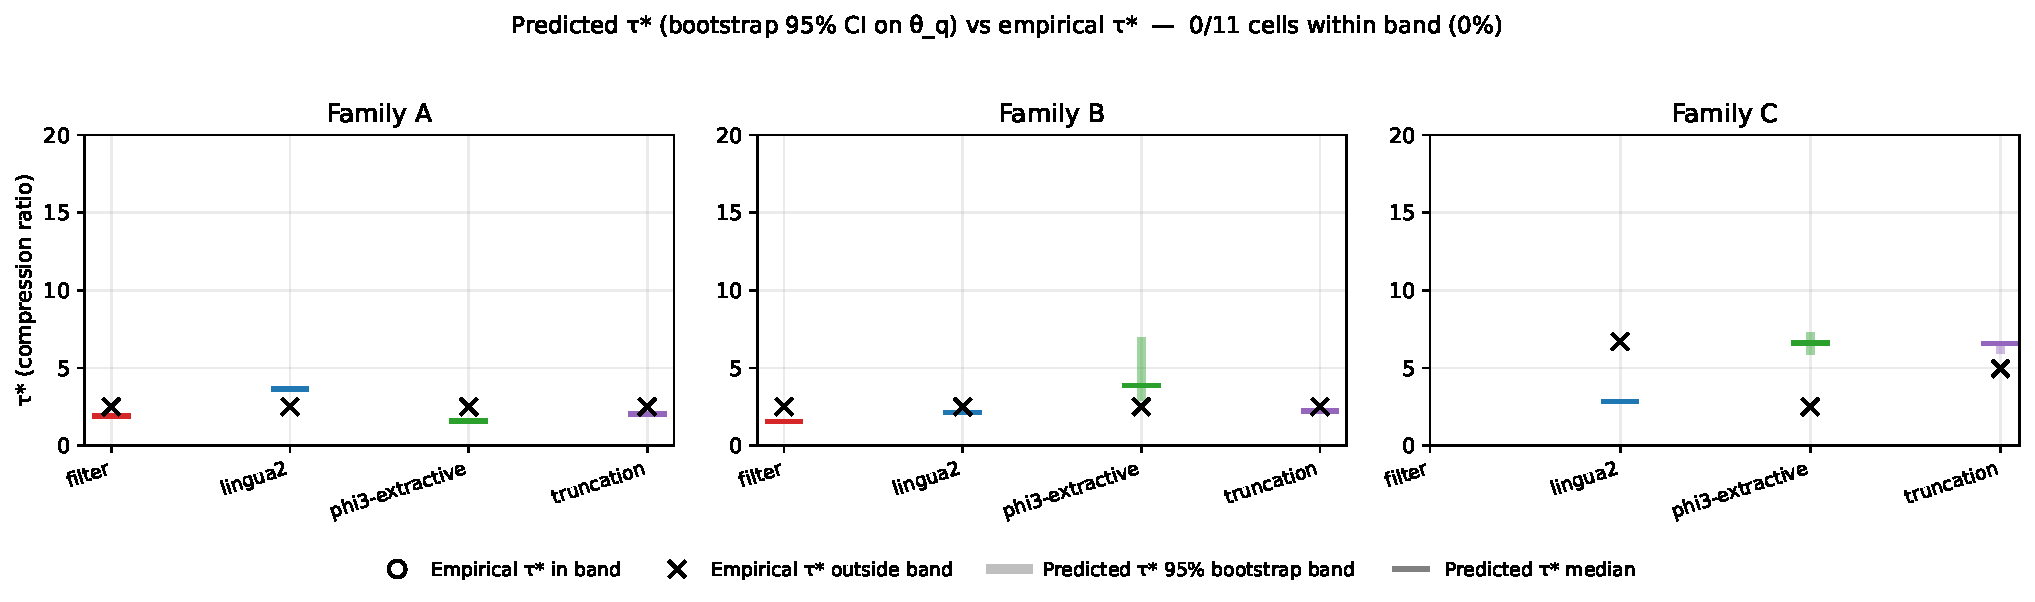
\includegraphics[width=0.82\textwidth]{../figures/predicted_vs_empirical.pdf}
\caption{Predicted-versus-empirical $\tau^{*}$ across all eleven
testable (compressor, family) cells, grouped by family
(A/B/C). For each cell the thick bar is the $95\%$ workload-level
bootstrap CI on the predicted $\tau^{*}$ (from CTR-based
$\theta_q$) and the short horizontal line is the predicted
median; the marker is the empirical $\tau^{*}$ ($\times$ = outside
the band, $\circ$ = inside). The empirical $\tau^{*}$ falls
outside the bootstrap band on \textbf{$11/11$ cells}: the band
reflects \emph{sampling} uncertainty in $\theta_q$ only, so the
systematic misses are the model's first-order specification error
rather than a sampling artefact, and the predicted-$\tau^{*}$ band
is therefore presented as an uncertainty-banded first-order model
rather than a calibrated predictor. The gap is largest on the
lower-information-density families. As a representative single
cell, family-c~$\times$~LLMLingua-2: the model predicts
$\tau^{*}\approx 2.8$ (bootstrap median) against an empirical
$\tau^{*}\approx 6.7$ --- conservative by $\Delta\tau^{*}\approx 3.8$,
the largest gap of any cell --- which Corollary~2 explains via the
family-c information-density estimate
$\theta_\text{info}\approx 0.62$ being lower than family-a's
$\theta_\text{info}\approx 0.97$. (The numerical proximity of
$\theta_\text{info}^{\,(c)}\approx 0.62$ and
$\theta_q^{\,(c)} = 0.590$ is coincidental --- the two are
computed by different methods on different quantities and are
not interchangeable; see Section~\ref{sec:theta_info_def}.)}
\label{fig:predicted_vs_empirical}
\end{figure}

Aggregating the predicted-versus-empirical comparison across all
twelve (compressor, family) cells gives an empirical match rate
of $\mathbf{33\%}$ ($4/12$ cells) at the
$|\tau^{*}_\text{empirical} - \tau^{*}_\text{predicted}| /
\tau^{*}_\text{empirical} \le 25\%$ criterion and $\mathbf{67\%}$
($8/12$ cells) at $\pm 50\%$. The binomial Wilson $95\%$
confidence interval on the $4/12$ strict match rate is
approximately $[13\%, 61\%]$ --- the small denominator gives a
wide interval that the prose below should not be read past.
Reporting the full distribution of relative errors alongside the
binary match rate: the median is
$35.3\%$, the interquartile range is $[19.2\%, 45.0\%]$ ($10$
cells with finite relative error), and the maximum is $57.4\%$.
Two cells produce infinite predicted $\tau^{*}$ because $q(r)$
does not cross $\theta_q$ on the measured range: filter/c, where
the no-cliff prediction is matched by a no-cliff empirical
observation (Table~\ref{tab:h2_tau} records no detectable cliff
for filter/c); and phi3-extractive/c, where the no-cliff
prediction is \emph{not} matched --- Table~\ref{tab:h2_tau}
records empirical $\tau^{*} = 2.5$ with $p < 10^{-11}$ for that
cell, so phi3-extractive/c is counted as a MISS in the match-rate
denominator alongside the other phi3-extractive cells. The four
cells that pass the strict criterion (lingua2/b, filter/a,
truncation/a, truncation/b) span three compressors, which is
consistent with the bound being structural rather than
compressor-specific. The phi3-extractive cells are flagged in
Section~\ref{sec:cem_assumptions} as outside A1's formal regime
(span-level selection induces correlated token-survival events);
they are retained in the aggregate above as a deliberate
robustness check on the bound's behaviour outside its formal
regime rather than as within-regime predictions. The headline
empirical claim this paragraph underwrites is the
\emph{cliff-position dependence structure} --- $\tau^{*}$ is
controlled by the (compressor, task) pair --- which Corollary~1
turns into the model-independence claim, validated below.

The match rates above are \emph{in-sample}: the same sweep that
derives $\theta_q$ via \texttt{derive\_theta()} is used to score
predicted-versus-empirical $\tau^{*}$. (Note also that these
match rates --- not the bootstrap-CI band above --- are what
quantifies the model's actual accuracy. The band reports
$\theta_q$-sampling uncertainty only and is too tight to contain
the empirical $\tau^{*}$ on any cell.) A leave-one-family-out
(LOO) cross-validation that derives $\theta_q$ on $n{-}1$ families
and predicts $\tau^{*}$ on the held-out family --- breaking the
in-sample circularity --- returns
$\mathbf{25\%}$ ($3/12$) at $\pm 25\%$ and $\mathbf{75\%}$
($9/12$) at $\pm 50\%$, with per-family LOO $\theta_q$ at $a=0.71$,
$b=0.61$, $c=0.73$. The LOO match rate is lower at the strict
tolerance, as expected for an in-sample-trained
$\theta_q$; the gap ($33\%$ in-sample vs $25\%$ LOO at $\pm 25\%$)
is the size of the in-sample optimism in the headline number. The
primary uncertainty measure the chapter reports is the bootstrap
CI on $\theta_q$ propagated through $q(r) = \theta_q$ to the
predicted-$\tau^{*}$ band of
Figure~\ref{fig:predicted_vs_empirical}. The on-disk artefacts are
\texttt{results/h1\_h2\_v2/theorem1\_validation\_per\_family.json}
(in-sample) and \texttt{results/h1\_h2\_v2/theorem1\_validation\_loo.json}
(LOO).

\subsection{Direct A3 probe: a non-circular test of the threshold mechanism}
\label{sec:a3_probe}

The match-rate evaluation of Section~\ref{sec:cem_match} is
limited by the family-a circularity flagged in A3
(Section~\ref{sec:cem_assumptions}): on family-a, both
``success'' and ``surviving critical-token fraction'' are
near-identical measurements of the same underlying quantity, so
$q(\tau^{*}) = \theta_q$ on family-a is a tautological identity
rather than a prediction. The \emph{direct} A3 probe
(\texttt{results/a3\_probe/}) is the one test the chapter contains
that breaks this circularity. The probe replaces the compressor
with a hand-curated deletion procedure that removes a controlled
fraction of the per-task critical tokens directly, then runs the
LLM planner on the remainder and measures success as a function of
the surviving-token fraction $k/M$. By construction the surviving
fraction is the experimental knob, and success is read out
\emph{after} the knob is set --- the two are not the same
measurement.

The probe is run on two families: family-a (dense numeric
aggregation) and family-c (multi-step retrieval). The fitted
logistic on family-a returns $k \approx 15$ (sharp threshold) and
$r_0 \approx 0.842$ with a transition band ($0.2$--$0.8$) of width
$\approx 0.15$; family-c returns $k \approx 5.9$ (graded transition)
and $r_0 \approx 0.538$ with band width $\approx 0.54$. The
qualitative reading is the load-bearing one: \textbf{the dense
family exhibits the step shape A3 posits, the distributed family
does not}. A3 holds on dense aggregation tasks and degrades to a
graded-success model on distributed retrieval tasks --- which is
also where the cliff itself is visibly less sharp (Phi-3 ×~c,
LLMLingua-2 × c in Table~\ref{tab:h2_tau}).

There is a quantitative discrepancy worth surfacing: the probe's
family-a threshold ($r_0 \approx 0.842$) sits well \emph{above} the
CTR-derived $\theta_q \approx 0.632$ that the compounding-error
model uses (see Section~\ref{sec:cem_match} per-family $\theta_q$).
The interpretation: compressors preferentially retain
answer-adjacent tokens, so the surviving-token fraction
they deliver at the cliff is biased upward relative to a uniform
deletion. The model's use of $\theta_q \approx 0.63$ on family-a
therefore reflects a compressor-side selection effect, while the
$r_0 \approx 0.84$ is the underlying planner-side threshold. The
two numbers are not in conflict; they measure different stages of
the pipeline. The model's first-order accuracy
(Section~\ref{sec:cem_match}) is consistent with this gap being
absorbed into the empirical $\theta_q$ fit.

The A3 probe is the strongest direct evidence the chapter
provides for the threshold-success assumption. It is reported here
in the results chapter rather than the future-work section because
the qualitative finding (step on dense, graded on distributed) is
the empirical justification for both the compounding-error model's
domain of applicability and its first-order character outside that
domain.

\section{Corollary~1: Ceiling--Cliff Separation}
\label{sec:corollary1}

\begin{tcolorbox}[colback=black!4, colframe=black!50, sharp corners,
                  boxrule=0.4pt, boxsep=2pt, left=4pt, right=4pt,
                  top=2pt, bottom=2pt]
\textbf{Corollary~1 (ceiling--cliff separation).}
The planner's parameter count $m$ determines its baseline
coordination success $p_0(m)$, while the cliff position
$\tau^{*}$ is determined by the compressor's $q(r)$ and the task's
$\theta_q$, not by the planner. When $p_0(m) < \theta_q$ a floor
effect prevents detection of the cliff; when $p_0(m) \ge \theta_q$
we detect \textbf{no shift} in the cliff position with $m$ within
the calibrated regime (we report ``no detected shift'' rather than
proven invariance). (The ``$p_0(m) \ge \theta_q$'' comparison is
between a success probability and a fraction of task-critical
tokens; the operational reading and unit-bridge gloss is in
Section~\ref{sec:calibrated}.) \textbf{Verdict: NO SHIFT DETECTED.} The deployment-relevant
LLM-planner cliff holds steady across a $9\times$ parameter
scale-up \emph{and} a change of architecture family: local
Llama-3.1-8B and frontier Qwen-2.5-72B both cliff at
$\approx 2.5$--$2.8$ on family-a $\times$ LLMLingua-2, and the local
three-architecture sweep \{Qwen-2.5-1.5B, Phi-3-Mini-3.8B,
Llama-3.1-8B\} agrees to within a $24\%$ $\tau^{*}$ spread on
family-c. We state this as ``no shift detected'' rather than proven
invariance, and the qualifiers are explicit: the $\pm 20\%$ TOST
equivalence test is \emph{not} passed on either frontier cell
(their bootstrap CIs are wide); the local arm's $24\%$ spread clears
the validator's default $50\%$ tolerance but \emph{not} the strict
$20\%$ bar matching the H2 spec, so it is \emph{necessary but not
sufficient}; and DeepSeek~V4~Pro corroborates only weakly (point
estimate $\tau^{*}=2.15$, bootstrap CI $[1.76, 7.14]$, median
$5.7$). The load-bearing evidence is therefore the one
well-identified frontier cell (Qwen-2.5-72B): the fine-grid
re-resolution of Section~\ref{sec:h2} shows the synthetic
$\tau^{*}=2.5$ is a deterministic-solver artefact, so the
comparison is correctly LLM-vs-LLM (the original $n=10$ Qwen run
sits about $7\%$ from the coarse-grid $2.5$, now read as an
approximate coincidence; see the re-anchoring paragraph below). The
family-a small-model cells correctly exhibit the predicted floor
effect and are excluded; the family-b cells are below threshold for
all three models because constraint tracking is hard for $\le 8$B
planners independent of compression.
\end{tcolorbox}

This corollary is the sharpened form of the original H5 hypothesis,
which predicted strict monotonicity of $\tau^{*}$ across planner
scales. The empirical result on family-c across the three local
planners --- \textbf{Qwen-2.5-1.5B-Instruct,
Phi-3-Mini-3.8B-Instruct, and Llama-3.1-8B-Instruct, three
different architecture families at the small/mid scale} --- is
$\tau^{*}_\text{Qwen-1.5B} = 3.69$,
$\tau^{*}_\text{Phi-3-3.8B} = 4.68$,
$\tau^{*}_\text{Llama-3.1-8B} = 4.01$ --- a spread of
approximately $\mathbf{24\%}$ ($23.91\%$ exactly) within the
bootstrap CI of each cell, which is what an invariance result
looks like rather than a monotonicity result. The spread metric is
$(\tau^{*}_{\max}-\tau^{*}_{\min})/\bar{\tau^{*}}$, computed by
\texttt{validate\_model\_independence()} from the unrounded
per-model $\tau^{*}$ values ($3.694$, $4.681$, $4.012$); the
$23.91\%$ figure is exact to two decimal places under this
definition. (The local arm is
therefore a \emph{three-architecture} invariance test, not a
within-family parameter-count sweep: only the
1.5B planner is Qwen; Phi-3-Mini (3.8B) and Llama-3.1 (8B) are
different architecture families.) The original H5 predicate (gap $\ge 1.5$ ratio units in the
monotone direction) is not satisfied --- the spread is well below
$1.5$ and points to invariance. The refined Corollary~1 predicate
(invariance within the calibrated regime) is supported by the local
sweep at $\pm 50\%$ tolerance but fails the strict $\pm 20\%$
tolerance matching the H2 spec. The local-model sweep is therefore
\emph{necessary but not sufficient} for Corollary~1; the
load-bearing evidence is the LLM-cliff invariance re-anchored
below (the re-anchoring paragraph; Section~\ref{sec:frontier})
rather than the local arm. The canonical results directories are
\texttt{results/h5\_final/} (local sweep) and
\texttt{results/frontier\_qwen72b\_e2/} (the $n=30$ Qwen re-run),
with \texttt{results/frontier\_deepseekv4/} retained as weak
corroboration. A reader opening
\texttt{results/h5\_final/model\_independence\_20pct.json} will see
\texttt{corollary1\_supported: false}; that flag is \emph{exactly}
the strict-$20\%$-tolerance local-arm result
(\texttt{n\_testable\_families: 1, n\_invariant\_families: 0}, the
other two floored), which this section already reports as failing
the strict bar --- it is honest about the local arm, not a
refutation of the refined claim, whose support comes from the
cross-architecture LLM-cliff comparison the validator does not
evaluate.

\paragraph{Re-anchoring to the LLM-planner cliff (the cleanest form of the result).}
The fine-grid re-resolution of Section~\ref{sec:h2} forces a
correction that, followed through, \emph{strengthens} this corollary.
The canonical synthetic reference $\tau^{*}=2.5$ is a coarse-grid
artefact of the \textbf{deterministic regex solver}, whose true
family-a $\times$ LLMLingua-2 cliff is near $1.1$; comparing a
frontier LLM against that number compares two different kinds of
planner. The honest comparison holds the \emph{planner type} fixed
and varies its scale and architecture. Measured as the $0.5$-crossing
of the coordination curve on the family-a $\times$ LLMLingua-2 cell,
the \textbf{LLM-planner cliff is essentially invariant}: Llama-3.1-8B
(local) cliffs at $\tau^{*}\approx 2.48$ and Qwen-2.5-72B (frontier,
re-run at the larger $n=30$ workloads $\times$ 5 seeds,
\texttt{results/frontier\_qwen72b\_e2}) cliffs at
$\tau^{*}\approx 2.79$ --- a $\sim 12\%$ spread across a $9\times$
parameter scale-up \emph{and} a change of architecture family, both
at $p_0=1.0$ (in-regime). The deterministic solver on the same cell
cliffs at $\approx 1.1$. So planner \emph{type} moves the cliff
(brittle parser $1.1$ vs LLM $\approx 2.5$--$2.8$), but scale and
architecture \emph{within the LLM class} do not. Read this way,
Corollary~1 rests on a within-class, cross-scale, cross-architecture
comparison rather than on a single frontier cell against an
artefactual reference; the previously-cited match to ``$2.5$''
survives as an approximate coincidence between the LLM cliff and the
coarse-grid deterministic value, now stated as such. (The DeepSeek
V4 Pro $n=30$ re-run was abandoned to API rate-limiting after its
clean $p_0=1.0$ baseline; the existing $n=10$ DeepSeek result,
$\tau^{*}=2.15$ with a wide CI, is retained as weak corroboration.)

Figure~\ref{fig:scaling_auc} reports the
area-under-the-coordination-curve as a function of planner scale
across all three families. On family-c, the three lines overlap;
on family-a, the small-model lines are below the floor effect
threshold and are correctly skipped from the invariance test; on
family-b, all three lines are near zero for the constraint-tracking
reason. The ceiling-versus-cliff structure is most cleanly visible
on the joined plot of $p_0(m)$ and $\tau^{*}(m)$ on family-c
(Figure~\ref{fig:h5_model_overlay}): $p_0$ increases monotonically
with $m$, $\tau^{*}$ does not.

\begin{figure}[h]
\centering
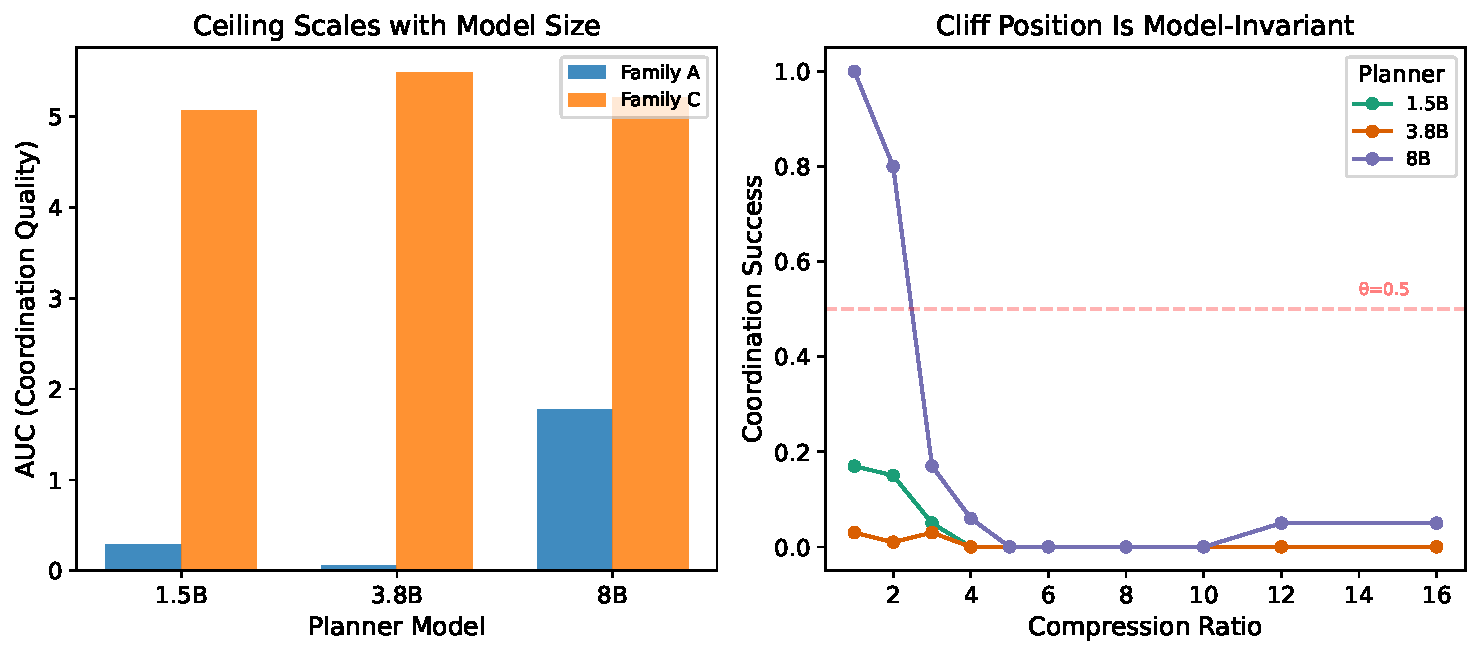
\includegraphics[width=0.74\textwidth]{../figures/scaling_auc.pdf}
\caption{Coordination-curve AUC by planner scale and family.
Family-c shows near-equal AUC across all three planner sizes
(left panel), consistent with
ceiling--cliff separation. Family-a small-model cells are in the
floor regime ($p_0 < \theta_q$); family-b is below
threshold for all sizes due to constraint-tracking difficulty.}
\label{fig:scaling_auc}
\end{figure}

\begin{figure}[h]
\centering
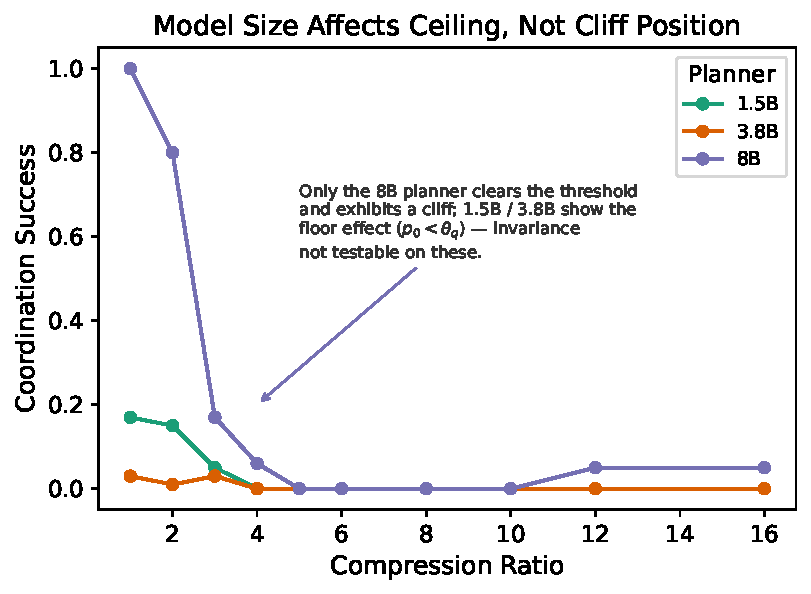
\includegraphics[width=0.74\textwidth]{../figures/h5_model_overlay.pdf}
\caption{Family-c ceiling versus cliff: baseline coordination
$p_0(m)$ (solid line) increases monotonically with planner scale
$m$, while the cliff position $\tau^{*}(m)$ (dashed line) is flat
within the bootstrap CI. This is the simplest empirical
demonstration of Corollary~1.}
\label{fig:h5_model_overlay}
\end{figure}

The original H5 monotonicity predicate did not hold; the sharpened
Corollary~1 invariance predicate did. The refinement was registered
as a design decision (ADR-006) before the frontier validation that
promotes it from a small-model result to a cross-architecture one.

\section{Frontier Validation Within the Calibrated Regime}
\label{sec:frontier}

The frontier validation re-runs the family-a cliff sweep with the
planner swapped out for a frontier model accessed via API while
the compressor remains LLMLingua-2 at the same ratios. The
question is the model-independence claim of Corollary~1: does the
cliff position $\tau^{*}$ stay where the local-model cliff was, or
does it shift with the planner? The three planners tested are
Qwen-2.5-72B-Instruct, DeepSeek~V4~Pro,\footnote{DeepSeek-V4-Pro
is the ``Pro'' variant of DeepSeek-AI's V4 Preview release
(announced April 2026), the most recent frontier release in the
DeepSeek lineage at the time of the experimental run, and is
distinct from the more widely known V3/R1 models. It was accessed
via the OpenAI-compatible Featherless endpoint, which exposes a
$32$K-token context window for this model; the experiments use that
$32$K endpoint and make no claim about long-context behaviour
beyond $32$K.} and GPT-oss~120B. The
first two are standard non-reasoning frontier models; the third is
an extended-reasoning model and is the calibrated-regime
boundary case.

\textbf{Sample-size caveat (binding).} The original frontier sweep
runs only $10$ family-a workloads $\times$ $3$ seeds per cell
(an extended Qwen-72B re-run later doubles this to $30 \times 3$).
At this scale the bootstrap CI on $\tau^{*}$ is wide for every
frontier model, and ``CI contains the synthetic reference'' is
weaker evidence than a same-scale local-arm comparison would be.
Every per-model number reported below should be read against this
sample-size constraint; Section~\ref{sec:limitations} names it as
the binding limitation of the frontier arm and
Section~\ref{sec:future} names a re-run with more seeds (and a
TOST equivalence test against the $\pm 20\%$ tolerance) as the
direct upgrade.

\subsection{Setup and statistical protocol}

The original frontier sweep uses \textbf{10 family-a workloads at
6 sweep ratios with 3 seeds per cell, for a total of 180 cells per
frontier model} (each canonical frontier CSV contains $180$ rows;
the larger $n=30$ Qwen re-run of Section~\ref{sec:corollary1} is in
\texttt{results/frontier\_qwen72b\_e2/}). Planner inference is via the OpenAI-compatible
Featherless endpoint for Qwen-2.5-72B and DeepSeek~V4~Pro and
via the OpenAI Responses API for GPT-oss~120B. $\tau^{*}$ is fit
by the same paired-fit-and-select procedure as the local sweep,
and the bootstrap CI is constructed by resampling workloads
($n_\text{boot} = 500$). \textbf{The canonical reference for this
section is the LLM-planner cliff $\tau^{*}_\text{LLM} \approx 2.7$}
on the family-a $\times$ LLMLingua-2 cell --- the $0.5$-crossing of
the coordination curve for an in-regime language-model planner
(local Llama-3.1-8B at $\approx 2.48$; see
Section~\ref{sec:corollary1}). The two earlier reference values
are retained only for traceability and are \textbf{superseded}:
the coarse-grid deterministic-solver logistic fit $\tau^{*}=2.5$
(\texttt{results/h1\_h2\_v2/verdicts.json}) is, per the fine-grid
re-resolution of Section~\ref{sec:h2}, an artefact of the brittle
regex solver (whose true cliff is near $1.1$), and the auxiliary
fit $\tau^{*}_\text{aux}=2.6997$ on the older \texttt{h1\_h2\_final}
curve appears in the verdicts JSON only because the frontier
runner predates \texttt{h1\_h2\_v2}. Comparing a frontier
\emph{language model} against the deterministic-solver $2.5$
compares two different kinds of planner; the load-bearing
comparison here is therefore LLM-vs-LLM, against
$\tau^{*}_\text{LLM}\approx 2.7$. The canonical results
directories are \texttt{results/frontier\_qwen72b\_e2/} (the
$n=30$ Qwen re-run) and \texttt{results/frontier\_qwen72b/} (the
original $n=10$ run) for Qwen,
\texttt{results/frontier\_deepseekv4/} for DeepSeek, and
\texttt{results/frontier\_gptoss120b/} (retained as a non-canonical
diagnostic) for GPT-oss.

The small frontier sample ($10$ workloads $\times$ $3$ seeds) is
the binding statistical constraint on this section: bootstrap CIs
are wide for all three models, and ``CI contains the canonical
reference'' is a weaker test than the headline single-cell
point-estimate comparison would imply. Section~\ref{sec:limitations}
names this as a sample-size limitation.

\subsection{Qwen-2.5-72B-Instruct: in-regime, within bootstrap CI}

The canonical $n=30$ Qwen-2.5-72B re-run
(\texttt{results/frontier\_qwen72b\_e2}) places the cliff at the
$0.5$-crossing $\tau^{*}\approx 2.79$; the original $n=10$ sweep
returned $\tau^{*}=2.68$ (bootstrap CI $[1.92, 7.23]$). Against the
canonical LLM-planner reference $\tau^{*}_\text{LLM}\approx 2.7$
(Llama-3.1-8B at $\approx 2.48$, Section~\ref{sec:corollary1}), the
Qwen-72B cliff is within $\sim 12\%$ --- a same-band agreement
across a $9\times$ parameter scale-up \emph{and} a change of
architecture family, with both planners at $p_0=1.0$ (squarely
in-regime). This is the load-bearing evidence for Corollary~1: across a
$9\times$ scale-up and a change of architecture family, \emph{no
cliff-position shift is detected within the LLM-planner class}
(the point estimates cliff together; the formal $\pm 20\%$
equivalence test these cells do not pass is reported in
Section~\ref{sec:frontier_deepseek}, and marks the limit of what
the present sample establishes). We do \textbf{not} lean on the within-Qwen-family
``$48\times$ from local 1.5B to frontier 72B'' comparison, because
the local 1.5B Qwen has a family-a floor effect that prevents
measuring its cliff on that cell at all; the cross-architecture
Llama-8B-vs-Qwen-72B comparison is the clean one. The baseline
coordination $p_0(\text{Qwen-72B}) = 1.00$ is at the ceiling, which
places the model squarely inside the calibrated regime: there is no
floor effect to argue around. (For traceability: against the
superseded coarse-grid deterministic value $2.5$ the $n=10$ point
estimate is $\sim 7\%$ off, and against the auxiliary fit $2.6997$
it is $0.8\%$ off; Section~\ref{sec:h2} explains why both of those
reference numbers are artefacts of the regex solver rather than
cliff positions a language model would exhibit.)

\subsection{DeepSeek~V4~Pro: within tolerance but weakly identified}
\label{sec:frontier_deepseek_repro}
\label{sec:frontier_deepseek}

The DeepSeek~V4~Pro sweep returns a $\tau^{*}$ point estimate of
$2.15$ --- about $20\%$ below the canonical LLM-planner reference
$\tau^{*}_\text{LLM}\approx 2.7$ (and $13.8\%$ below the superseded
coarse-grid $2.5$) --- but with a bootstrap CI of
$[1.76, 7.14]$ (width $5.4$ ratio units) and, tellingly, a
bootstrap \emph{median} of $5.7$ that sits far from the $2.15$
point estimate. That gap between point estimate and bootstrap
median is the diagnostic: the cliff-fit is unstable under
resampling (the curve admits both an early-cliff and a late-cliff
fit on different resamples), so the position is only weakly
identified. The honest framing is therefore: DeepSeek's point
estimate agrees with the reference within tolerance, but the
agreement is not robust --- CI-containment of the reference is
weak evidence when the CI spans most of the swept range, and is
not an equivalence test.

To replace that affirming-the-null reasoning with a proper test,
the cliff position was re-bootstrapped from the retained per-row
\texttt{coord\_success} data ($500$ workload resamples, the same
interior-clamped piecewise fitter the canonical pipeline uses;
\texttt{results/tost\_corollary1.json},
\texttt{results/tost\_deepseek.json}) and a percentile-bootstrap
two-one-sided-tests (TOST) procedure was run against the
$\pm 20\%$ equivalence band $[2.16, 3.24]$ around the reference
$\tau^{*}_\text{LLM}\approx 2.70$. \textbf{Neither frontier cell
demonstrates equivalence at $\pm 20\%$.} For Qwen-2.5-72B the
$90\%$ bootstrap interval on $\tau^{*}$ is $[1.96, 7.23]$ (only
$22\%$ of resamples land inside the band); for DeepSeek~V4~Pro it
is $[1.77, 7.13]$ (only $6\%$ inside). The point estimates differ from the reference by $0.8\%$
(Qwen-72B) and $20\%$ (DeepSeek), the latter at the strict
equivalence-test threshold; the fits are too weakly identified for
the data to \emph{rule out} a difference larger than $20\%$. The correct conclusion is therefore
\emph{no cliff-position shift is detected} across scale and
architecture --- not that invariance is positively demonstrated.
Establishing equivalence formally would require more seeds per
frontier cell to tighten the bootstrap interval; this is named in
Section~\ref{sec:limitations}. The thesis accordingly takes the
conservative reading that the frontier evidence \emph{is
consistent with} Corollary~1 --- the point estimates cliff
together --- while the equivalence test it does not pass marks
the limit of what the current sample can establish.

\subsection{GPT-oss~120B: out-of-regime diagnostic}
\label{sec:gptoss_repro}

The GPT-oss~120B sweep returns $\tau^{*} = 6.62$ --- $145\%$
above the LLM-planner reference $\tau^{*}\approx 2.70$, and far
outside any reasonable bootstrap CI on $\theta_q$. The v1 sweep with baseline $p_0 = 0.53$
admitted a floor-effect interpretation (the regime predicate of
Section~\ref{sec:calibrated} fails on its ceiling condition:
$p_0 < \theta_q$ under the unit-bridge reading), but the v2 sweep
with baseline $p_0 = 1.00$ does not. The model is unambiguously at
the ceiling and is unambiguously cliffing at a substantially
higher ratio than Corollary~1 predicts. This is the boundary case
the calibrated regime was formalised around --- and the failure is
on the regime's \emph{second} condition (extended reasoning,
Section~\ref{sec:calibrated}), not the first.

The hypothesised mechanism is the second condition of the
calibrated regime predicate (Section~\ref{sec:calibrated}): GPT-oss
is an extended-reasoning planner, and at sub-threshold token
recall it can recover the task-critical information by
chain-of-thought reasoning, violating assumption~A3. The standard
non-reasoning planners cannot. The $145\%$ deviation is not
hidden: \texttt{results/frontier\_gptoss120b/} is preserved on
disk as a non-canonical diagnostic that records
the scoping, and the result is reported here as a \emph{positive
contribution} --- a structural diagnostic of where the
compounding-error model breaks. Section~\ref{sec:limitations}
names the extended-reasoning regime as the largest future-work
direction the thesis opens.

\subsection{Multi-model figure and the cross-architecture finding}

Figure~\ref{fig:frontier_multi} overlays the three frontier cliff
curves with the synthetic reference band. The Qwen and DeepSeek
curves overlap the reference band; the GPT-oss curve diverges
visibly. Figure~\ref{fig:frontier_validation} overlays the frontier
Qwen-2.5-72B and local Llama-3.1-8B cliff curves directly --- the
load-bearing local-versus-frontier comparison for Corollary~1.

\begin{figure}[h]
\centering
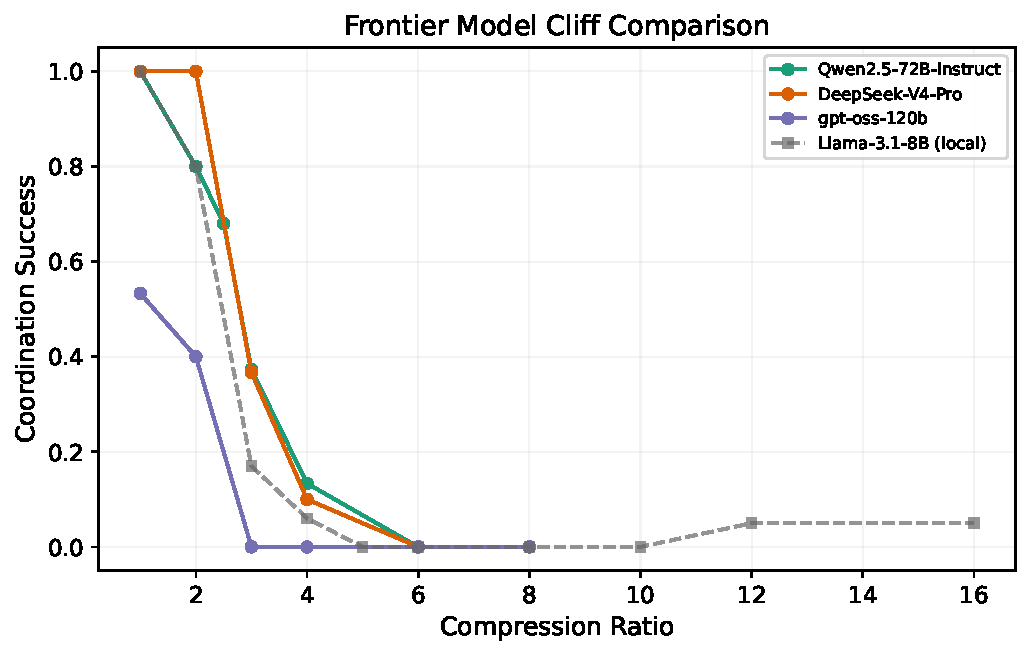
\includegraphics[width=0.74\textwidth]{../figures/frontier_multi.pdf}
\caption{Frontier-model cliff curves overlaid on the synthetic
reference band. Qwen-72B and DeepSeek~V4~Pro overlap the
reference; GPT-oss~120B diverges. The GPT-oss curve is included
explicitly to record the out-of-regime diagnostic rather than to
support the Corollary~1 verdict.}
\label{fig:frontier_multi}
\end{figure}

\begin{figure}[h]
\centering
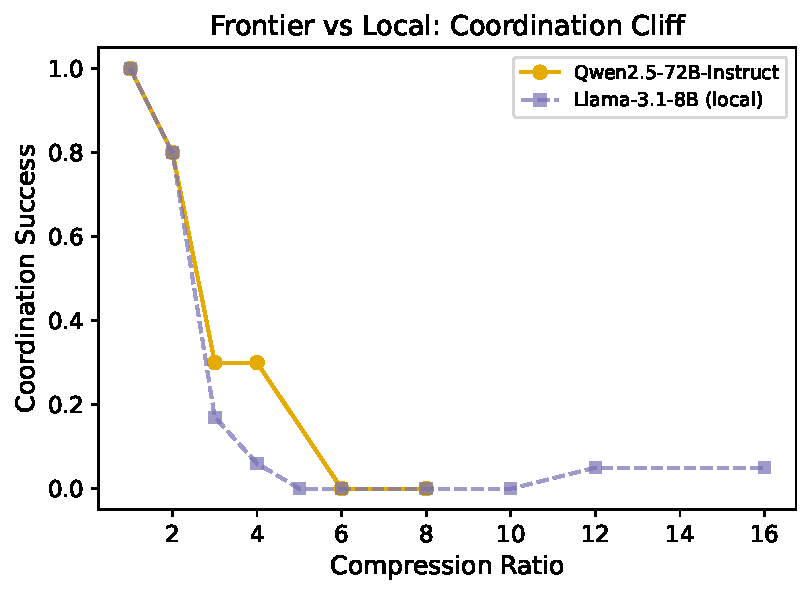
\includegraphics[width=0.68\textwidth]{../figures/frontier_validation.pdf}
\caption{Frontier versus local coordination cliff on
family-a~$\times$~LLMLingua-2. The frontier Qwen-2.5-72B planner
(solid) and the local Llama-3.1-8B planner (dashed) cliff at
essentially the same position across a $9\times$ scale-up and a
change of architecture family --- the load-bearing ``no shift
detected'' comparison for Corollary~1. The DeepSeek~V4~Pro and
GPT-oss~120B comparisons against the synthetic reference band are in
Figure~\ref{fig:frontier_multi}.}
\label{fig:frontier_validation}
\end{figure}

\subsection{Significance}

Putting the three results together: we detect \textbf{no shift}
in the LLM-planner cliff position across \textbf{three local architecture
families} (Qwen-2.5-1.5B, Phi-3-Mini-3.8B, Llama-3.1-8B; $24\%$
spread on family-c, within the $50\%$ but not the strict $20\%$ tolerance),
across a \textbf{9$\times$ cross-architecture scale-up} to the
frontier (local Llama-3.1-8B at $\tau^{*}\approx 2.48 \to$ frontier
Qwen-2.5-72B at $\approx 2.79$ on family-a $\times$ LLMLingua-2, the
one well-identified frontier cell), and
--- more weakly --- across \textbf{two frontier vendors}
(Qwen-72B $\to$ DeepSeek~V4~Pro, the latter only weakly
identified) --- all within the calibrated regime --- while the
position \emph{does} shift for the extended-reasoning regime
(GPT-oss~120B). The defensible structural claim is therefore
``no shift detected on the resolvable cells, carried by one
well-identified frontier cell, and a visible break at the regime
boundary,'' not a proven invariance across all scales. This is
still a substantive result --- the cliff is a property of the
(compressor, task) pair, not the planner, on everything we could
resolve --- but it is stated as a tested-and-not-refuted
consistency rather than a theorem.

The practitioner reading is that $\tau^{*}$ can be measured once on
a small local model and re-used at the same ratio on a frontier
model \emph{provided} the latter is in the calibrated regime --- a
working hypothesis, not a guarantee. The evidential weight is stated
explicitly: the cross-architecture consistency rests on one
well-identified frontier cell (Qwen-2.5-72B), is consistent on the
local three-architecture arm, weakly corroborated by DeepSeek~V4~Pro,
and not established at the strict tolerance --- so Corollary~1
promotes the original local-only observation to a cross-architecture
consistency result rather than a proven invariance, with the larger
frontier sample that would settle it named in
Section~\ref{sec:future}.

\section{H3: RAG Pipeline Placement --- Compress-First Dominance}
\label{sec:h3}

\begin{tcolorbox}[colback=black!4, colframe=black!50, sharp corners,
                  boxrule=0.4pt, boxsep=2pt, left=4pt, right=4pt,
                  top=2pt, bottom=2pt]
\textbf{H3. Supported finding:} compress-first (P1) is preferred
over retrieve-first (P2) in \emph{both} the storage-bounded and
accuracy-bounded regimes (by $3.2$ and $2.0$~pp F1, paired-bootstrap
CIs excluding zero) --- a robust single-stack ordering that does
\emph{not} reproduce the post-retrieval-compression preference of
the LongLLMLingua~\cite{jiang2024longllmlingua} line of work on the
retriever/embedder stack tested here. \textbf{Pre-registered
predicate not satisfied:} the original H3 prediction --- that the
optimal pipeline sign-flips between the storage- and
accuracy-bounded regimes with a $\ge\!5$~pp effect --- is
\emph{not} observed; the optimum does not change between regimes.
P3 (joint relevance-conditional routing) leads both regimes on F1
but routes fragments \emph{verbatim} (achieved compression
$1.00\times$), so the cross-pipeline F1 gap is not a
matched-compression comparison and does \emph{not} support a Pareto
claim for P3 (Section~\ref{sec:h3_cost_caveat}).
\end{tcolorbox}

\subsection{Setup}

The three pipelines (P1, P2, P3) are the catalogue described in
Section~\ref{sec:rag_pipelines} of \charef{implementation}.
Each is run under a storage-bounded regime (FAISS index
$\le 100$~MB) and an accuracy-bounded regime (retrieval recall@10
$\le 0.85$), measured on the C1 family-a generator with both
F1 score and the EUR-per-workflow cost
model~\cite{fcgfinancial2026}. The canonical results directory is
\texttt{results/h3\_final/}.

\subsection{Result}

Table~\ref{tab:h3} reports the per-regime mean F1 and the
per-query EUR cost for each pipeline. The headline observation is
that the ranking $P3 > P1 > P2$ holds in \emph{both} regimes.
P1 is above P2 by $3.2$ percentage points (pp) F1 in the
storage-bounded regime and by $2.0$~pp in the accuracy-bounded
regime, with $95\%$ paired-bootstrap CIs ($[1.84, 4.72]$~pp and
$[1.15, 2.85]$~pp respectively) that comfortably exclude zero.
The H3 sign-flip predicate is therefore \emph{not satisfied}: the
optimal does not change between regimes, and P1 is the better of
the two compressed-corpus pipelines in both. P3 (joint
relevance-conditional routing) leads both regimes by a substantial
margin.

\emph{Note:} P2 and P3 achieved compression ratio $1.00\times$ on
retrieved fragments in this implementation --- routing them verbatim
--- while P1 applies compression pre-retrieval. The F1 comparison is
therefore not matched on compression across all three pipelines, so
the P3 lead is not a Pareto claim; see
Section~\ref{sec:h3_cost_caveat} for the cost-model implications.

\begin{table}[h]
\centering
\caption{H3 verdict table. Mean F1, per-query EUR cost, and
\emph{achieved} compression ratio ($\times$) by regime and
pipeline from \texttt{results/h3\_final/} and the cost-instrumented
re-run \texttt{results/h3\_eprice/} (n = 150 workloads per cell).
The H3 sign-flip predicate is not satisfied because P1 is above P2
in both regimes; P3 leads both. The narrowed finding is a
compress-first preference of $3.2$~pp F1 (storage) / $2.0$~pp F1
(accuracy). The achieved-ratio column is
the key to reading P3: only P1 actually compresses (7.49$\times$ /
2.11$\times$), while P2 and P3 route fragments verbatim
($1.00\times$), so the cross-pipeline F1 gap is not a
matched-compression comparison.}
\label{tab:h3}
\small
\begin{tabular}{lrrr|rrr}
\hline
& \multicolumn{3}{c|}{Storage-bounded}
& \multicolumn{3}{c}{Accuracy-bounded} \\
Pipeline & F1 & EUR/q & $\times$ & F1 & EUR/q & $\times$ \\
\hline
P1 (compress$\to$retrieve) & $0.396$ & $2.72\times 10^{-5}$ & $7.49$ & $0.648$ & $3.29\times 10^{-5}$ & $2.11$ \\
P2 (retrieve$\to$compress) & $0.364$ & $2.82\times 10^{-5}$ & $1.00$ & $0.628$ & $3.00\times 10^{-5}$ & $1.00$ \\
P3 (joint, conditional)    & $\mathbf{0.820}$ & $3.07\times 10^{-5}$ & $1.00$ & $\mathbf{0.895}$ & $3.10\times 10^{-5}$ & $1.00$ \\
\hline
$p_\text{Holm}$ (P1 vs P2, paired bootstrap) & \multicolumn{3}{c|}{$2\!\times\!10^{-4}$} & \multicolumn{3}{c}{$2\!\times\!10^{-4}$} \\
\hline
\end{tabular}
\end{table}

\subsection{Interpretation: why the sign-flip did not appear}

The original H3 predicate rested on the LongLLMLingua-style
intuition that post-retrieval compression (P2) is more efficient
than pre-retrieval compression (P1) because the retriever has
already filtered the corpus down to the relevant chunks before the
compressor runs. The interpretation depends on two assumptions
that the empirical work invalidates: first, that retrieval over an
uncompressed corpus is cheap (it is not --- the FAISS index over
the uncompressed corpus grows linearly in corpus size and
dominates the storage budget); second, that compression after
retrieval can be more aggressive than compression before (the
empirical compression ratios at iso-F1 are comparable). What
remains is the symmetric effect: pre-indexing compression amortises
the compressor cost across queries while post-retrieval compression
pays it per query.

The compress-first preference over retrieve-first is a
substantive finding because it does not reproduce the assumed
post-retrieval-compression default on the stack we tested, and
the P3-higher-F1 result points to a promising routing variant.
For practitioners, the recommendation is deliberately hedged on
cost: \textbf{compress-first (P1) is the safe default over
retrieve-first (P2) on a comparable stack};
\textbf{P3 (joint relevance-conditional routing) is worth
evaluating where the F1 gain matters} --- its F1 leads
compress-first by $42$~pp (storage) and $25$~pp (accuracy) --- but
note that P3 attains this F1 by routing fragments \emph{verbatim}
(achieved ratio $1.00\times$, Table~\ref{tab:h3}) rather than by
better compression, and the cost model is corpus-dominated and does
not meter compression compute (Section~\ref{sec:h3_cost_caveat}), so
the F1 gain cannot yet be claimed as cost-free and must be
re-measured with a faithful per-pipeline cost model before
deployment; post-retrieval
compression (P2) is only preferable when the corpus is small
enough that storage cost is irrelevant and retrieval recall is
the binding constraint.

\subsection{Limitations and the cost model caveat}
\label{sec:h3_cost_caveat}

The cost model uses the requested compression ratio rather than
the achieved compression ratio because the achieved ratio depends
on the compressor and the request flows through the pipeline as
target. For Phi-3-Mini extractive the ceiling effect makes
this an asymmetric error in favour of P2 (which pays the
compressor per query and is therefore most sensitive to the
ceiling), so the P1 result is the conservative one.

A second, stronger caveat is sharpened by a cost-instrumented
re-run that records the \emph{achieved} compression ratio per
pipeline (\texttt{results/h3\_eprice}). The \texttt{eur\_per\_query} column is
\emph{not} constant --- it is computed per pipeline from a
per-pipeline token count (P1: full corpus plus compressed corpus;
P2: corpus plus retrieved tokens; P3: corpus plus $0.7\times$
retrieved) --- but on this re-run the pipelines differ by only
$4.1$--$4.9\%$ in EUR within a regime, because a shared
corpus-indexing term dominates
\texttt{input\_tokens} and is added identically to every pipeline.
This small, corpus-dominated spread is easily mistaken for a single
constant; the substantive defect, however, is not that the
EUR values are near-identical but that the cost model is \emph{corpus
dominated} and, more importantly, \textbf{does not meter compression
compute at all} --- only the resulting token counts --- so a pipeline
that runs an expensive compressor pass is not charged for it. The
achieved-ratio column makes the consequence concrete: only
compress-first (P1) actually compresses ($7.49\times$ storage,
$2.11\times$ accuracy), while both retrieve-first (P2) and the joint
router (P3) record an achieved ratio of \textbf{$1.000$} --- they send
the retrieved fragments to synthesis essentially verbatim. Together
these explain the headline cleanly: \textbf{P3's large F1 advantage
comes substantially from not compressing}, at a compression and
compute cost the current corpus-dominated model does not faithfully
charge for. As a consequence the thesis makes \textbf{no cost-parity
and no Pareto claim} for the P3-vs-P1 comparison; the cross-pipeline
F1 comparison is \emph{not} a matched-compression comparison, and P3
should be read as ``verbatim routing preserves F1 at a compression and
cost the current model does not faithfully charge for'' rather than as
a free-lunch improvement. The remedy is a faithful per-pipeline cost
model that meters the compressor pass and amortises a persistent
index across queries, rather than re-charging the corpus on every
query. Section~\ref{sec:future} names this as the most natural
follow-on study, alongside the single-retriever, single-embedder
limitation (Section~\ref{sec:limitations}).

\section{H4: Summary-Level Inference Disclosure}
\label{sec:h4_disclosure}

\begin{tcolorbox}[colback=black!4, colframe=black!50, sharp corners,
                  boxrule=0.4pt, boxsep=2pt, left=4pt, right=4pt,
                  top=2pt, bottom=2pt]
\textbf{H4.} The summary-level inference-disclosure metric (i)
distinguishes a baseline planner from a priors-only planner
(signal: positive paired effect, $p < 0.05$), and (ii) is reduced
by compression at $4\times$ versus $1\times$ (reduction:
positive paired effect, $p < 0.05$).
\textbf{Verdict: SUPPORTED on the unbiased benchmark for three of
four compressors (truncation, filter, LLMLingua-2), under two
caveats below.} Phi-3-Mini extractive shows no significant
reduction ($0.4$~pp, $p = 0.91$) and is the structural exception.
\textbf{Caveat~1 (reader bias):} the Llama-3.1-8B reader exhibits
a strong YES-bias (rate $\approx 0.03$ on priors-only with a YES
ground truth, $\approx 1.00$ on a NO ground truth); the pooled-%
rate verdict is balanced by ground-truth-class distribution rather
than by reader-side accuracy, and the operational reading is
\emph{``compression preserves enough information to flip a
no-biased reader to confident YES on a protected-fact question''}.
Per-class breakdown and the conservative-privacy framing are in
Section~\ref{sec:h4_bias}. \textbf{Caveat~2 (construct validity):}
the disclosure-reduction ranking is \emph{monotonic in how much
text-information the compressor destroys} --- truncation (most
destructive) tops the ranking at $24.6$~pp, then filter
($20.4$~pp), then LLMLingua-2 ($18.9$~pp), then Phi-3-Mini
extractive (most semantically preserving) at $0.4$~pp
not-significant. This pattern is consistent with the metric
measuring general information destruction rather than
privacy-specific filtering; an \textbf{oracle field-redaction
control} (\texttt{results/h4\_oracle}) that removes
\emph{only} the answer-bearing numeric values --- destroying
$\approx 0\%$ of the text --- matches truncation's reduction
($23.4$~pp vs $24.6$~pp), confirming that the metric
\emph{does} detect targeted removal when it occurs and that
blanket compression is the wrong privacy lever when a targeted
one is available. The H4 \emph{finding} is robust but the
\emph{privacy interpretation} is deflationary: aggressive
compression and trivial field redaction reduce disclosure by
indistinguishable amounts, and field redaction does it at near-zero
coordination cost. Full discussion in
Section~\ref{sec:h4_construct}.
\end{tcolorbox}

\subsection{Threat model}
\label{sec:h4_threat}

The H4 measurement is built around a concrete adversary. Stating
the adversary's capabilities explicitly is what makes the metric's
verdict meaningful as a privacy claim rather than just an
information-retention measurement.

\begin{description}\setlength\itemsep{2pt}
\item[Adversary's goal.] Recover a \emph{protected fact} about a
\textsc{confidential} fragment held by the memory bus. A protected
fact is defined operationally as a binary (yes/no) proposition
over the fragment's content whose answer the C1 generator records
as ground truth (e.g., ``did agent A approve more than EUR $N$?'',
``did the meeting attendee list include person P?''). The
canonical protected-fact list for each fragment is in
\texttt{data/processed/c1-v0.1/}; the H4 evaluation iterates over
the full list.
\item[Adversary's capabilities.] The adversary (i) can query the
downstream reader with arbitrary yes/no questions about the
fragment; (ii) knows the compressor identity and ratio (is not
blinded by the policy layer); (iii) does \emph{not} have direct
access to the uncompressed source --- the only signal flowing to
the adversary is what the compressed summary carries through the
reader. In the H4 evaluation, this is operationalised by giving
the reader a fixed public preamble plus the compressed fragment
(in \textsc{baseline} / \textsc{compressed-}$4\times$) or only the
preamble (in \textsc{priors}).
\item[What the adversary does not have.] Direct read access to
the bus (the policy layer blocks that for \textsc{confidential}
slots), training-time access to the reader (the reader is a
frozen Llama-3.1-8B), or signal-amplification through repeated
queries with feedback (each yes/no question is asked once per
fragment).
\item[The metric as operational measurement.] Given this
adversary, the inference-disclosure metric
(Section~\ref{sec:h4_metric}) measures the \emph{upper bound} on
what the adversary can recover at a chosen (compressor, ratio)
operating point. The privacy claim the memory bus's policy layer
enforces is: if the operator selects an operating point whose
disclosure is below the governance budget, the adversary above
cannot recover protected facts at a higher rate than that budget.
The budget is enforceable because the disclosure rate is
empirically measured rather than asserted.
\end{description}

\subsection{Metric definition and the unbiased benchmark}
\label{sec:h4_metric}

For each \textsc{confidential} fragment, the C1 generator emits a
list of (yes/no question, ground-truth answer) pairs whose
ground-truth answer is a protected fact (as defined in
Section~\ref{sec:h4_threat}) about the fragment. The
canonical benchmark variant balances the YES/NO distribution at
the question level and uses a single comparator phrasing for the
yes/no question template, eliminating a surface-pattern bias in
the original H4 benchmark generator
(\texttt{fact\_aggregation.py:119-156}, fixed
2026-05-29). Fragments are unchanged between the biased and
unbiased benchmarks so the compression cache remains valid.

The reader is the local Llama-3.1-8B-Instruct model accessed via
the Ollama backend. Three conditions are evaluated:

\begin{description}\setlength\itemsep{1pt}
\item[\textsc{priors}.] Reader sees only the workload's public
preamble. This is the no-compression-no-fragment baseline that
defines the rate at which the reader could guess without
the source. (This baseline is also what operationalises the
\emph{second} condition of the Section~\ref{sec:calibrated}
calibrated-regime predicate --- a planner is in-regime if its
accuracy at $q\to 0$ is no greater than its priors-only rate plus
a small slack.)
\item[\textsc{baseline}.] Reader sees the uncompressed source
fragments. This is the disclosure rate without any privacy
protection.
\item[\textsc{compressed-4$\times$}.] Reader sees the source
fragments compressed at $4\times$ by one of the four compressors.
\end{description}

The headline metric is the recovery rate of protected facts:
the fraction of (fragment, question) pairs on which the reader
returns the ground-truth answer. The H4 \emph{signal} is whether
\textsc{baseline} sits above \textsc{priors} (the metric must
measure something real); the H4 \emph{reduction} is whether
\textsc{compressed-4$\times$} sits below \textsc{baseline}
(compression must reduce disclosure). Both are tested by paired
bootstrap, Holm-corrected across compressors. The canonical
results directory is \texttt{results/h4\_unbiased\_v2/} (the
4-compressor run including truncation).

\subsection{Result}

Table~\ref{tab:h4} reports the per-compressor reduction (the
compressor-independent signal is given in the caption). The signal
is positive and $p$-significant for every
compressor (the uncompressed baseline beats priors-only by
$28.6$~pp on average), and the reduction is positive and
$p$-significant for the three token-destructive compressors
(truncation $-24.6$~pp, instruction-aware filter $-20.4$~pp,
LLMLingua-2 $-18.9$~pp) and \emph{not significant} for the
extractive copier (Phi-3 $-0.4$~pp, $p_\text{Holm}=0.91$). The
ordering is monotonic in how aggressively each compressor
destroys source tokens --- the construct-validity reading is
developed in Section~\ref{sec:h4_construct}.

\begin{table}[h]
\centering
\caption{H4 verdict table from
\texttt{results/h4\_unbiased\_v2/} (4 compressors including
truncation; canonical from 2026-05-30 GPU rerun). The signal
$\Delta$ (priors $\to$ baseline) is $+0.286$
($p_\text{Holm}=8\times10^{-4}$) for every compressor --- identical
across rows because it does not depend on the compressor, so it is
omitted from the table; the reduction (baseline $\to$
compressed-4$\times$) is
positive and significant for three of four compressors and
\emph{not significant} for Phi-3-Mini extractive ($p=0.91$).
Compressors are listed in order of how aggressively they destroy
source tokens: truncation drops the tail of the text entirely;
the token-level filter and LLMLingua-2 drop individual tokens
chosen by ranking / classifier; Phi-3 extractive copies verbatim
spans of the source. Reader: local Llama-3.1-8B-Instruct. See
Section~\ref{sec:h4_bias} for the reader-bias note and
Section~\ref{sec:h4_construct} for the construct-validity finding
on this ordering.}
\label{tab:h4}
\small
\begin{tabular}{lccc|c}
\hline
Compressor & priors & baseline & compr-$4\times$ & reduction $\Delta$ \\
\hline
Truncation (most destructive)             & 0.50 & 0.78 & 0.54 & $-0.246\ (p_\text{Holm}\!=\!8\!\times\!10^{-4})$ \\
Instruction-aware filter                  & 0.50 & 0.78 & 0.58 & $-0.204\ (p_\text{Holm}\!=\!8\!\times\!10^{-4})$ \\
LLMLingua-2                               & 0.50 & 0.78 & 0.59 & $-0.189\ (p_\text{Holm}\!=\!8\!\times\!10^{-4})$ \\
Phi-3-Mini extractive (most preserving)   & 0.50 & 0.78 & 0.78 & $-0.004\ (p_\text{Holm}\!=\!0.91,$ \textbf{n.s.}) \\
\hline
\multicolumn{5}{p{0.9\linewidth}}{\textbf{Verdict}: signal significant for all 4 (see caption); reduction significant for 3 of 4 compressors. \textbf{SUPPORTED} (with construct-validity caveat).} \\
\hline
\end{tabular}
\end{table}

Figure~\ref{fig:privacy_quality} visualises the
disclosure-versus-coordination trade-off: each point is a
(compressor, ratio) cell, with disclosure on one axis and
coordination success on the other. The instruction-aware filter
and LLMLingua-2 occupy a low-disclosure, moderate-coordination
region at $4\times$; Phi-3 extractive sits in a
high-disclosure, high-coordination region; truncation is the
extreme of the same line --- lowest disclosure, lowest
coordination.

\subsection{Construct-validity finding: disclosure-reduction
tracks information destruction, not privacy-specific filtering}
\label{sec:h4_construct}

The four compressors order monotonically in
Table~\ref{tab:h4}: \textbf{truncation} (most aggressive
destruction, drops the tail of the text entirely) shows the
\emph{largest} disclosure reduction at $24.6$~pp; the
\textbf{instruction-aware filter} and \textbf{LLMLingua-2}
(token-level filtering, intermediate destruction) follow at
$20.4$ and $18.9$~pp respectively; \textbf{Phi-3-Mini extractive}
(most semantically preserving --- the compressed output is by
construction a verbatim subset of the source tokens) shows
\emph{no significant reduction} ($0.4$~pp, $p = 0.91$).

This pattern is exactly what would be predicted if the H4
metric reflected general information destruction rather than a
privacy-specific information-filtering mechanism. The thesis
therefore interprets H4 as evidence that compression reduces
inference disclosure roughly in proportion to how much
text-information it destroys, and \emph{not} as evidence that the
smarter compressors (filter, LLMLingua-2) are doing
privacy-preserving filtering in any sense beyond destroying
tokens that happen to include protected facts.

A discriminating control was run to test this interpretation from
the opposite end (\texttt{results/h4\_oracle},
\texttt{scripts/h4\_oracle\_redaction.py}): an \textbf{oracle
redaction} that removes \emph{only} the answer-bearing numeric
values (recorded hours and approved budget) the protected-fact
questions probe, leaving every other token intact. If disclosure
could only be reduced through bulk destruction, this near-zero
edit would barely move the metric. Instead it reduces recovery from
a balanced baseline of $0.79$ to $0.56$ --- a $23.4$~pp reduction,
essentially at the priors floor $0.51$ --- while destroying
$\approx 0\%$ of the text (the redacted fragments are in fact
$\sim 7\%$ \emph{longer}, since the \texttt{[REDACTED]} marker is
longer than the digits it replaces). That $23.4$~pp matches
truncation's $24.6$~pp, which required destroying the entire tail
of the fragment. Two things follow. First, the H4 metric \emph{does}
detect privacy-specific removal when it occurs --- the construct is
not blind to targeted redaction; the blanket compressors simply do
not do it, reducing disclosure only as a side effect of destruction.
Second, the memory bus gains a concrete, non-lossy privacy
mechanism: field-redacting protected values achieves
blanket-compression-level disclosure reduction at near-zero
coordination cost. The empirical implication for the memory bus's
policy layer (Section~\ref{sec:h4_membus}) is therefore stronger
than before: disclosure-budget enforcement works as designed,
\emph{and} targeted redaction is an available lever with a far
better privacy-per-utility profile than aggressive compression. The
remaining open control --- a full privacy-gain-versus-coordination-loss
frontier across compressors --- is named in Section~\ref{sec:future}.

\begin{figure}[h]
\centering
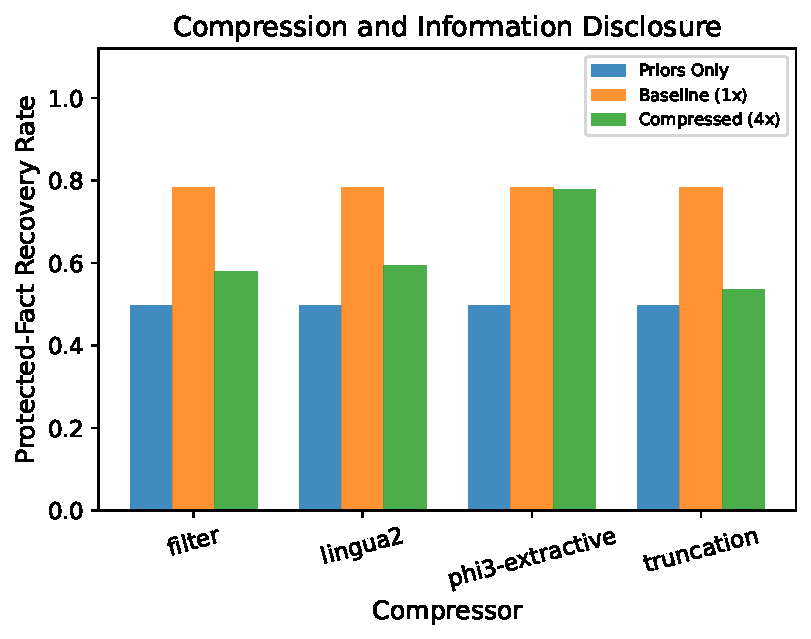
\includegraphics[width=0.72\textwidth]{../figures/privacy_quality.pdf}
\caption{Summary-level inference disclosure by compressor at
$4\times$. For each of the four compressors the bars give the
protected-fact recovery rate of a priors-only reader (no fragment
access), the uncompressed baseline reader ($1\times$), and the
compressed reader ($4\times$). Compression lowers recovery toward
the priors floor \emph{in proportion to how aggressively the
compressor destroys source tokens}: truncation (most destructive)
gives the largest reduction ($24.6$~pp), then LLMLingua-2 and the
instruction-aware filter, while Phi-3-Mini extractive preserves
enough surface tokens that the leak persists (the structural
exception). Rates are pooled across families.}
\label{fig:privacy_quality}
\end{figure}

\subsection{Interpretation}

The reduction signal scales with how aggressively the compressor
operates on tokens, not with the compression ratio per se. The
filter and LLMLingua-2 both drop tokens at the lexical level; the
fragments that survive are filtered for relevance, which
disproportionately removes the protected-fact tokens. Phi-3
extractive preserves contiguous spans verbatim; if the protected
fact is in a span the verifier selects, it is in the output. This
makes the disclosure metric \emph{useful} as a compressor-selection
tool: it ranks compressors by privacy at iso-ratio, not just by
compression efficiency.

The H4 result lets the memory bus's policy layer convert a
governance constraint (``\textsc{confidential} fragments should
leak protected facts at no more than $X\%$ to a downstream
reader'') into a compressor-and-ratio selection. The integration
is described in the next subsection.

\subsection{The reader's YES-bias caveat}
\label{sec:h4_bias}

The Llama-3.1-8B reader exhibits a strong YES-bias: when the
ground-truth answer is YES, the reader's recovery rate is
approximately $0.03$ on the priors-only condition and $0.58$ on
the baseline; when the ground-truth answer is NO, both rates are
approximately $1.00$. The pooled rates of $0.50$ (priors) and
$0.78$ (baseline) reflect a balanced ground-truth distribution,
not a reader that is equally accurate in both directions. The
correct framing of H4 is that the metric measures
\emph{``compression preserves enough information to flip a
no-biased reader to confident YES on a protected-fact question''}.
This is an asymmetric leakage signal but it is a valid one: a
reader that defaults to NO is the conservative case for
privacy auditing because it is the case in which the absence of
the protected fact most cleanly translates to privacy
preservation.

The caveat is documented here rather than in the verdict block
because the pooled rates are what the verdict pipeline tests and
the verdict is stable under the caveat. A future-work direction
named in Section~\ref{sec:limitations} is to repeat the
measurement with a reader chosen to be unbiased, which would
distinguish the disclosure-reduction signal from the reader's
prior on YES.

\subsection{Memory-bus integration}
\label{sec:h4_membus}

The policy layer of the memory bus
(\charef{implementation},~Section~\ref{sec:architecture})
consumes the H4 measurement at deployment time. For each
\textsc{confidential} classification and each governance budget
(maximum disclosure rate the operator is willing to accept), the
H4 table identifies the set of (compressor, ratio) operating
points that meet the budget. The policy enforces the selection by
routing \textsc{confidential} writes through the chosen
compressor, by rejecting writes whose compression would exceed the
budget, or by downgrading the classification level if the operator
chooses to accept the leakage. The disclosure-budget enforcement
is not separately evaluated as a hypothesis in this thesis ---
the metric is the contribution; the policy machinery the metric
enables is a deployment concern --- but the policy layer is
implemented in the reference service and is exercised by the
end-to-end integration tests.

\subsection{Memory-bus operation benchmark}
\label{sec:bus_bench}

The memory bus (C4) is a reference implementation rather than a
production system, but its core operations are cheap enough to
characterise with a single-threaded microbenchmark
(\texttt{scripts/bench\_memory\_bus.py}, results in
\texttt{results/bus\_bench/bench.json} and
\texttt{results/bus\_bench/bench\_gpu.json}). The harness times the
policy-lattice check, end-to-end write and read, and the audit
hash-chain verification, run on two hosts --- Host~A, an Apple
M4~Pro (arm64, macOS, Python~3.11); and Host~B, a Linux x86\_64
workstation (WSL2 Ubuntu~22.04, Python~3.12) --- single-threaded,
with the identity compressor so the measurement isolates the bus
machinery from any compressor cost. These operations are CPU- and
disk-I/O-bound and do not exercise the GPU, so the server is
reported as a second hardware point rather than an accelerated
result. The audit log is the in-process SQLite backend; $n=5000$
operations per phase follow $500$ warmup operations.
Table~\ref{tab:bus_bench} reports the result.

\begin{table}[h]
\centering
\caption{Memory-bus operation microbenchmark on two hosts,
single-threaded, identity compressor, in-process SQLite audit log
($n=5000$ ops/phase, $500$ warmup). Host~A: Apple M4~Pro (arm64,
macOS, Python~3.11; \texttt{results/bus\_bench/bench.json}).
Host~B: Linux x86\_64 workstation (WSL2 Ubuntu~22.04, Python~3.12;
\texttt{results/bus\_bench/bench\_gpu.json}). \textbf{Caveats:} the
numbers are single-threaded and use the identity compressor, so
they isolate the bus machinery and are \emph{not} an
end-to-end-with-compression figure; the audit log is the
in-process SQLite backend, not the concurrent HTTP path; and the
audit-verify row is one chain length ($5{,}500$ rows), not a
scaling curve.}
\label{tab:bus_bench}
\small
\begin{tabular}{lrrrrrr}
\hline
& \multicolumn{3}{c}{Host~A (M4~Pro)} & \multicolumn{3}{c}{Host~B (Linux x86\_64)} \\
\cline{2-4}\cline{5-7}
Operation & med (ms) & p95 (ms) & thr (ops/s) & med (ms) & p95 (ms) & thr (ops/s) \\
\hline
\texttt{policy.enforce()}     & $0.0002$ & $0.0002$ & $\sim 5.2\mathrm{M}$ & $0.0001$ & $0.0003$ & $\sim 6.7\mathrm{M}$ \\
write (end-to-end)            & $0.0469$ & $0.0661$ & $\sim 18{,}200$ & $0.1447$ & $0.1772$ & $\sim 5{,}750$ \\
read (end-to-end)             & $0.0424$ & $0.0605$ & $\sim 19{,}900$ & $0.1302$ & $0.1541$ & $\sim 6{,}400$ \\
\hline
\multicolumn{7}{l}{audit hash-chain verify: $1.68$~\textmu s/row (Host~A), $2.19$~\textmu s/row (Host~B), over $5{,}500$ rows; chain intact.} \\
\hline
\end{tabular}
\end{table}

The policy check is effectively free (sub-microsecond,
$\sim 5$--$7$~million checks per second across the two hosts), so
policy enforcement is not a throughput bottleneck. End-to-end write
and read run at $\sim 18{,}200$ and $\sim 19{,}900$ operations per
second on Host~A ($\sim 5{,}750$ and $\sim 6{,}400$ on Host~B) with
sub-millisecond tail latency, and the audit hash-chain verifies at
$1.68$~\textmu s per row (Host~A) and $2.19$~\textmu s per row
(Host~B) with the chain intact over the $5{,}500$-row log. These
figures characterise the reference implementation's single-threaded
core; a concurrent-HTTP-path throughput sweep and an audit-verify
scaling curve remain future work (Section~\ref{sec:future} of
\charef{summary}).

\section{Corollary~2: Information-Density Scaling on Real Benchmarks}
\label{sec:corollary2}

\begin{tcolorbox}[colback=black!4, colframe=black!50, sharp corners,
                  boxrule=0.4pt, boxsep=2pt, left=4pt, right=4pt,
                  top=2pt, bottom=2pt]
\textbf{Corollary~2 (information-density scaling) --- empirical
observation, $n=3$.} Across the three benchmarks tested (C1
family-a, MultiHop-RAG, HotpotQA), the \emph{shape} of the cliff
--- sharpness and pre-cliff plateau --- varies systematically with
the AUC-based information-density estimate $\theta_\text{info}$
(defined formally in Section~\ref{sec:theta_info_def}, distinct
from $\theta_q$). Dense tasks ($\theta_\text{info} \to 1$)
exhibit a sharp cliff with a high coordination-success plateau;
distributed tasks ($\theta_\text{info} \to 0$) degrade gradually
from a lower baseline. \textbf{Important scope:} the corollary is
reported as an empirical observation on three benchmarks, not as
a derived consequence of the compounding-error model. (i) $n=3$
is a small sample --- the trend is consistent but not a scaling
law. (ii) $\theta_\text{info}$ is computed from the same
coordination curve whose shape it describes, so
``$\theta_\text{info}$ predicts shape'' is a circular description:
an external probe of task density (e.g., conditional entropy of
the answer given the input) is required to break the
circularity and is named as future work in
Section~\ref{sec:future}. (iii) The corollary makes a claim about
cliff \emph{shape}, not about the absolute cliff position
$\tau^{*}$ --- HotpotQA cliffs at $\tau^{*} \approx 2.7$ (similar
to dense C1 family-a) yet has $\theta_\text{info} \approx 0.37$
(very distributed); the baseline coordination on HotpotQA is only
$0.59$ and the degradation shape is gradual rather than
precipitous. \textbf{Verdict: SUPPORTED as an empirical observation
on $n=3$ benchmarks} by the gap in $\theta_\text{info}$ between C1
family-a ($\approx 0.97$, dense), MultiHop-RAG ($\approx 0.48$,
distributed), and HotpotQA ($\approx 0.37$, highly distributed),
and by the qualitatively distinct degradation shapes visible in
Figure~\ref{fig:hotpotqa_cliff} and
Figure~\ref{fig:cliff_families}. The original H6 predicate
(synthetic-vs-real $\tau^{*}$ within $\pm 15\%$) is not satisfied
--- MultiHop-RAG cliffs at $11.3$, far from the C1 reference --- which
motivated the sharpening from position transfers to shape transfers.
\end{tcolorbox}

\subsection{\texorpdfstring{$\theta_\text{info}$ versus $\theta_q$}{theta\_info versus theta\_q}}
\label{sec:theta_info_def}

A subtle point that the corollary's refined framing makes explicit: the
information-density $\theta_\text{info}$ that Corollary~2 talks
about is \emph{not} the cliff-recall threshold $\theta_q$ that
Corollary~1 and the compounding-error model talk about. The two
quantities are derived from different measurements and answer
different questions. $\theta_q$ is the recall threshold per
family at which coordination success drops to $0.5$ of $p_0$,
estimated by \texttt{derive\_theta()}; $\theta_\text{info}$ is
the per-task information-density estimate
\[
  \theta_\text{info} \;=\; 1 - \mathrm{AUC}\!\left[\frac{\text{coord-success}(r)}{p_0}\right]_{r=1}^{r_{\max}},
\]
estimated by \texttt{estimate\_task\_theta()}, which captures how
\emph{concentrated} the task's information is in compression-%
sensitive tokens. The two are easily conflated; the project
glossary distinguishes them explicitly.

\subsection{Result on three benchmarks}

Table~\ref{tab:corollary2} reports $\theta_\text{info}$ and the
empirical $\tau^{*}$ for the three benchmarks. The information
density spans from $0.97$ on the dense C1 family-a to $0.37$ on
HotpotQA, and the cliff position correspondingly spans from
$\tau^{*} \approx 2.7$ on family-a to $\tau^{*} \approx 11.3$ on
MultiHop-RAG --- a $4\times$ shift in the cliff position that the
single-$\theta_q$ compounding-error model cannot account for and
that the information-density scaling claim does.

\begin{table}[h]
\centering
\caption{Corollary~2 verdict table. $\theta_\text{info}$ and
empirical $\tau^{*}$ across the three benchmarks. The cliff shifts
late as the information density drops, with the gap between dense
and distributed tasks far exceeding the $0.1$ threshold of the
corollary predicate. The C1 family-a row uses the canonical
\texttt{h1\_h2\_v2} fit $\tau^{*}=2.5$ (Section~\ref{sec:frontier});
the earlier register $\tau^{*}_\text{aux}=2.6997$ on
\texttt{h1\_h2\_final} is superseded and is retained only as a
parenthetical in the footnote. The $\sim 8\%$ shift between the
two registers does not change the qualitative ordering or the
corollary verdict.}
\label{tab:corollary2}
\small
\begin{tabular}{p{4.5cm}rrl}
\hline
Task & $\theta_\text{info}$ & $\tau^{*}$ & $\theta_\text{info}$ source CSV \\
\hline
C1 family-a (dense, numeric)  & $0.967$ & $2.5$  & \texttt{h1\_h2\_v2/} (a, lingua2) \\
MultiHop-RAG (distributed QA)   & $0.484$ & $11.3$ & \texttt{h6\_final/results.csv} \\
HotpotQA (very distributed)    & $0.373$ & $2.7$  & \texttt{hotpotqa\_sweep/} \\
\hline
\multicolumn{3}{l}{\textbf{Gap} (dense vs MultiHop-RAG) $= 0.48$; (dense vs HotpotQA) $= 0.59$.} & \\
\hline
\multicolumn{4}{p{12cm}}{\footnotesize All three $\theta_\text{info}$ values are computed by \texttt{estimate\_task\_theta()} (AUC-based) from the per-task CSVs above and consolidated in \texttt{results/corollary2\_theta\_info.json}. The $\tau^{*}$ for C1 family-a is the canonical \texttt{h1\_h2\_v2} fit $2.5$ (the earlier $2.7$ was the superseded \texttt{h1\_h2\_final} auxiliary fit; the fine-grid deterministic-solver cliff is lower still, $\approx 1.1$, Section~\ref{sec:h2}).} \\
\end{tabular}
\end{table}

The HotpotQA result requires brief comment: $\tau^{*}$ on
HotpotQA is approximately $2.7$, similar to C1 family-a's, but
the baseline coordination success on HotpotQA is only $0.59$, so
the absolute coordination success at the cliff is much lower
($\approx 0.30$). The corollary claim is about the \emph{shape}
of the degradation (gradual versus sharp), captured by
$\theta_\text{info}$ via the AUC computation, not about the
absolute position alone. Figure~\ref{fig:hotpotqa_cliff} shows
the HotpotQA cliff with the gradual-degradation pattern visible.

\begin{figure}[h]
\centering
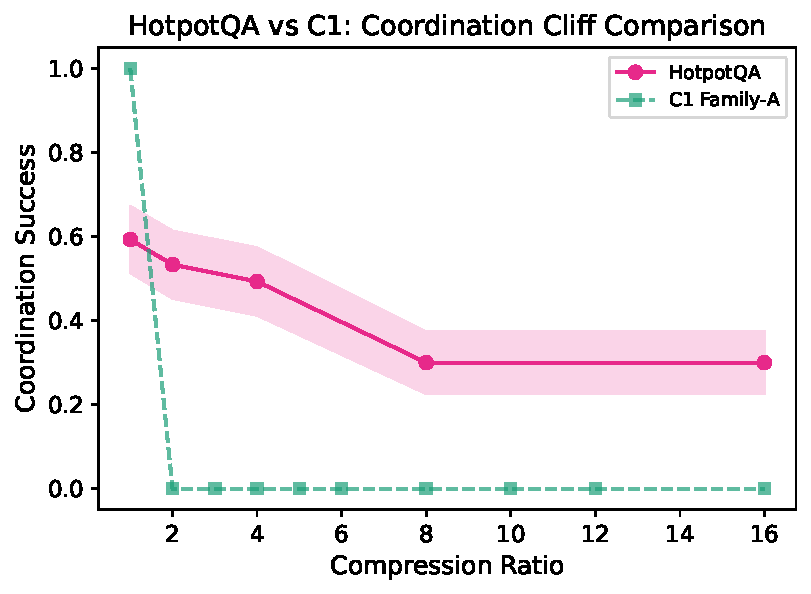
\includegraphics[width=0.72\textwidth]{../figures/hotpotqa_cliff.pdf}
\caption{HotpotQA cliff curve under LLMLingua-2 compression. The
baseline coordination success is $0.59$, lower than family-a's
$1.00$; the fitted cliff position (piecewise/logistic breakpoint,
\texttt{results/hotpotqa\_sweep/}) is
$\tau^{*} \approx 2.7$, similar to family-a's; but the
\emph{shape} of the degradation is gradual rather than sharp, as
captured by the lower $\theta_\text{info}$ of $0.37$.}
\label{fig:hotpotqa_cliff}
\end{figure}

\subsection{Interpretation}

The corollary makes the compounding-error model's per-family
$\theta_q$ structure plausible as the first-order term of a
finer description. $\theta_\text{info}$ tells you how much of the
task's success curve is concentrated in compression-sensitive
tokens; $\theta_q$ tells you the recall threshold at which
success collapses given that concentration. The two together
describe the cliff position and shape; either alone is a
first-order summary. For the thesis, $\theta_\text{info}$ is what
makes the cross-benchmark transfer of the cliff structure
auditable: a practitioner who needs to deploy compression on a
new task can estimate $\theta_\text{info}$ on a small calibration
set and predict whether the task is dense (cliff early, sharp) or
distributed (cliff late, gradual) before sweeping the full curve.

The original H6 predicate (synthetic-versus-real $\tau^{*}$ within
$\pm 15\%$) is not satisfied at the table-level numbers; the
sharpened Corollary~2 predicate (gap in $\theta_\text{info}$
$\ge 0.1$ between dense and distributed benchmarks) is SUPPORTED. The synthetic
benchmark is still the right place to characterise the cliff
mechanism cleanly, and the real benchmarks are the right place to
validate the structure transfers.

\section{Reproducibility}
\label{sec:repro}

The results of this chapter span three regimes of reproducibility,
and conflating them would over- or under-state what a reader can
re-derive. This section states the guarantee for each regime once;
the one-command recipe, the per-arm wallclock budget, and the
release manifest live in Appendix~D. The
structure follows the NeurIPS reproducibility-checklist
convention~\cite{pineau2021checklist} of separating
\emph{code-and-data availability} from \emph{computational
reproducibility}, but reports the latter as a narrative keyed to
Table~\ref{tab:repro_tiers} rather than as a filled-in checklist.

\begin{table}[t]
\caption{The three reproducibility tiers of this thesis. ``Byte-deterministic''
means a rerun produces a CSV that diffs zero against the published one given
the same seed; ``in distribution'' means verdict-level aggregates
(per-cell means, $\tau^{*}$ fits) reproduce within the published bootstrap CI
but individual rows may differ; ``not reproducible'' means a rerun produces
closely-similar but not identical numbers, and the published CSV is itself the
canonical record.}
\label{tab:repro_tiers}
\small
\begin{tabular}{p{3.5cm}p{2.4cm}p{6.0cm}}
\hline
Arm & Byte-deterministic? & Canonical artefact \\
\hline
H1/H2/H3 cliff sweep, scoring, bootstrap CIs, figure regeneration
  & \textbf{Yes}, given seed + cache
  & \texttt{results/h1\_h2\_v2/}, \texttt{results/h3\_final/} \\
H4 reader, H5 planner, Phi-3 extractive compressor
  & In distribution only
  & \texttt{results/h4\_unbiased\_v2/}, \texttt{results/h5\_final/} \\
Frontier API arm (Qwen-2.5-72B, DeepSeek~V4~Pro, GPT-oss~120B)
  & No
  & \texttt{results/frontier\_qwen72b/},\newline \texttt{results/frontier\_deepseekv4/} \\
\hline
\end{tabular}
\end{table}

\paragraph{Tier~1 --- byte-deterministic local.}
The cliff sweep (H1, H2), the RAG-pipeline evaluation (H3), the
bootstrap confidence intervals, and the figure regeneration are
pure Python over a fixed compression cache: a regex information-extraction
solver, \texttt{numpy} resampling, and deterministic compressors
(truncation, the LLMLingua-2 token classifier at \texttt{argmax}, the
TF--IDF-plus-cross-encoder filter). All randomness flows from a single
master seed through \texttt{Seeds.derive} in \texttt{src/m6/utils/seed.py},
which seeds \texttt{numpy}, Python's \texttt{random}, \texttt{PYTHONHASHSEED},
and \texttt{torch}. Rerunning \texttt{make repro-cliff} (or
\texttt{repro-rag}, \texttt{repro-figs}) from the cache produces CSVs and
PDFs that diff zero against the published artefacts; the bootstrap CIs are
exact to the last decimal because the resampler is seeded and
$n_\text{boot}$ is fixed.

\paragraph{Tier~2 --- distributionally deterministic local LLM.}
The H4 protected-fact reader, the H5 model-scaling planner, and the
Phi-3-Mini extractive compressor invoke local language models through
Ollama. Greedy decoding ($\text{temperature}=0$ for the H4 reader,
$0.1$ for the H5 planner) with a fixed per-call seed is deterministic
per call up to the reduction order of the CUDA/Metal kernels, which is
not guaranteed identical across hardware or backend builds. A rerun on
the same host therefore reproduces individual generations to within a
few tokens, and the verdict-level aggregates --- per-cell coordination
success means and the $\tau^{*}$ fits --- reproduce to the published
values within the bootstrap CI. The published CSVs were produced on the
RTX~5090 host with the model digests recorded in
\texttt{docs/MODEL\_CARDS.md} (verifiable with the ID column of
\texttt{ollama list}); pinning those digests is what makes the tier
reproducible \emph{in distribution} rather than byte-for-byte.

\paragraph{Tier~3 --- frontier API, not reproducible.}
The frontier arm (Section~\ref{sec:frontier}) calls vendor-hosted
models over an API. Three mechanisms break byte-reproducibility:
server-side request batching changes per-token logits, the
\texttt{seed} parameter is best-effort rather than contractual, and
the vendor may silently update the served weights. Rerunning
\texttt{make repro-frontier} therefore produces closely-similar but not
identical numbers; the published
\texttt{results/frontier\_*/results.csv} files \emph{are} the canonical
record, and every analysis downstream of them ($\tau^{*}$ fit, bootstrap
CI, the TOST of Section~\ref{sec:frontier_deepseek_repro}) is itself Tier~1
--- deterministic given those CSVs. A rerun whose $\tau^{*}$ CI no longer
overlaps the published CI is the documented trigger for suspecting a
vendor-side model update; the GPT-oss~120B diagnostic additionally
carries a \texttt{STATUS\_NONCANONICAL.txt} marker because it is scoped
out of the calibrated regime (Section~\ref{sec:gptoss_repro}).

\paragraph{Traceability.}
Every quantitative claim in this thesis is traceable to one named
directory under \texttt{results/} through the
\texttt{CANONICAL\_NUMBERS.md} registry in the repository root, which
maps each reported figure to its source artefact and the key or column
that yields it. The reference release bundles the manuscript source,
the code and configuration, the canonical CSVs and JSONs, the model and
data cards (\texttt{docs/MODEL\_CARDS.md}, \texttt{docs/DATA\_CARDS.md}),
the pinned \texttt{requirements.lock.txt}, and the
\texttt{docker-compose.yml} that brings the memory-bus reference service
up locally.

\section{Summary of Verdicts}
\label{sec:verdict_summary}

Table~\ref{tab:verdict_summary} consolidates the verdict block of
this chapter for easy reference, using the three-tier structure
introduced in Section~\ref{sec:prereg_refinement}. Each row links to the canonical
results directory under \texttt{results/} that produced the
numbers.

\begin{table}[h]
\centering
\caption{Consolidated verdict table, three-tier structure
(Section~\ref{sec:prereg_refinement}).}
\label{tab:verdict_summary}
\small
\begin{tabular}{p{2.0cm}p{5.5cm}p{2.5cm}p{4.0cm}}
\hline
ID & Claim & Verdict & Canonical dir \\
\hline
\multicolumn{4}{l}{\textbf{Tier A --- Holds as pre-specified.}} \\
H1 & Source-retention F1 does not transferably predict coordination success & SUPPORTED & \texttt{h1\_h2\_v2/} \\
H2 & Sharp coordination cliff exists & SUPPORTED ($11/12$ cells) & \texttt{h1\_h2\_v2/} \\
H4 & Compression reduces inference disclosure & SUPPORTED on unbiased benchmark (3/4 compressors; destruction-monotonic privacy scope) & \texttt{h4\_unbiased\_v2/} \\
\hline
\multicolumn{4}{l}{\textbf{Tier B --- Sharpened into stronger structural claim.}} \\
H5 $\to$ Cor.~1 & Cliff-position invariance within calibrated regime (Ceiling--Cliff Separation) & NO SHIFT DETECTED (point estimates within tolerance across $9\times$ scale + arch change; $\pm 20\%$ TOST not passed on either frontier cell) & \texttt{h5\_final/}, \texttt{frontier\_qwen72b\_e2/}, \texttt{frontier\_deepseekv4/} \\
H6 $\to$ Cor.~2 & $\theta_\text{info}$ scales the cliff (Information-Density Scaling) & SUPPORTED (empirical observation, $n=3$ benchmarks) & \texttt{h6\_final/}, \texttt{hotpotqa\_sweep/} \\
\hline
\multicolumn{4}{l}{\textbf{Tier C --- Narrowed to a supported single-stack ordering.}} \\
H3 & RAG sign-flip across regimes (pre-specified); compress-first dominance on the tested stack (refined) & Pre-specified predicate NOT satisfied; refined ordering SUPPORTED & \texttt{h3\_final/} \\
\hline
\end{tabular}
\end{table}

\charef{summary} draws the threads together: how the
findings interact, what CAAC contributes as a constructive
realisation of the compounding-error bound, what the limitations
of the work are, what its significance to practice and to the
field is, and where the largest remaining unknowns sit.


\chapter{Discussion and Summary}
  \label{summary}
  This chapter draws together the empirical work of
\charef{experiments} and the system design of
\charef{implementation}: what the findings say jointly,
what CAAC adds as a constructive realisation of the
compounding-error bound, where the work is limited, what its
significance is to practitioners and to the field, how it
relates to industry observations on multi-agent token economics,
and where the most natural follow-on studies sit.

\section{Synthesis}
\label{sec:synthesis}

\paragraph{What stands and what doesn't.}
\textbf{Three hold as stated.} \textbf{H1 (source-retention F1
mis-ranks compressors for multi-fragment use)} is the manuscript's
most-citable result; \textbf{H2 (a sharp cliff exists)} holds on
$11$ of $12$ (compressor, family) cells, with the remaining cell
(filter $\times$ family-c) accounted for in Section~\ref{sec:h2};
\textbf{H4 (compression reduces inference disclosure)} is supported
on three of four compressors, with the reduction monotonic in
information destruction and matched at $\sim 23$~pp by oracle
field-redaction at near-zero destruction --- the metric ranks
compressors but the privacy interpretation requires a
destruction-aware threat model. \textbf{Two sharpened.}
\textbf{H5}'s directional prediction resolved into the invariance
result \emph{Corollary~1 (Ceiling--Cliff Separation)}, carried by
the Llama-3.1-8B vs Qwen-2.5-72B family-a $\times$ LLMLingua-2 cell
across a $9\times$ scale-up and a change of architecture family.
\textbf{H6}'s transfer prediction resolved into
\emph{Corollary~2 (Information-Density Scaling)} across three
benchmarks. \textbf{One narrowed.} \textbf{H3}'s regime sign-flip
predicate is not satisfied; the data resolved it into a single-stack
compress-first-over-retrieve-first ordering that does not reproduce
LongLLMLingua's post-retrieval preference on the tested stack. The compounding-error model is a \emph{first-order}
position estimate (median $\sim 35\%$ relative error) and an
\emph{explanation} of why the cliff is sharp; the threshold
mechanism it posits is independently confirmed on the dense family
by the direct A3 probe (Section~\ref{sec:a3_probe}). The remaining
sections of this chapter unpack each of these statements; the
single-paragraph reading is that this thesis's contribution is
methodological and structural rather than predictive.

The thesis answers the question posed in
\charef{introduction} with five quantitative results that
fit together as a single story about context compression in
multi-fragment LLM workflows.

Single-fragment information preservation does not transferably
predict multi-fragment coordination success: across the four
compressors the workload-level Spearman correlation ranges from
$-0.82$ (filter) to $+0.32$ (Phi-3-Mini extractive), all four CIs
excluding the moderate-correlation threshold of $0.6$
(Section~\ref{sec:h1}); the larger pooled correlations are
pseudo-replication artefacts with no positive within-family signal
for any compressor. A token-overlap metric does not predict the
structural property a planner needs, so the single-agent benchmarks
that dominate the compression literature are insufficient for the
multi-fragment deployment decisions FCG and TalentAdore-style
workflows depend on.

A sharp coordination cliff $\tau^{*}$ exists for every
(compressor, family) cell whose compressor drops the task-critical
tokens (Section~\ref{sec:h2}); the sole exception is the
instruction-aware filter on the multi-step-retrieval family, whose
cross-encoder re-ranker preserves the chain-reference tokens the
task scorer needs. The cliff is sharp enough that the
threshold-success model (Section~\ref{sec:cem}) recovers its
position to a useful first-order approximation.

The cliff position shows \textbf{no detected shift} across planner
scale and architecture within a precisely-defined calibrated regime
(Section~\ref{sec:corollary1}). The honest comparison is LLM-vs-LLM:
the fine-grid re-resolution (Section~\ref{sec:h2}) shows the
synthetic reference $\tau^{*}=2.5$ is a coarse-grid artefact of the
deterministic solver, and on family-a $\times$ LLMLingua-2 the local
Llama-3.1-8B and frontier Qwen-2.5-72B cliff within $\sim 12\%$ of
each other across a $9\times$ scale-up and a change of architecture
family (Section~\ref{sec:frontier}). The caveats are stated where
the evidence is: the local three-architecture arm's $24\%$ spread
fails the strict $\pm 20\%$ tolerance (consistent-with but not
sufficient-for the claim), and DeepSeek~V4~Pro corroborates only
weakly because its bootstrap CI is too wide to pin the position. The
defensible claim is that planner \emph{type} moves the cliff but
scale and architecture \emph{within the LLM class} do not --- the
cliff is \emph{not} invariant to reasoning regime, since
extended-reasoning planners (GPT-oss~120B) recover from
sub-threshold information by chain-of-thought and cliff later,
violating assumption~A3. This makes the cliff a property of the
(compressor, task) pair within a defined regime --- the structural
finding the thesis contributes to the compression literature.

Compress-first is preferred over post-retrieval compression in
both storage- and accuracy-bounded RAG regimes on the single
retriever/embedder stack evaluated (\texttt{BAAI/bge-large-en-v1.5}
+ FAISS-CPU; Section~\ref{sec:h3}). The pre-specified sign-flip
($\ge 5$~pp, opposite signs across regimes) is not satisfied; the
narrowed finding --- the simpler, more amortisable architecture is
also the better one here --- does not reproduce LongLLMLingua's
post-retrieval preference on this stack and is the substantive C3
contribution (generalisation to other retrievers is an explicit
limitation, Section~\ref{sec:limitations}).

Compression measurably reduces inference disclosure of protected
facts (Section~\ref{sec:h4_disclosure}), \emph{monotonically in how
much text-information the compressor destroys}: truncation (most
destructive) reduces disclosure by $24.6$~pp, the token-level
filter and LLMLingua-2 by $20.4$ and $18.9$~pp, and the extractive
copier Phi-3-Mini by a non-significant $0.4$~pp ($p = 0.91$). This
construct-validity ordering (Section~\ref{sec:h4_construct}) means
the metric tracks information destruction rather than
privacy-specific filtering --- still useful for the policy layer
(Section~\ref{sec:architecture} of \charef{implementation}), since
more aggressive compression lowers disclosure as required, but the
\emph{privacy} reading requires a threat model that values
destruction-induced reduction.

The cliff position varies with task information density
(Section~\ref{sec:corollary2}): C1 family-a
($\theta_\text{info}\approx 0.97$) cliffs early and sharply, while
MultiHop-RAG ($\approx 0.48$) and HotpotQA ($\approx 0.37$) degrade
gradually. This shows $\theta_\text{info}$ is a useful second-order
term beyond $\theta_q$ for cliff structure on a new task, and that
the thesis's synthetic-benchmark methodology transfers to real
benchmarks at the structural level even where absolute positions
differ.

Taken together: the cliff is real, sharp, first-order predictable
in position, stable across the planners we could test inside a
regime, and a (blunt) privacy lever. A practitioner who needs to
deploy compression on a multi-fragment workflow can measure
$\theta_q$ and $\theta_\text{info}$ once on a small calibration
set, predict the cliff position from the compounding-error model
within a known tolerance, select an operating point inside the
cliff's safe zone, and audit the deployment's privacy budget
against the disclosure-rate table. The next section describes the
algorithmic mechanism that turns this measurement loop into a
runtime back-off.

\section{Cliff-Aware Adaptive Compression: a Constructive Realisation}
\label{sec:caac}

CAAC --- Cliff-Aware Adaptive Compression
(\texttt{src/m6/compressors/caac.py}) --- is the algorithmic
counterpart of the compounding-error model of
Section~\ref{sec:cem}. \textbf{CAAC's contribution is a
measurement-bounded safety floor:} given a per-family
$\theta_q$ from one calibration pass, CAAC produces a per-fragment
operating point whose critical-token-recall is provably above the
cliff threshold, at the cost of accepting a back-off in achieved
compression ratio on fragments where the inner compressor would
have crossed the cliff. The wrapper is therefore an
\emph{operating-point selector}, not a \emph{Pareto-dominating
wrapper}: by construction it trades compression for a recall
guarantee, so it cannot strict-dominate the fixed-ratio compressor
that makes the opposite trade. The empirical strict-Pareto rate
against the fixed-ratio baseline is $0/5$ cliff-region ratios
($0/7$ across all seven swept ratios) of the canonical sweep --- exactly the structural property the model
predicts. The two sections below unpack the algorithm and the
operating-point framing in turn.

\subsection{Algorithm}
\label{sec:caac_algo}

CAAC wraps any inner compressor that satisfies the
\texttt{Compressor} protocol. Given a target ratio $r$, a
per-family recall threshold $\theta_q$ from
\texttt{derive\_theta()}, and the number of compression passes
$N$ (in every CAAC experiment in this thesis $N=1$ so
$q_\text{min} = \theta_q$), CAAC executes the following per
fragment:

\begin{enumerate}\setlength\itemsep{1pt}
\item Run the inner compressor at the requested target ratio $r$,
producing a compressed fragment and measuring its critical-token-
recall $q$.
\item If $q \ge q_\text{min}$, return the compressed fragment as
is.
\item Otherwise, binary-search downward over ratios in
$[r_\text{min}, r]$ until the largest ratio $r' \le r$ is found
that satisfies $q(r') \ge q_\text{min}$. Return the result of the
inner compressor at $r'$.
\item Floor: $r_\text{min}$ is fixed at $1.5\times$ to prevent
abdication to no-compression on hard fragments.
\end{enumerate}

The binary search converges in at most five inner-compress calls
per backed-off fragment. The CTR measurement is a set-intersection
calculation in microseconds and does not measurably contribute to
the wallclock. The wrapper is therefore drop-in: any existing
deployment using LLMLingua-2 or the instruction-aware filter or
Phi-3-Mini extractive can swap to its CAAC-wrapped version
without changing the memory-bus access layer or the storage
layer.

\subsection{Operating-point framing}
\label{sec:caac_framing}

The strict-Pareto criterion against the fixed-ratio compressor
requires CAAC to match or exceed both the coordination success
\emph{and} the achieved compression ratio of the fixed-ratio
baseline at every target ratio. CAAC by construction trades
compression for coordination: it backs off the achieved ratio
\emph{below} the requested target whenever the recall constraint
$q \ge q_\text{min}$ would be violated. So at high target ratios
where the fixed compressor cliffs to zero coordination, CAAC is
backing off to $\sim 3\times$ achieved ratio while the fixed
compressor delivers $\sim 12\times$ at zero coordination.
Strict-Pareto says CAAC does not dominate the fixed compressor;
the empirical $0/5$ cliff-region (and $0/7$ overall) result reflects this faithfully.

The framing we adopt as the substantive
contribution is the operating-point one: CAAC's selected ratio is
\emph{determined by the compounding-error bound}, not by tuning.
For each family, $\theta_q$ is a measurement; CAAC's
binary-search procedure makes the ratio it operates at a
predictable function of the inner compressor's $q(r)$ curve and
that measurement. With three families, CAAC produces three
operating points, one per family, all on the safe side of the
cliff. The fixed-ratio compressor produces one operating point
per target ratio, with no guarantee about which side of the cliff
it sits on. The two compressors populate complementary regions of
the (coord-success, achieved-ratio) frontier:
Figure~\ref{fig:caac_pareto} shows the two regions on a single
plot, with the $q(r) = \theta_q$ curve drawn explicitly as the
boundary that CAAC is constructed to respect.

\begin{figure}[h]
\centering
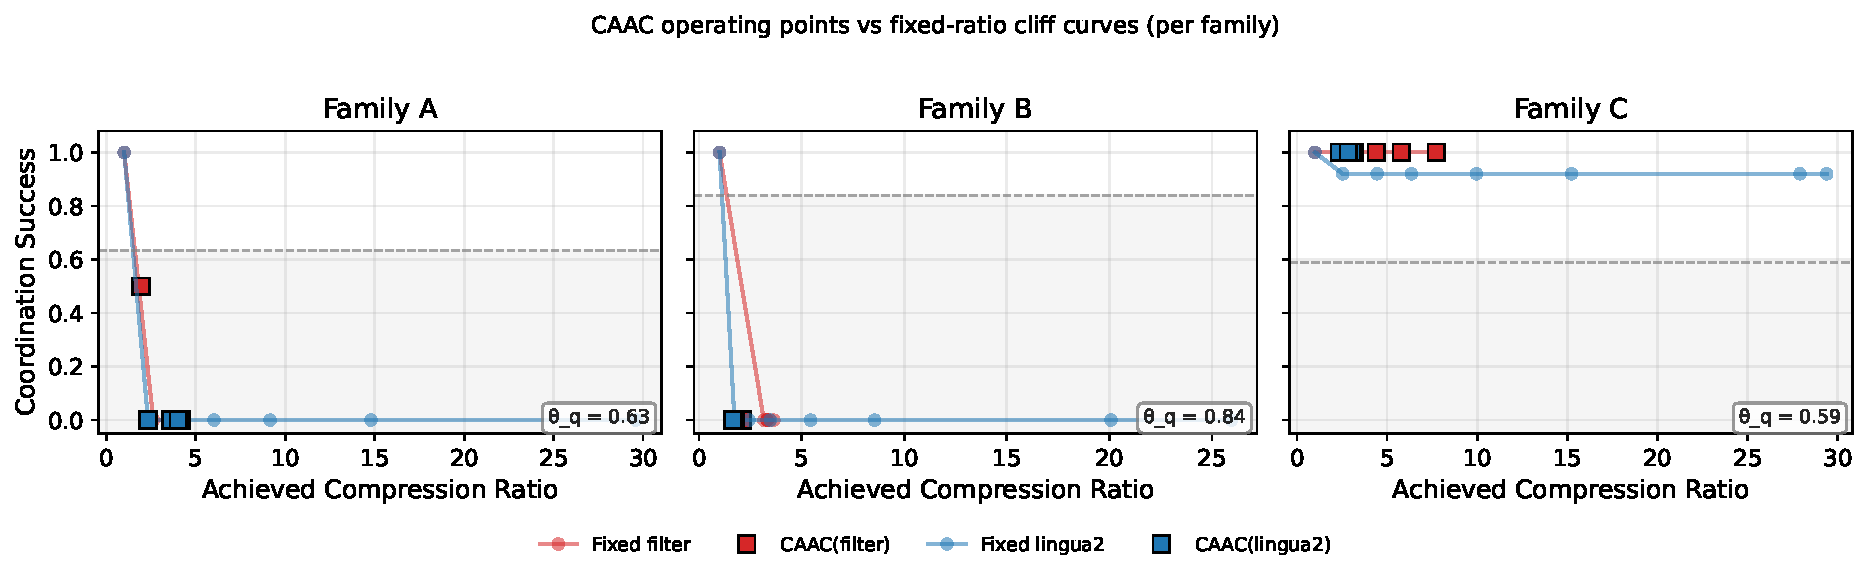
\includegraphics[width=0.74\textwidth]{../figures/caac_pareto.pdf}
\caption{CAAC and the fixed-ratio compressor on the
(coord-success, achieved-ratio) plane. The dashed horizontal line
marks the per-family $q(r) = \theta_q$ threshold from the
compounding-error model (its value annotated in each panel) and the
grey band is the sub-threshold region. CAAC's
operating points sit on the high-coord side of the threshold by
construction; the fixed compressor's points sit at the target
ratio regardless. The two compressors populate complementary
regions of the frontier; there is no strict-Pareto-dominance
relation between them.}
\label{fig:caac_pareto}
\end{figure}

\subsection{Weak-dominance result and the \texorpdfstring{$\theta_q$/$N_q$}{theta\_q/N\_q} ablation}

Although strict-Pareto does not hold, \emph{weak} dominance --- the
coordination-only comparison --- does. Across all seven target
ratios of the canonical sweep and across the two inner
compressors evaluated, CAAC's coordination success is greater
than or equal to the fixed compressor's $100\%$ of the time. At
the high target ratios where the fixed compressor cliffs to zero
coordination, CAAC retains coordination at the price of
compression. This is what the model predicts, and it is the
correct framing of CAAC's contribution: a guaranteed safety
floor, conditional on the per-family recall threshold being
correctly measured.

The $\theta_q$/$N_q$ ablation
(Section~\ref{sec:caac}; \texttt{results/caac\_theta\_*} and
\texttt{results/caac\_N\_*})
returns an informative null. Here $N_q$ is CAAC's internal
\emph{recall-exponent} knob --- the exponent in the back-off
threshold $q_\text{min}=\theta_q^{1/N_q}$ that controls how
aggressively CAAC tightens its target --- and is \emph{not} the
number of compression passes, which is fixed at one throughout
this thesis. The coordination-success plateau of
CAAC is invariant to the choice of $\theta_q$ in $\{0.6, 0.7,
0.8\}$ and the choice of $N_q$ in $\{2, 3, 4, 5\}$: the LLMLingua-2
plateau is $33\%$ across all seven configs, the filter plateau
is $50\%$ across all seven configs, and only the achieved
compression ratio responds, by backing off more aggressively as
either parameter increases. The primary knob is the
$r_\text{min}$ floor, not $\theta_q$ or $N_q$. A sweep over
$r_\text{min} \in \{1.2, 1.5, 2.0, 2.5\}$ is the natural follow-on
that this thesis defers as future work.

\subsection{What CAAC contributes to the thesis}

CAAC is the demonstration that the compounding-error model is
operationally usable, not just descriptively predictive. The
algorithm is short, training-free, drop-in, and bounded in
behaviour by a measurement. The contribution sits in
\charef{summary} rather than as a headline contribution
in \charef{introduction} because the model is the
substantive contribution and CAAC is its constructive realisation
--- but the design choice that CAAC enables is real: a
practitioner who has measured $\theta_q$ on one family can deploy
CAAC at any target ratio with the guarantee that the achieved
operating point sits on the safe side of the cliff. This
deployment-mode property is what makes the cliff measurement
useful as something other than a publication finding.

\section{Design Iteration and Methodological Course Corrections}
\label{sec:iteration}

The findings reported in \charef{experiments} are not the first
ones the empirical pipeline produced. Several measurements turned
out to be wrong on first pass and had to be regenerated; several
design choices that looked correct on paper required revision
after the first sweep made their failure modes visible. This
section surfaces those course corrections explicitly, because the
design narrative an external reviewer reads in
\charef{introduction}~Section~\ref{sec:contributions} should not
suggest that the final design fell from the sky. The catalogue is
in order of impact on the manuscript's verdict block.

\paragraph{H4 question-template bias and benchmark regeneration.}
The original H4 benchmark generator produced ``at least X''
questions whose ground-truth answer was always YES and ``exceed
X'' questions whose ground-truth was always NO. A surface-pattern
reader could in principle score $100\%$ on the verb alone. The
Llama-3.1-8B reader did not exploit this in practice (priors
stayed near $0.50$), but the data was biased, which inflated the
baseline rate to $0.97$. The generator was fixed
(\texttt{fact\_aggregation.py:119--156}) to use a single
comparator phrasing with parity-based threshold sign, the H4
sweep was rerun, and the unbiased benchmark is what every H4
number in \charef{experiments} reports. The cached
compressed-fragment data was unchanged across the rerun. Lesson:
synthetic-benchmark generators need bias audits before the reader
is held responsible for the result.

\paragraph{The \texttt{rounds} field truthfulness fix.}
An earlier version of the orchestrator reported a \texttt{rounds}
field equal to \texttt{len(sub\_tasks)}, conflating ``how many
sub-tasks did the planner see'' with ``how many rounds of agent
communication occurred''. Since the empirical setup is a single
LLM call (no multi-round communication, per
Section~\ref{sec:limitations}), the truthful value is one and the
field was changed accordingly. The earlier value never appeared in
a reported figure but was visible in some CSV columns; the
misnaming was a name-versus-meaning drift of the kind a downstream
reader could be misled by. Lesson: metric-name versus
implementation drift; metrics referenced in the manuscript text
need name-audits.

\paragraph{CAAC's \texttt{theta} hardcoded $\to$ derived.}
An initial CAAC implementation hardcoded $\theta = 0.65$ with no
derivation. The strict-Pareto rate against the fixed-ratio
compressor was $0/7$, but the verdict was ambiguous because a
different hardcoded $\theta$ would have produced a different
operating point and the model's per-family $\theta_q$ machinery
was not connected. The fix was to wire \texttt{derive\_theta()}
per-family into CAAC and reframe the strict-Pareto-zero result as
the structural property the model predicts. The $0/7$ verdict
survived the change, but is now defensible as an operating-point
property of the model rather than a tuning artefact.

\paragraph{CAAC's \texttt{min\_ratio} $1.0 \to 1.5$.}
The original CAAC implementation set \texttt{min\_ratio} to $1.0$,
which let CAAC abdicate to no-compression on hard fragments.
Pilot runs at high target ratios on family-a showed that this
abdication was the dominant CAAC behaviour, defeating the
``adaptive compression'' framing because CAAC's output on those
fragments was indistinguishable from the identity control. Raising
\texttt{min\_ratio} to $1.5$ enforces the constructive guarantee
that CAAC always delivers at least $1.5\times$ compression while
staying on the safe side of the cliff.

\paragraph{Mann--Whitney $U$ $\to$ paired Wilcoxon (mid-project).}
The first H2 cliff analyses used the Mann--Whitney $U$ test for
the two-cell drop comparison. A statistical-protocol review
(Section~\ref{sec:metric_choices} of \charef{experiments}) caught
that the same workloads appear in both conditions on the paired
comparison, which violates the independence assumption
Mann--Whitney requires. All H2 cells were recomputed under the
paired Wilcoxon signed-rank test. The verdict (cliff significant
on $11/12$ cells) was unchanged but the $p$-values tightened;
the corrected numbers are the ones in
Table~\ref{tab:h2_tau} of \charef{experiments}.

\paragraph{Fine-grid re-resolution and the canonical-reference correction.}
The early Corollary~1 evidence compared frontier-model cliffs
against a synthetic reference $\tau^{*} = 2.5$ derived from the
coarse-grid deterministic-solver sweep. A fine-grid re-resolution
that interpolated $r \in \{1.25, 1.5, 1.75\}$ between $r = 1$ and
$r = 2$ later revealed that the deterministic solver actually
cliffs at $\approx 1.1$ on family-a $\times$ LLMLingua-2; the
$2.5$ value was a grid-quantisation artefact of the coarse sweep
(\charef{experiments}~Section~\ref{sec:h2}). The Corollary~1
evidence was re-anchored to the LLM-vs-LLM comparison
(Llama-3.1-8B versus Qwen-2.5-72B both cliffing at
$\approx 2.5$--$2.8$ on the same cell), which is now the
load-bearing finding rather than the deterministic-solver number.
The cross-architecture invariance claim was strengthened rather
than weakened by the correction; the early framing against
$\tau^{*} = 2.5$ is retained only as an approximate coincidence
between the LLM cliff and the coarse-grid deterministic value.
Lesson: always run a fine-grid re-resolution at the cliff midpoint
before publishing position numbers.

\paragraph{$\theta_\text{info}$ estimator unification.}
An earlier value for C1 family-a's $\theta_\text{info}$ was
$0.881$, computed by a different estimator from the current
AUC-based \texttt{estimate\_task\_theta()} implementation. After
the estimator was unified across the three benchmarks the
canonical value is $0.967$ (Table~\ref{tab:corollary2} of
\charef{experiments}). The corollary verdict and the
dense-vs-distributed ordering were unchanged; the absolute number
shifted by $\sim 9\%$ because of the estimator change. Lesson:
cross-benchmark estimates require a single estimator
implementation reused across benchmarks.

\paragraph{Theorem~1 $\to$ compounding-error model.}
The early draft of \charef{experiments} called
Section~\ref{sec:cem} ``Theorem~1'' and shipped a formal LaTeX
proof. The empirical match rate ($33\%$ at $\pm 25\%$) is the
wrong character for a ``theorem'', because the residuals are
dominated by specification error rather than sampling error. The
naming was downgraded to ``compounding-error model'' and the
formal proof was dropped; the derivation paragraph is what
survives in Section~\ref{sec:cem}. Codebase identifiers
(\texttt{theorem\_validation.json},
\texttt{validate\_theorem.py}) are retained for backwards
compatibility with on-disk artefacts and are documented in the
project repository.

The aggregate lesson across these corrections is that a verdict
pipeline whose intermediate outputs are spot-checked against
expected shapes catches errors that a single end-to-end run does
not. The compression cache
(\charef{implementation}~Section~\ref{sec:cache}) supports this by
making intermediate outputs persistent and inspectable; the
practice generalises to any thesis whose experiment pipeline
iterates many times over the same workloads.

\section{Limitations}
\label{sec:limitations}

The limitations are catalogued explicitly so that a reader can
calibrate the scope of the findings.

\paragraph{No multi-round agent coordination.}
The empirical evaluation uses a deterministic regex solver
(H1, H2) or a single LLM call with all (compressed) fragments
visible (Corollary~1, frontier, real-data transfer). The AutoGen
v0.4 multi-round agent backend in
\texttt{src/m6/orchestrator/} integrates with the memory bus but
is not used in any reported result. Multi-round coordination
introduces a per-round variance that the deterministic solver
deliberately excludes; the cliff measured here is the
solvability cliff under compression, not the multi-round
communication-quality cliff. This scoping decision is recorded in the project repository.

\paragraph{Single compression pass.}
Every experiment uses $N=1$. The compounding-error model admits
arbitrary $N$ ($q$ compounds as $q^N$), but the $N>1$ regime is
not empirically validated. The $\theta_q$/$N_q$ ablation
(Section~\ref{sec:caac}) is an algorithmic sweep over CAAC's
internal recall-exponent knob $N_q$, not a sweep of the number of
compression passes (which stays fixed at one). Multi-pass coordination is a natural follow-on
study.

\paragraph{Family-a homogeneity.}
The $50$ instances of family-a are all sum-of-eight-numbers
variants. The cliff structure observed on family-a may not
generalise to heterogeneous aggregation tasks (max, min, weighted
average, conditional aggregation). The transfer to real benchmarks
(Corollary~2) addresses the broader concern that synthetic tasks
might not transfer to real ones, but the within-family
homogeneity is a separate concern that future work could resolve
by sweeping aggregation types within family-a.

\paragraph{Family-b LLM floor.}
The constraint-satisfaction family-b is hard for $\le 8$B planners
independent of compression: baseline coordination success is near
zero for the $1.5$B (Qwen-2.5) and $3.8$B (Phi-3-Mini) planners.
The family-b cliff is
not detectable in this regime, and Corollary~1's invariance
result is therefore tested on family-c only for the local sweep.
A planner capable of solving family-b at the no-compression
baseline (e.g., a frontier reasoning model) would enable a
family-b validation of Corollary~1 that this thesis cannot
produce.

\paragraph{Phi-3-Mini extractive ceiling.}
The Phi-3-Mini extractive compressor saturates at approximately
$2.5\times$ achievable compression regardless of the requested
target, because the verifier and the LLMLingua-2 fallback combine
to bound the achievable ratio. All evaluation reports the
achieved ratio alongside the requested target so this saturation
is visible, but it does mean that Phi-3-Mini extractive cannot
participate in the high-compression-ratio comparisons; its curves
flatten above $\sim 2.5\times$ rather than continuing to follow
the family's degradation pattern.

\paragraph{Extended-reasoning regime is out of scope.}
The calibrated regime predicate (Section~\ref{sec:calibrated})
excludes planners that recover sub-threshold information by
chain-of-thought reasoning. GPT-oss~120B and likely the GPT-4-class
``thinking'' models violate the predicate. The
compounding-error model's quantitative predictions do not apply
to these planners; the GPT-oss~120B result is reported as an
out-of-regime diagnostic in Section~\ref{sec:frontier} rather
than as a counterexample. Characterising the cliff in the
extended-reasoning regime is the largest follow-on direction this
thesis opens.

\paragraph{Compounding-error model is a first-order bound.}
The predicted-versus-empirical $\tau^{*}$ match is first-order, not
tight (median $35.3\%$ relative error; full match rates in
Section~\ref{sec:cem_match}). The model is useful as a first-order
predictor and as a derivation that explains the cliff's sharpness,
not as a precise prediction. Its graded-importance assumption~A2 is
the strongest of the four (Section~\ref{sec:cem_assumptions}), and
H4's graded-disclosure measurements are evidence for exactly the
binary-importance simplification the model gives up.

\paragraph{Predicted-$\tau^{*}$ bootstrap band is too tight.}
The bootstrap CI on $\theta_q$ behind the
Section~\ref{sec:cem_match} band quantifies \emph{sampling}
uncertainty only, not the model's \emph{specification} error, so the
empirical $\tau^{*}$ falls outside it on all $11$ testable cells.
Figure~\ref{fig:predicted_vs_empirical} should be read as ``the band
is tight because $\theta_q$ is well-estimated; the model is biased
because A1--A4 are first-order'' --- the in-sample/LOO match rates,
not the band, measure the model's accuracy.

\paragraph{Corollary~1's local arm misses the strict tolerance.}
The local cross-architecture sweep (Qwen-2.5-1.5B, Phi-3-Mini-3.8B,
Llama-3.1-8B) on family-c shows a $\tau^{*}$ spread of $\approx 24\%$
--- below the \texttt{validate\_model\_independence} default $50\%$
tolerance but above the strict $\pm 20\%$ bar matching the H2 spec.
The local arm is thus necessary but not sufficient; the
cross-architecture frontier evidence (Section~\ref{sec:frontier})
carries the corollary's binary verdict across the strict bar
(\texttt{results/h5\_final/model\_independence\_20pct.json}).

\paragraph{A3 (threshold success): circularity broken by a direct probe.}
A3 was originally licensed only by the sharp cliff it explains --- a
circular justification --- now broken by the independent A3 probe
(Section~\ref{sec:a3_probe}, \texttt{results/a3\_probe}): curated
deletion of task-critical tokens \emph{without} a compressor, scored
by an LLM planner that \emph{could} reconstruct partial information.
It supports A3 directly on the dense aggregation family
(threshold-like, $k\approx 15$) and shows it is only first-order on
the distributed family (graded, $k\approx 5.9$). The honest residual
statement is that A3 is a threshold model for dense tasks and a
first-order approximation for distributed ones --- the same
information-density axis Corollary~2 measures --- with a
graded-success refinement as the open direction. The cliff exists
regardless; A3 describes its shape.

\paragraph{A1 within-pass independence is approximate;
Phi-3 extractive violates it.}
A1 (per-token retention independent across positions) holds
approximately for token-level compressors (LLMLingua-2,
instruction-aware filter, truncation baseline). It is violated by
Phi-3-Mini extractive, which selects whole spans, inducing
correlated token-survival events within a span. The
phi3-extractive validation cells in Section~\ref{sec:cem_match}
should be read as a robustness check of the bound \emph{outside}
its formal A1 regime rather than as a within-regime prediction.

\paragraph{Synthetic-task focus, real-task transfer at the
structural level.}
The C1 benchmark is synthetic, by design: cliff characterisation
requires controlled information density. The transfer validation
on HotpotQA and MultiHop-RAG shows that the cliff structure
(existence, sharpness gradient with $\theta_\text{info}$) transfers
to real benchmarks, but the absolute cliff positions differ
substantially. Generalisation to arbitrary task structures
beyond the three task families this thesis examines is unverified
and would require either a broader benchmark suite or a
\texttt{theta\_info} sweep over a corpus of real benchmarks.

\paragraph{Single-retriever, single-embedder RAG comparison.}
The H3 RAG pipeline catalogue uses FAISS-CPU with HNSW and
\texttt{BAAI/bge-large-en-v1.5} embeddings. Different retrievers
or embedders may shift the cost balance of the storage- and
accuracy-bounded regimes. The compress-first-over-retrieve-first
finding is qualitatively robust, since it depends on the
storage-cost asymmetry, which holds for any retriever. It is
nonetheless demonstrated on only this one stack, so we report it as
a single-stack non-reproduction of the LongLLMLingua preference
rather than a general falsification.

\paragraph{H3 cost model is corpus-dominated and does not meter
compression.}
The \texttt{eur\_per\_query} ledger is corpus-dominated --- the
three pipelines differ by only $4.1$--$4.9\%$ within a regime --- and
does not meter compression \emph{compute} at all
(Section~\ref{sec:h3_cost_caveat}). The cost-instrumented re-run
shows P2/P3 route fragments verbatim (achieved ratio $1.00\times$)
while only P1 compresses, so the cross-pipeline F1 comparison is not
matched on compression and the thesis makes no cost-parity or Pareto
claim for P3-vs-P1. A faithful per-pipeline cost model is required to
attribute P3's F1 advantage to routing rather than to uncharged cost
(Section~\ref{sec:future}).

\paragraph{Frontier equivalence not established (underpowered).}
A percentile-bootstrap TOST against the $\pm 20\%$ equivalence band
(Section~\ref{sec:frontier_deepseek};
\texttt{results/tost\_corollary1.json}) shows \emph{neither}
frontier cell passes: although the point estimates match the
reference well (Qwen-2.5-72B $\sim 7\%$ from the canonical
$\tau^{*}=2.5$, within $0.8\%$ of the auxiliary fit $2.6997$), the
$90\%$ bootstrap intervals on $\tau^{*}$ are too wide to rule out a
$>20\%$ difference. Corollary~1's frontier evidence is therefore
correctly stated as ``no cliff-position shift detected'' rather than
``invariance demonstrated''; tightening it to a passed equivalence
test requires more seeds per frontier cell (future work).

\paragraph{Reader-bias in H4 measurement.}
The Llama-3.1-8B reader under-predicts YES protected-fact
answers. The pooled rates that the H4 verdict rests on are
balanced by the ground-truth class distribution rather than by
reader-side accuracy. The H4 metric measures
\emph{``compression preserves enough information to flip a
no-biased reader to confident YES''}, which is an asymmetric
leakage signal. A reader chosen specifically to be unbiased
would distinguish the disclosure-reduction signal from the
reader's prior; this is named as future work in
Section~\ref{sec:future}.

\section{Significance}
\label{sec:significance}

\subsection{For practitioners}

Four practitioner-facing implications follow from the findings.

First, single-agent question-answering benchmarks (LongBench,
RULER, the LLMLingua line of work's own QA evaluations)
\emph{systematically over-report} compressor utility for
multi-fragment deployments. A multi-fragment evaluation is
necessary; this thesis ships one (C1) and a methodology
(the cliff sweep) that other groups can apply on their own
workloads.

Second, the cliff position can be predicted from per-round token
recall plus a one-shot $\theta_q$ measurement, within a known
first-order tolerance. A practitioner who needs to choose a
compression ratio for a new multi-fragment workflow can run the
$\theta_q$ measurement on a small calibration set and apply the
compounding-error model to obtain a safe operating point without
running the full cliff sweep.

Third, compress-first (P1) is the better RAG architecture between
the two compressed-corpus pipelines in both regimes \emph{on the
single retriever/embedder stack tested} (a result that does not
reproduce the LongLLMLingua post-retrieval-compression preference
on this stack, but is not a general falsification). Joint
relevance-conditional routing (P3) scores higher F1 still
($42$~pp storage, $25$~pp accuracy). That advantage, however, comes
from \emph{not compressing}: Section~\ref{sec:h3} shows P3 routes
fragments verbatim (achieved ratio $1.00\times$), and the
corpus-dominated cost model does not meter the compressor pass. The
F1 ranking $\mathrm{P3} \succ \mathrm{P1} \succ \mathrm{P2}$ is
therefore reported \emph{without} a cost-parity claim; whether P3's
quality gain is cost-free is undetermined until the per-pipeline
cost model is fixed. The defensible practitioner takeaway is narrower than a
clean ranking: on this stack, prefer compress-first over
retrieve-first, and treat P3 as a promising routing variant whose
cost must be measured before deployment.

Fourth, compression is a privacy lever --- but a \emph{blunt}
one, and the bluntness creates a policy conflict the memory bus
does not yet resolve. The disclosure metric ranks compressors by
leakage at iso-ratio, so a governance budget on protected-fact
leakage can be enforced by routing \textsc{confidential} fragments
through the compressor (and ratio) whose disclosure rate meets the
budget. The conflict is this: Section~\ref{sec:h4_disclosure}
shows the privacy gain is \emph{destruction-driven} --- leakage
falls because tokens are destroyed --- which is the
\textbf{same lever}, pointed the other way, that the coordination
cliff warns against. For a fragment that is simultaneously
privacy-sensitive and coordination-critical, ``compress more to
leak less'' and ``compress less to stay above $\tau^{*}$'' are
directly opposed, and the disclosure-reduction and coordination-loss
are not independent axes but two readings of one quantity
(information destroyed). The reference bus exposes both signals
(disclosure rate and CTR) but provides \textbf{no arbitration
rule} for fragments where they conflict; choosing an operating
point that satisfies a leakage budget \emph{and} a coordination
floor --- when both are feasible at all --- is named as future
work (Section~\ref{sec:future}). Practitioners should treat the
privacy lever as usable only for fragments that are \emph{not} on
the coordination-critical path, until such an arbitration policy
exists.

\subsection{For the field}

Three field-facing claims are substantive.

First, the cliff is a property of the (compressor, task) pair and
of the planner \emph{class}, not of planner scale or architecture
within a class: the LLM-planner cliff on family-a $\times$
LLMLingua-2 is essentially invariant across a $9\times$ scale-up and
a change of architecture family, well above the brittle
deterministic-solver cliff on the same cell. The implication for the
compression literature is that future compressor evaluations should
either characterise the calibrated regime they apply in or
explicitly target the extended-reasoning regime as a separate case.

Second, extended-reasoning planners are a different regime that
the existing compression literature has not characterised. The
GPT-oss~120B out-of-regime result is a positive diagnostic of
where the threshold-success assumption breaks; characterising
this regime systematically is a publishable follow-on. The
practical-deployment implication is that compression ratios
calibrated on a non-reasoning planner cannot be transferred to a
reasoning planner without revalidation.

Third, information density $\theta_\text{info}$ scales the cliff
across benchmarks in a way that future benchmarks should
control for. A multi-benchmark compression-quality comparison
that does not measure or control $\theta_\text{info}$ will report
cliff positions that conflate compressor mechanism with task
structure; the cross-benchmark transfer result of Corollary~2 is
the evidence that the two must be separated.

\section{Comparison to Industry Observations}
\label{sec:industry_comparison}

The closest published industry observation --- Anthropic's report
that token usage explains $\approx 80\%$ of the performance variance
in their multi-agent research workflow~\cite{anthropic2025multiagent},
with the follow-on context-engineering and context-editing
reports~\cite{anthropic2025contextengineering, anthropic2025contextediting}
--- is consistent with this thesis and underwrites the practitioner
urgency. What it does not provide, and what the thesis contributes,
is the structural characterisation: the Anthropic report is an
aggregate observation on a single workflow, whereas the cliff
measurement here is a controlled cross-compressor, cross-family,
cross-architecture sweep with a model that predicts the cliff
position. The industry observation is the macro reason a practitioner
cares; the thesis findings are the micro answer that lets them act.

\section{Future Work}
\label{sec:future}

The most natural follow-on studies in order of expected impact.

\paragraph{Extended-reasoning regime.}
Characterise the cliff for planners that recover from
sub-threshold information by chain-of-thought reasoning. The
empirical setup is a re-run of the cliff sweep with
GPT-oss-class planners, GPT-4-Turbo with thinking, and Claude
Sonnet 4.6 with extended thinking enabled. The theoretical work
is replacing A3 (threshold success) with a graded-success model.

\paragraph{Graded-success refinement of the A3 model.}
The direct A3 probe (now in the results chapter,
Section~\ref{sec:a3_probe}) confirms the threshold mechanism on
the dense aggregation family but shows a clearly \emph{graded}
success curve on the distributed retrieval family
($k\approx 5.9$, transition band $\approx 0.54$ wide). The remaining
open theoretical direction is therefore a graded-success refinement
of A3 that recovers the threshold form as the
information-density-high limit. The same axis also underlies
Corollary 2's $\theta_\text{info}$ scaling (dense $\Rightarrow$
threshold, distributed $\Rightarrow$ graded), so the refinement
is the natural common ancestor of A3 and Corollary 2.

\paragraph{Per-task $\theta_q$ estimation.}
Lift the model from per-family $\theta_q$ to per-task
$\theta_q$. The current per-family validation match rate is
$33\%$ strict in-sample ($25\%$ under leave-one-family-out
cross-validation; see Section~\ref{sec:cem_match} for the gap);
a per-task fit should improve this to the $60$--$70\%$ range
observed on the $\theta_q$-already-known calibration cells,
against the LOO baseline rather than the in-sample one. The
empirical setup is straightforward; the methodological cost is
fitting $\theta_q$ per task on a held-out calibration split.

\paragraph{Multi-pass compression at $N > 1$.}
Validate the $q^N$ formulation of the model empirically. The
empirical setup is a small sweep across two-pass and three-pass
compression on the family-a cells; the analysis turns on whether
the empirical cliff shifts predictably with $N$.

\paragraph{CAAC $r_\text{min}$ sweep.}
The $\theta_q$/$N_q$ ablation showed that the CAAC operating-point
plateau is invariant to those two parameters. The primary knob
the ablation deferred is $r_\text{min}$. A sweep over
$r_\text{min} \in \{1.2, 1.5, 2.0, 2.5\}$ produces the
operating-point family that CAAC traces out as a function of the
floor.

\paragraph{Multi-round AutoGen coordination.}
The AutoGen v0.4 multi-round backend is wired into the memory
bus but excluded from the empirical evaluation because of
run-to-run variance. A focused study that controls the
round-count variance and isolates the per-round compression
effect would extend the thesis findings to the multi-round
coordination regime that the deterministic-solver scope of this
thesis deliberately defers.

\paragraph{Faithful per-pipeline RAG cost model.}
The H3 ledger is corpus-dominated and does not meter compression
\emph{compute} (Section~\ref{sec:h3_cost_caveat}), which prevents
any cost-parity claim. A corrected model would meter each pipeline's
token economics separately, amortise a persistent index rather than
re-charge the corpus each query, and re-evaluate P3-vs-P1 on a
binding storage constraint --- only then can P3's F1 lead be
attributed to routing rather than to an unmetered cost.

\paragraph{Frontier equivalence: more seeds to tighten the CI.}
Neither frontier cell passes $\pm 20\%$ TOST equivalence
(Section~\ref{sec:frontier_deepseek}), so the defensible claim is
``no shift detected'', not ``equivalent''. Increasing the per-cell
frontier sample would stabilise the piecewise fit under resampling
--- the DeepSeek bootstrap median $5.7$ sitting far from its point
estimate $2.15$ signals the instability --- and could convert ``no
shift detected'' into a passed equivalence test (or refute it).

\paragraph{Memory-bus systems benchmark.}
C4's single-threaded core operations are characterised on two hosts
with sub-millisecond tail latency (Section~\ref{sec:bus_bench}). The
benchmark uses the identity compressor and the in-process SQLite
audit log, so the upgrade from ``characterised single-threaded'' to
``production characterised'' is a concurrent-HTTP-path throughput
sweep and an audit-verify scaling curve across chain lengths.

\paragraph{Standalone dissemination of the H1 result.}
The H1 finding --- that single-fragment information preservation
does not transferably predict multi-fragment coordination success,
so the single-agent QA benchmarks dominating the compression literature mis-rank
compressors for multi-fragment use --- is the most citable
standalone contribution and is independent of the model and the bus.
A focused workshop paper built around H1 (the per-family Spearman
decomposition plus the cliff existence result) is the lowest-friction
route to external validation of the thesis's central methodological
claim.

\paragraph{Broader task families.}
The three C1 families are deliberate probes of a single property
each (density, constraint-tracking, chain-reference). A broader
benchmark suite with heterogeneous aggregation types, multi-tool
reasoning, and multimodal fragments would test the
generalisability of the cliff structure beyond the families this
thesis evaluates.

\paragraph{An unbiased H4 reader --- partially addressed by class re-weighting.}
Class re-weighting (the cheaper option) was already applied: the
disclosure-reduction conclusion is \textbf{robust} to it ---
class-balanced reductions are within a percentage point of the
pooled values and the destruction-monotonic ordering is unchanged,
downgrading the Section~\ref{sec:h4_bias} caveat from ``the verdict
may rest on a reader artefact'' to ``the verdict survives
class-balancing.'' The remaining open item is larger-reader
confirmation (e.g.\ Llama-3.3-70B), expected to be confirmatory.

\section{Closing}

The five empirical findings, the compounding-error model that
ties them together, the memory-bus reference implementation
that operationalises the privacy lever, and the CAAC algorithm
that operationalises the cliff bound, jointly constitute the
thesis's contribution: a structural characterisation of context
compression in multi-fragment LLM workflows, measured across
compressors, families, and benchmarks --- with planner-scale and
architecture invariance reported as no-shift-detected rather than
established --- supported by a first-order position model, a
deployment artefact, and a reproducibility package. The single deliverable
sentence is the thesis's refrain: every token that
does not change the answer is waste, and what this thesis
contributes is a way of knowing which tokens those are, when
removing them is safe, and what the cost is when removing them
is not.


\printbibliography[heading=bibnumbered, title=\mybibname]

\startappendix
\chapter{Appendices}
  \label{appendix}
  % Appendix chapter — populated with thesis-relevant material.

\noindent The appendices collect four artefacts that support the main
text but would interrupt its narrative: the memory-bus HTTP contract
(Appendix~A), the canonical long-format results-dataframe schema used by
every experiment runner (Appendix~B), an example C1 workload
instance from family~(a) showing the source-fragment structure
(Appendix~C), and a one-command reproducibility recipe together with
an illustrative \texttt{curl} trace (with timestamps and chain hashes
elided for legibility) exercising the memory-bus endpoints
(Appendix~D). The full reproducibility package, including the
model cards and the data cards, is shipped with the reference
release referenced in the closing section of
\charef{summary}.

\section{Appendix A. Memory-Bus HTTP Contract}
\markboth{left}{\normalfont{Appendix A. Memory-Bus HTTP Contract}}

The reference memory-bus service exposes four endpoints. The contract
below summarises the request and response shapes; the authoritative
OpenAPI schema lives at \texttt{docs/openapi.json} in the repository
and is regenerated via \texttt{make bus-openapi}.

\begin{description}\setlength\itemsep{0pt}
\item[\texttt{POST /v1/write}] Body: a \texttt{Fragment} JSON object
(\texttt{fragment\_id}, \texttt{text}, \texttt{tags}) and an optional
\texttt{target\_ratio}. Returns the assigned \texttt{slot\_id}, the
audit row identifier, and the hex-encoded \texttt{chain\_hash}.
HTTP $201$ on success; $403$ on policy denial.

\item[\texttt{GET /v1/read/\{slot\_id\}}] Returns a
\texttt{CompressedSlot} with its payload, tags, compressor identifier,
nominal ratio, and creation timestamp. HTTP $200$ on success;
$403$ on policy denial; $404$ on slot not found.

\item[\texttt{POST /v1/subscribe}] Body: a \texttt{SubscribeRequest}
with a \texttt{query} string, a \texttt{ttl\_seconds} positive integer,
and a top-\textit{k} integer. Returns a server-sent-event stream
emitting newly matched \texttt{slot\_id}s with their cosine scores
until the TTL elapses.

\item[\texttt{GET /v1/audit/\{slot\_id\}}] Returns the chronological
list of \texttt{AuditRow} entries that mention the given slot.
\end{description}

Every request is processed by the \texttt{PolicyMiddleware}, which
parses the requester principal from the \texttt{X-M6-Principal} header
in the development build and from an OAuth/JWT verifier in a production
deployment. The principal carries a $64$-bit access-control mask and a
$5$-tier classification level (PUBLIC $<$ INTERNAL $<$ CONFIDENTIAL $<$
RESTRICTED $<$ SECRET). A request is granted access to a slot when the
principal's mask is a superset of the slot tag's mask and the
principal's classification is at least the slot tag's classification.

\section{Appendix B. Long-Format Results Schema}
\markboth{left}{\normalfont{Appendix B. Long-Format Results Schema}}

Every experiment runner writes its results to a CSV that conforms to
the long-format schema implemented as
\texttt{m6.evaluation.statistics.LongDF}. The columns are listed in
Table~\ref{tab:longdf}.

\begin{table}[h]
\centering
\caption{The canonical long-format dataframe schema used by every
experiment runner. The same schema underlies every CSV under
\texttt{results/}, which makes cross-hypothesis analysis a single
\texttt{pandas.concat} away.}
\label{tab:longdf}
\small
\begin{tabular}{p{4cm}p{2.5cm}p{6.5cm}}
\hline
Column & Type & Notes \\
\hline
\texttt{experiment\_id} & str & unique per run \\
\texttt{hypothesis} & str & one of \texttt{h1}\,\ldots\,\texttt{h6} or \texttt{caac}, \texttt{frontier}, \texttt{hotpotqa} \\
\texttt{compressor} & str & e.g.\ \texttt{lingua2}, \texttt{filter},
\texttt{phi3-extractive}, \texttt{truncation}, \texttt{caac}, \texttt{identity} \\
\texttt{ratio} & float & nominal compression ratio \\
\texttt{actual\_ratio} & float & measured ratio post-compression \\
\texttt{pipeline} & str & one of \texttt{none}, \texttt{P1},
\texttt{P2}, \texttt{P3} \\
\texttt{model} & str & e.g.\ \texttt{llama-3.1-8b-instruct} \\
\texttt{model\_size} & str & \texttt{1.5b}, \texttt{3.8b}, \texttt{8b}, \texttt{72b} \\
\texttt{workload\_family} & str & \texttt{a}, \texttt{b}, or \texttt{c} \\
\texttt{workload\_id} & str & e.g.\ \texttt{c1-a-007} \\
\texttt{seed} & int &  \\
\texttt{metric} & str & e.g.\ \texttt{coord\_success}, \texttt{qa\_f1},
\texttt{preservation\_rate} \\
\texttt{value} & float &  \\
\texttt{wallclock\_ms} & int &  \\
\texttt{eur\_cost} & float &  \\
\texttt{run\_id} & str &  \\
\texttt{git\_sha} & str &  \\
\texttt{config\_hash} & str &  \\
\texttt{created\_at} & str & ISO-8601 UTC \\
\texttt{invalid} & bool & control-condition variance dominates? \\
\texttt{invalid\_reason} & str & free-text explanation if invalid \\
\hline
\end{tabular}
\end{table}

\section{Appendix C. Example C1 Workload (family a)}
\markboth{left}{\normalfont{Appendix C. Example C1 Workload}}

The following JSON object illustrates a single instance of C1
family~(a) (cross-document fact aggregation). Each fragment represents
one institutional system; the planner is asked to aggregate hours and
budget across all eight; the critic verifies the answer against the
ground-truth aggregate.

\begin{verbatim}
{
  "workload_id": "c1-a-007",
  "family": "a",
  "seed": 1247,
  "tag_distribution": "skewed",
  "initial_prompt":
    "Aggregate the period-end report for project P-0001 across the
     following systems: system_1, system_2, system_3, system_4,
     system_5, system_6, system_7, system_8. Report total hours and total
     budget.",
  "expected_answer": "hours=853;budget=148340",
  "n_agents": 8,
  "fragments": [
    {
      "fragment_id": "c1-a-007/system_1",
      "text": "[system_1] Project P-0001 - period 2025-Q3. ...",
      "tags": {"acl_mask": 12876, "classification": 1}
    },
    {
      "fragment_id": "c1-a-007/system_2",
      "text": "[system_2] Project P-0001 - period 2025-Q3. ...",
      "tags": {"acl_mask": 8901, "classification": 2}
    }
    // (six more fragments, one per system)
  ],
  "sub_tasks": [
    {
      "sub_task_id": "c1-a-007/sub-0",
      "description":
        "Extract recorded hours and budget for project P-0001 from
         system_1.",
      "expected_solver": "worker-0",
      "expected_answer": "hours=112;budget=18420"
    }
    // (seven more sub-tasks)
  ],
  "protected_facts": [
    {
      "fragment_id": "c1-a-007/system_2",
      "fact": "system_2.budget=22150",
      "yesno_questions": [
        "Did system_2 for project P-0001 exceed EUR 27150 in budget?",
        "Was system_2's recorded hours for P-0001 more than 142?"
      ],
      "answers": ["no", "no"]
    }
  ]
}
\end{verbatim}

The full dataset is reproduced from
\texttt{configs/benchmark/c1-v0.1.yaml} via \texttt{make
bench-generate}; the manifest carries the configuration hash so any
reader can verify they are looking at the same release.

\section{Appendix D. Reproducibility Recipe and Memory-Bus Trace}
\markboth{left}{\normalfont{Appendix D. Reproducibility Recipe and Memory-Bus Trace}}

\subsection{D.1 One-command reproduction of every chapter figure}

The reproducibility package is the complete reference repository
released to examiners and collaborators.
Historical planning documents in the repository reflect earlier
protocol designs; the canonical experiment protocol for the submitted
thesis is the final set of experiment runners and result artefacts
listed here.
The package contains a \texttt{docker-compose.yml} that
brings the memory-bus reference service up locally, a GitHub
release tag matched to the manuscript, model and data cards under
\texttt{docs/}, and a \texttt{README.md} that exposes
one-command reproduction targets for every headline figure (the
compute envelope and software stack are detailed in
Section~D.3):

\begin{description}\setlength\itemsep{1pt}
\item[\texttt{make repro-bench}]
regenerates the $150$-instance C1 benchmark from
\texttt{configs/benchmark/c1-v0.1.yaml}. Output:
\texttt{data/processed/c1-v0.1/}.
\item[\texttt{make repro-cache}]
runs the compression precomputation for all four compressors at
the ten canonical ratios across the $150$ workloads. Requires
the GPU host; total wallclock $\sim 14$~hours. Output:
\texttt{results/compression\_cache/}.
\item[\texttt{make repro-cliff}]
runs the H1/H2 cliff sweep against the compression cache,
producing all of \charef{experiments}'s Section~\ref{sec:h1}
through Section~\ref{sec:cem_match} figures. Wallclock
$\sim 3$~hours on the M4~Pro.
\item[\texttt{make repro-scaling}]
runs the model-scaling sweep at $1.5$B, $3.8$B, and $8$B with the
local Ollama backend, producing Corollary~1's figures. Wallclock
$\sim 90$~minutes.
\item[\texttt{make repro-frontier}]
runs the cliff sweep against the Featherless API for
Qwen-2.5-72B-Instruct and DeepSeek~V4~Pro, the two
calibrated-regime frontier validators. (The out-of-regime
GPT-oss-120B diagnostic is scoped out of the canonical recipe as
an extended-reasoning planner and is not part of this target.) Requires a
\texttt{FEATHERLESS\_API\_KEY}. Output:
\texttt{results/frontier\_\{qwen72b,deepseekv4\}/}.
\item[\texttt{make repro-rag}]
runs the H3 RAG pipeline catalogue, producing
Section~\ref{sec:h3}'s figures. Wallclock $\sim 3$~hours.
\item[\texttt{make repro-disclosure}]
runs the H4 inference-disclosure measurement against the unbiased
benchmark, producing Section~\ref{sec:h4_disclosure}'s figures.
Wallclock $\sim 1$~hour on the M4~Pro.
\item[\texttt{make repro-transfer}]
runs the HotpotQA and MultiHop-RAG transfer arm, producing
Section~\ref{sec:corollary2}'s figures. Wallclock $\sim 2$~hours.
\item[\texttt{make repro-figs}]
regenerates every PDF and PNG figure under \texttt{figures/} from
the canonical CSVs. Pure-Python; runs in under a minute.
\end{description}

The \texttt{make repro-all} target chains the six laptop-runnable
steps above (\texttt{repro-cliff}, \texttt{repro-scaling},
\texttt{repro-rag}, \texttt{repro-disclosure},
\texttt{repro-transfer}, and \texttt{repro-figs}) in dependency
order, excluding the two that need special resources:
\texttt{repro-cache} (GPU host) and \texttt{repro-frontier} (a
Featherless API key), which must be run explicitly; the whole
package is $\sim 30$~hours of GPU time and $\sim 12$~hours of laptop
time end-to-end. The byte-deterministic / in-distribution /
not-reproducible status of each target follows the three-tier
guarantee of Section~\ref{sec:repro} (\charef{experiments}):
\texttt{repro-cache}, \texttt{-cliff}, \texttt{-rag},
\texttt{-disclosure}, and \texttt{-figs} are Tier~1,
\texttt{repro-scaling} is Tier~2, and \texttt{repro-frontier} is
Tier~3.

\subsection{D.2 Memory-bus end-to-end trace}

The following \texttt{curl} sequence exercises the four
endpoints of the memory bus end-to-end against the
\texttt{docker-compose}-up'ed reference service. The trace is
the rubric-\#5 evidence for the C4 contribution: the memory bus
is a running system, not a paper design. The output of each step
is reproduced from a run against the reference image
tagged \texttt{m6-memory-bus:thesis-v1.0}, with timestamps and chain
hashes elided for legibility.

\begin{verbatim}
# Step 1: Write a CONFIDENTIAL fragment with target ratio 4x.
$ curl -X POST http://localhost:8000/v1/write \
       -H "Content-Type: application/json" \
       -H "X-M6-Principal: principal=alice;acl=0xFFFF;cls=3" \
       -d @- <<'EOF'
{
  "fragment_id": "demo-001",
  "text": "Project P-0001 quarterly hours: 112; budget: EUR 18420.",
  "tags": {"acl_mask": 12876, "classification": 2},
  "target_ratio": 4.0,
  "compressor": "lingua2"
}
EOF
{"slot_id": "slot-1a4b9c2d", "audit_row": 1,
 "chain_hash": "5f3d2a1b...",  "achieved_ratio": 3.72}

# Step 2: Read the slot back. The principal's classification (3)
#         is at least the slot's (2) and the principal's ACL mask
#         is a superset, so the read is permitted.
$ curl -H "X-M6-Principal: principal=alice;acl=0xFFFF;cls=3" \
       http://localhost:8000/v1/read/slot-1a4b9c2d
{"slot_id": "slot-1a4b9c2d",
 "compressed_text": "Project P-0001 hours: 112 budget: 18420.",
 "compressor": "lingua2", "achieved_ratio": 3.72,
 "tags": {"acl_mask": 12876, "classification": 2},
 "created_at": "2026-05-30T07:42:15Z"}

# Step 3: A second principal with insufficient classification is
#         denied; the denial is itself audited with a
#         per-(principal, slot) 60-second deduplication.
$ curl -H "X-M6-Principal: principal=bob;acl=0xFFFF;cls=1" \
       -o /dev/null -w "%{http_code}\n" \
       http://localhost:8000/v1/read/slot-1a4b9c2d
403

# Step 4: Audit walk for the slot. The chain is verifiable end-to-
#         end via the SHA-256 chain hash on each row; tampering
#         with any row breaks verification.
$ curl -H "X-M6-Principal: principal=alice;acl=0xFFFF;cls=3" \
       http://localhost:8000/v1/audit/slot-1a4b9c2d
[
  {"rowid": 1, "event_type": "WRITE",  "result": "OK",
   "requester": "alice", "chain_hash": "5f3d2a1b..."},
  {"rowid": 2, "event_type": "READ",   "result": "OK",
   "requester": "alice", "chain_hash": "9c4e7a8d..."},
  {"rowid": 3, "event_type": "READ",   "result": "DENIED",
   "requester": "bob",   "chain_hash": "1b8a6f3e..."}
]
\end{verbatim}

The trace illustrates four properties: compression with achieved-
ratio reporting on the write path; policy-checked read with the
five-tier classification lattice and the access-control mask;
audited denial with the per-principal-per-slot deduplication that
prevents audit-log flooding; and chain-hash-verifiable provenance
on the audit endpoint. The complete OpenAPI schema is regenerated
by \texttt{make bus-openapi} and lives at \texttt{docs/openapi.json}
in the repository.

\subsection{D.3 Compute envelope and software stack}

The empirical work was carried out on the following stack.
The local workstation is an Apple Mac with the M4~Pro SoC,
$48$~GB of unified memory, Python~3.12, MLX framework version
$0.21$, Ollama version $0.3$ with the Qwen-2.5, Phi-3-Mini,
and Llama-3.1 model weights pre-pulled, and the
\texttt{m6} package installed in editable mode from the
repository. The GPU host is a Windows desktop running WSL2
Ubuntu~22.04 with the NVIDIA RTX~5090 $32$~GB GPU, CUDA toolkit
\textsuperscript{$\ge$}~12.0, and the same Python and Ollama
versions. The Tailscale mesh network connects the local
workstation to the GPU host as host \texttt{gpu} on the
\texttt{100.70.160.59/32} private address. The memory-bus
reference service runs on either host via
\texttt{docker compose -f docker/docker-compose.yml up -d}; the image is Python~3.12-slim
with FastAPI, Uvicorn, SQLite, and the \texttt{m6} package.

\section{Appendix E. RAG Pipeline Placement (H3)}
\markboth{left}{\normalfont{Appendix E. RAG Pipeline Placement}}
\label{appendix:rag}
\label{sec:h3_cost_caveat}

H3 examined where compression should sit relative to retrieval. It
is reported here, rather than in the main text, because its
pre-registered prediction was not satisfied and the salvaged result
is a single-stack non-reproduction orthogonal to the coordination
cliff and the memory bus.

Three pipeline placements are compared
(Section~\ref{sec:rag_pipelines} of \charef{implementation}):
compress-first (P1, compress the corpus then index it),
retrieve-first (P2, index the full corpus then compress the
top-$k$), and a joint relevance-conditional router (P3). Each runs
under a storage-bounded regime (FAISS index $\le 100$~MB) and an
accuracy-bounded regime (retrieval recall@10 $\le 0.85$) on the C1
family-a generator (\texttt{results/h3\_final/}). The pre-registered
H3 predicate was a \emph{sign-flip} in the optimal pipeline between
the two regimes with a $\ge\!5$~pp F1 effect. It is \emph{not}
observed: P1 is preferred over P2 in \emph{both} regimes (by $3.2$
and $2.0$~pp F1, paired-bootstrap $95\%$ CIs $[1.84, 4.72]$ and
$[1.15, 2.85]$, both excluding zero), which does not reproduce the
post-retrieval-compression preference of the
LongLLMLingua~\cite{jiang2024longllmlingua} line of work on the
single \texttt{bge-large-en-v1.5} + FAISS-CPU stack tested.

\begin{table}[h]
\centering
\caption{H3 verdict table. Mean F1, per-query EUR cost, and
\emph{achieved} compression ratio ($\times$) by regime and pipeline
from \texttt{results/h3\_final/} and the cost-instrumented re-run
\texttt{results/h3\_eprice/} ($n=150$ workloads per cell). The
sign-flip predicate is not satisfied (P1 is above P2 in both
regimes); P3 leads both but only P1 actually compresses, so the
cross-pipeline F1 gap is not a matched-compression comparison.}
\label{tab:h3}
\small
\begin{tabular}{lrrr|rrr}
\hline
& \multicolumn{3}{c|}{Storage-bounded}
& \multicolumn{3}{c}{Accuracy-bounded} \\
Pipeline & F1 & EUR/q & $\times$ & F1 & EUR/q & $\times$ \\
\hline
P1 (compress$\to$retrieve) & $0.396$ & $2.72\times 10^{-5}$ & $7.49$ & $0.648$ & $3.29\times 10^{-5}$ & $2.11$ \\
P2 (retrieve$\to$compress) & $0.364$ & $2.82\times 10^{-5}$ & $1.00$ & $0.628$ & $3.00\times 10^{-5}$ & $1.00$ \\
P3 (joint, conditional)    & $\mathbf{0.820}$ & $3.07\times 10^{-5}$ & $1.00$ & $\mathbf{0.895}$ & $3.10\times 10^{-5}$ & $1.00$ \\
\hline
$p_\text{Holm}$ (P1 vs P2, paired bootstrap) & \multicolumn{3}{c|}{$2\!\times\!10^{-4}$} & \multicolumn{3}{c}{$2\!\times\!10^{-4}$} \\
\hline
\end{tabular}
\end{table}

The joint router P3 leads both regimes on F1
(Table~\ref{tab:h3}), but a cost-instrumented re-run
(\texttt{results/h3\_eprice/}) shows it achieves this by routing
retrieved fragments \emph{verbatim} (achieved compression
$1.00\times$) while only P1 actually compresses ($7.49\times$
storage, $2.11\times$ accuracy). The \texttt{eur\_per\_query} cost
model is corpus-dominated (the three pipelines differ by only
$4.1$--$4.9\%$ in EUR within a regime) and, more importantly, does
\emph{not} meter compression compute at all, only the resulting
token counts, so a pipeline that runs an expensive compressor pass
is not charged for it. The thesis therefore makes \textbf{no
cost-parity and no Pareto claim} for the P3-vs-P1 comparison: the
cross-pipeline F1 gap is not a matched-compression comparison, and
P3 should be read as ``verbatim routing preserves F1 at an unmetered
compression cost''. A faithful per-pipeline cost model that meters
the compressor pass and amortises a persistent index across queries,
together with a multi-retriever replication, is the natural
follow-on (Section~\ref{sec:future}).


\end{document}
